\documentclass{article}

\usepackage[T1]{fontenc}
\usepackage[
  letterpaper,
  top=2cm,
  bottom=2cm,
  left=3cm,
  right=3cm,
  marginparwidth=1.75cm
]{geometry}
\usepackage{amsmath,amssymb}
\usepackage{booktabs,array}
\usepackage{tabularx}
\usepackage{graphicx}
\usepackage{microtype}
\usepackage{xcolor}
\usepackage{xspace}
\usepackage[colorlinks=true,allcolors=blue]{hyperref}
\graphicspath{{assets/}}

% Portable bold mathematics for the repository-local minimal TeX bundle.
\renewcommand{\boldsymbol}[1]{\pmb{#1}}
\DeclareMathSizes{10}{10}{7}{6}
\DeclareFontFamily{T1}{lmrbm}{}
\DeclareFontShape{T1}{lmrbm}{bx}{n}{<-> ec-lmbx10}{}
\SetMathAlphabet{\mathbf}{normal}{T1}{lmrbm}{bx}{n}

\newcommand{\method}{EFF-Dock\xspace}
\newcommand{\angstrom}{\text{\normalfont\AA}}
\newcommand{\R}{\mathbb{R}}
\newcommand{\SO}{\mathrm{SO}}
\newcommand{\SE}{\mathrm{SE}}
\newcommand{\citep}[1]{\cite{#1}}

\renewcommand{\thesection}{S\arabic{section}}
\renewcommand{\thesubsection}{S\arabic{section}.\arabic{subsection}}
\renewcommand{\thesubsubsection}{S\arabic{section}.\arabic{subsection}.\arabic{subsubsection}}
\renewcommand{\theequation}{S\arabic{equation}}
\renewcommand{\thetable}{S\arabic{table}}
\renewcommand{\thefigure}{S\arabic{figure}}
\makeatletter
\renewcommand*\l@subsection{\@dottedtocline{2}{1.5em}{3.2em}}
\makeatother

\title{Supplementary Information for\\
\method: Separating Candidate Generation, Physical Validity\\
and Selection in Fragment-Based Flow-Matching Docking}
\author{\parbox{0.96\textwidth}{\centering
Jaemin Sim\textsuperscript{1} and Juyong Lee\textsuperscript{1,2,3,4,*}\\[0.75em]
\small\textsuperscript{1}Department of Molecular Medicine and Biopharmaceutical Sciences, Graduate School of Convergence Science and Technology, Seoul National University, Seoul 08826, Republic of Korea\\
\small\textsuperscript{2}College of Pharmacy, Seoul National University, Seoul 08826, Republic of Korea\\
\small\textsuperscript{3}Research Institute of Pharmaceutical Science, College of Pharmacy, Seoul National University, Seoul 08826, Republic of Korea\\
\small\textsuperscript{4}Arontier Co., Seoul 06735, Republic of Korea\\[0.5em]
\small\textsuperscript{*}Corresponding author: \href{mailto:nicole23@snu.ac.kr}{nicole23@snu.ac.kr}
}}
\date{}

\begin{document}
\maketitle

\noindent This document provides supplementary methods, implementation details, evaluation protocols, and additional analyses for the accompanying article.

\section{Task Definition and Input Preparation}
\label{si:end_to_end_contract}
\label{si:contract}

\subsection{Notation and prediction task}

Each prediction uses a prepared receptor structure, one ligand chemical state and conformer, and a supplied pocket definition.
The receptor remains fixed, and the model predicts fragment translations and proper rotations.
Table~\ref{tab:si_notation} summarizes the notation used throughout the article and Supplementary Information.

\begin{table}[htbp]
    \centering
    \small
    \caption{Notation for ligand pose generation and sampling.}
    \label{tab:si_notation}
    \begin{tabular}{p{0.16\linewidth}p{0.72\linewidth}}
        \toprule
        Symbol & Definition \\
        \midrule
        $\mathcal{P}$ & Fixed receptor atom/residue graph obtained from the prepared receptor and specified crop. \\
        $\mathcal{G}_{L}$ & Hydrogen-stripped ligand graph after retaining the largest connected component; indexed atom order, chemistry and stereochemistry define its chemical identity. \\
        $\mathcal{C}_{L}$ & Supplied or generated input conformer from which fragment-local coordinates are prepared. \\
        $N,K$ & Numbers of ligand heavy atoms and rigid fragments, respectively; $i$ and $k$ index atoms and fragments. \\
        $\mathcal{F}=\{1,\ldots,K\}$ & Deterministic rigid-fragment partition; $g(i)$ maps ligand atom $i$ to a fragment. \\
        $\mathbf{y}_i$ & Fixed coordinate of atom $i$ in its fragment-local conformer frame. \\
        $\mathbf{z}_t$ & Fragment pose state $\{(\mathbf{T}_{k,t},\mathbf{R}_{k,t})\}_{k=1}^{K}$ in the pocket-centered world frame, with $\mathbf{T}_{k,t}\in\R^3$ and $\mathbf{R}_{k,t}\in\SO(3)$. \\
        $\mathbf{x}_{i,t}$ & Reconstructed atom position $\mathbf{R}_{g(i),t}\mathbf{y}_i+\mathbf{T}_{g(i),t}$. \\
        $\mathbf{b}$ & Supplied pocket center. For prospective use, it must be specified independently of the unknown ligand pose. \\
        $M,S,\sigma$ & Number of sampled candidates, number of integration intervals, and translation-prior scale, respectively. \\
        \bottomrule
    \end{tabular}
\end{table}

\paragraph{Units, operators and reused indices.}
Bold symbols denote vectors or matrices; calligraphic symbols denote sets, graphs or state spaces. \(\R^3\), \(\SO(3)\) and \(\SE(3)\) denote Euclidean three-space, proper three-dimensional rotations, and their translation--rotation group. \(\mathbf I_3\) is the identity matrix, \(\top\) is transpose, \(^{-1}\) is inverse, and \(^{+}\) is the specified truncated pseudoinverse. \(|\mathcal A|\) is set cardinality, \(\|\cdot\|_2\) the Euclidean norm, \(\times\) the vector cross product, \(\odot\) element-wise multiplication, and \(\oplus\) feature concatenation in the architecture diagram. Stars indicate targets or an explicitly defined selected index; hats indicate predictions, except that \(\widehat{\mathbf h}\) denotes normalized hidden features in Fig.~2.

Coordinates, distances, displacement and RMSD use Angstrom; angles use radians unless degrees are displayed. Flow time \(t\in[0,1]\) is dimensionless transport time, not elapsed simulation time. \(m=1,\ldots,M\) indexes candidates, \(s=0,\ldots,S\) integration states, and \(b\) a minibatch complex; bold \(\mathbf b\) instead denotes the pocket center. The \(N\) in the pose representation counts heavy atoms; \(N\) in candidate-prefix plots and workflow labels instead denotes the available candidate count. \(n\) in benchmark labels counts complexes or explicitly labelled strata. A top-\(k\) cutoff is a ranking count, not a fragment index. All logarithms are natural and act on numerical values in the stated units: \(\log\sigma\) abbreviates \(\log[\sigma/(1\,\angstrom)]\), and \(\log(1+r)\) abbreviates \(\log[1+r/(1\,\angstrom)]\) for an RMSD \(r\). Logits are real pre-sigmoid scores; \(\operatorname{sigmoid}(a)=1/(1+e^{-a})\) and \(\operatorname{softplus}(a)=\log(1+e^a)\) for scalar argument \(a\). Hidden features have no assigned physical units. The rotation Exp map converts an axis--angle vector to a proper rotation, and Log returns its principal axis--angle vector. \(\mathcal N(\boldsymbol\mu,\boldsymbol\Sigma)\) denotes a Gaussian with mean \(\boldsymbol\mu\) and covariance \(\boldsymbol\Sigma\); \(\mathbb 1[A]\) is one when condition \(A\) holds and zero otherwise. Diagram \(\otimes\) denotes an equivariant tensor product.

Numerical values denote measured outcomes, benchmark criteria, fixed settings or numerical safeguards. Fixed settings reproduce the evaluated implementation; their optimality requires an explicit selection criterion or controlled experiment.

\paragraph{Input standardization and coordinate frame.}
Geometry-training ligands are read from crystal-complex coordinates with RDKit, and the sanitization outcome is recorded \citep{landrum2024rdkit}.
Stereochemistry is assigned from coordinates before hydrogen removal, and the largest connected component defines the heavy-atom graph.
For SMILES input, one ETKDGv3 conformer is generated with the protocol-specific seed \citep{wang2020etkdgv3} and optimized for up to 200 MMFF iterations \citep{halgren1996mmff}; coordinates supplied in SDF or MOL2 format are retained.
Formal charge, stereochemistry, and protonation state are preserved without tautomer or protonation-state enumeration.

The receptor parser removes hydrogens, waters, nucleic acids, and non-primary alternate locations; normalizes supported residue variants; reconstructs standard intra-residue, peptide, and disulfide connectivity; and retains recognized monatomic metals as typed nodes.
For all reported refinements and guidance controls, unresolved receptor chemistry contributes bounded repulsion without attractive interaction typing.
The neural graph uses a normalized receptor crop, whereas the optional guidance calculation uses a larger PDB-derived shell.
Both receptor and ligand coordinates are translated by $-\mathbf{b}$ so that the pocket center is the origin.

For geometry training, fragments are constructed from the crystal ligand pose.
Fragment-local coordinates are centered at the corresponding geometric centroids, making the unaugmented target rotation the identity.
During augmentation, a common proper rotation is applied to the local coordinates and its inverse becomes the target rotation.
Confidence training used a proper-rotation Kabsch fit to recover fragment poses \citep{kabsch1976rotation}. This historical recovery excludes reflections and leaves singleton rotations at identity; it does not resolve the unobservable twist of linear fragments. Evaluation-specific recovery checks are described in Sec.~\ref{si:frame_recovery_checks}. Rotational masking is applied separately in the Newton--Euler readout and angular-velocity loss.
World-frame equivariance tests hold these prepared local templates fixed and jointly transform the receptor, candidate coordinates and fragment states. They do not test invariance to reorienting the supplied conformer before fragmentation. Fragment centering retains the conformer's body-axis convention rather than imposing a canonical orientation.

\subsection{Coordinate convention and evaluated weights}
\label{si:orientation_convention}

Fragment reconstruction uses the active local-to-world convention \(\mathbf x=\mathbf R\mathbf y+\mathbf T\).
For a fragment-local learned vector \(\mathbf w\), the world-frame injection is
\begin{equation}
    F(\mathbf R,\mathbf w)=\mathbf R\mathbf w,
    \qquad
    F(\mathbf Q\mathbf R,\mathbf w)=\mathbf QF(\mathbf R,\mathbf w).
    \label{eq:si_orientation_injection}
\end{equation}
Source-local edge coordinates \(\mathbf R^\top(\mathbf x_j-\mathbf x_i)\) map a world displacement into a local frame.

Evaluation uses fixed docking and confidence weights with local-to-world feature injection and coordinate-to-frame recovery that differ from training. These conventions also determine the terminal docking features supplied to the confidence network.
The released weights were trained with the historical injection \(G(\mathbf R,\mathbf w)=\mathbf R^\top\mathbf w\), for which \(G(\mathbf Q\mathbf R,\mathbf w)=\mathbf R^\top\mathbf Q^\top\mathbf w\neq\mathbf Q\,G(\mathbf R,\mathbf w)\) in general. Table~\ref{tab:si_operator_control} compares the two maps with the same weights, seeds and priors. This paired control used the earlier downstream scoring pipeline, so its values differ slightly from the primary results; it isolates the injection map rather than reproducing the final protocol.

\begin{table}[htbp]
    \centering
    \footnotesize\setlength{\tabcolsep}{4pt}
    \caption{Paired operator control with fixed weights. Values are percent mean over three inference repeats for chirality-filtered selection; RMSD--PB denotes RMSD \(<2\,\angstrom\) and all PoseBusters checks on the same selected pose.}
    \label{tab:si_operator_control}
    \begin{tabular}{llrrrr}
        \toprule
        Cohort & Injection & Raw RMSD & Raw RMSD--PB & Refined RMSD & Refined RMSD--PB \\
        \midrule
        Astex & \(\mathbf R^\top\mathbf w\) (training) & 82.7 & 65.1 & 81.6 & 78.4 \\
        Astex & \(\mathbf R\mathbf w\) (evaluated) & 83.1 & 65.1 & 83.1 & 80.0 \\
        PoseBusters v2 & \(\mathbf R^\top\mathbf w\) (training) & 79.7 & 56.0 & 81.9 & 79.4 \\
        PoseBusters v2 & \(\mathbf R\mathbf w\) (evaluated) & 79.3 & 56.1 & 81.8 & 79.0 \\
        \bottomrule
    \end{tabular}
\end{table}

Finite network verification used five complexes, three flow times per complex, and four joint rotations per time.
All 60 tested translation and 60 angular outputs satisfied the tolerance \(\|\Delta\|_2\le10^{-4}+10^{-4}\|\text{expected}\|_2\); the maximum relative errors were \(9.2\times10^{-6}\) and \(1.8\times10^{-5}\), respectively.
These core-network tests support covariance under joint world rotations but do not prove exact equivariance of the entire data-preparation, sampling, refinement, and selection pipeline.
In the tolerance expression, \(\Delta\) is measured output minus the jointly transformed expected output. The two \(10^{-4}\) coefficients are absolute and relative numerical acceptance tolerances, rather than docking-accuracy thresholds. Singular-value floors, anchor-angle tolerances and inertia truncation likewise identify numerically usable geometry; they are not learned parameters.

\subsection{Numerical checks for coordinate-only frame recovery}
\label{si:frame_recovery_checks}

Coordinate-based recovery leaves the axial twist of linear fragments undetermined. Although this twist does not change fragment coordinates, it affects terminal docking features and confidence scores; a consistent recovery convention therefore does not establish twist invariance.

Primary measurements use a context-defined recovery convention that leaves the proper Kabsch fit unchanged for templates of numerical rank at least two. Rank is computed from centered-template singular values using a relative tolerance of $10^{-6}$ and an absolute floor of $10^{-12}$. For rank-one fragments, the observed axis is retained, and an atom-indexed, nonparallel template--pose context pair fixes the unobservable twist. When paired context is unavailable, a fixed template-local basis supplies the body direction and posed ligand atoms, followed by receptor atoms, supply its world counterpart. Singleton frames use two nonparallel scene vectors. No global world-axis fallback is used; collapsed or fully collinear inputs are rejected. Anchor indexing is a fixed input convention, not an atom-permutation-invariance claim.

A context vector is accepted when its perpendicular component exceeds $10^{-5}$ times the larger of its length and $1\,\angstrom$. The first accepted atom in input order is used rather than the best-conditioned direction. Because this anchor can belong to another fragment, the recovered twist can change when that fragment moves, even if the observed linear fragment does not. This is a frame convention rather than a rigid-body observable. Nearly collinear templates above the rank tolerance retain Kabsch recovery, for which these tests do not establish uniform numerical stability.

The transformation tests kept the prepared body template, atom order, graph definitions and model parameters fixed. They jointly rotated receptor and candidate coordinates, then reconstructed candidate frames afresh. Five prescribed rotations were applied to the first saved raw pose of each of Astex 1S19, 1W2G, 1YGC and the rank-at-least-two control 1GM8; a separate joint translation was also tested. All contact identities were retained. Across the 20 rotation tests, the maximum predicted-RMSD change was $2.4\times10^{-6}\,\angstrom$ and the maximum terminal-feature covariance residual, expressed as a relative Euclidean norm, was $1.6\times10^{-6}$. The four translation tests changed predicted RMSD by at most $7.2\times10^{-7}\,\angstrom$. These finite tests support covariance under a joint world transformation conditional on the prepared body convention. They do not prove invariance to input-conformer reorientation, atom reordering, scene changes or the complete docking pipeline.

Separately sweeping the unobservable twist through $0^\circ$, $90^\circ$, $180^\circ$ and $270^\circ$ in the three rank-one examples changed predicted RMSD over ranges of $8.5\times10^{-4}$ to $1.5\times10^{-3}\,\angstrom$. Fixing this twist consistently therefore does not make the frozen score invariant to it.

Table~\ref{tab:si_frame_backend} compares CPU and GPU frame recovery on two fixed 100-pose raw and refined banks. Network arithmetic, coordinates, weights and other inputs were held on the same A5000 GPU. The context-defined convention reduced the measured numerical discrepancy. This tests frame-recovery consistency rather than docking accuracy.

\begin{table}[htbp]
    \centering
    \small
    \caption{Recovery-backend sensitivity with model arithmetic and coordinates fixed. Each row covers all 200 candidates from one raw and one refined bank. Values are maximum absolute predicted-RMSD differences in Angstrom; no crystal labels or docking outcomes determine these tests.}
    \label{tab:si_frame_backend}
    \begin{tabular}{lrrr}
        \toprule
        Bank & Kabsch recovery & Context-defined recovery & Same-GPU repeat \\
        \midrule
        OpenBind a71ev2a-x0152a & $9.3\times10^{-3}$ & $5.2\times10^{-6}$ & $5.0\times10^{-6}$ \\
        FoldBench 9ENH, FAD & $1.5\times10^{-3}$ & $1.4\times10^{-6}$ & $1.2\times10^{-6}$ \\
        \bottomrule
    \end{tabular}
\end{table}

\subsection{Pocket definition and receptor cropping}

For PLINDER complexes, the stored center is the centroid of receptor residue nodes within $8\,\angstrom$ of the deposited ligand; the ligand centroid is used when no residue node satisfies this criterion \citep{durairaj2024plinder}.
Residue-aware cropping retains an entire residue when any of its atoms lies within the cutoff.
Table~\ref{tab:si_pocket_contract} lists the crop used for each experimental setting.

\begin{table}[htbp]
    \centering
    \small
    \caption{Task-specific pocket-center, crop, and empty-crop provenance.}
    \label{tab:si_pocket_contract}
    \begin{tabularx}{\textwidth}{@{}>{\raggedright\arraybackslash}p{0.15\textwidth}*{3}{>{\raggedright\arraybackslash}X}@{}}
        \toprule
        Context & Center available to the pipeline & First crop & Empty-crop policy \\
        \midrule
        Geometry training & Stored crystal-derived center plus $\boldsymbol{\epsilon}\sim\mathcal{N}(\mathbf{0}, 2^2\mathbf{I}_3)\,\angstrom$ & $r\sim\mathrm{Uniform}(6,12)\,\angstrom$ about the jittered center & Retry about the unjittered stored center at $13\,\angstrom$, then $40\,\angstrom$, then retain the nearest 32 residues \\
        Validation & Stored crystal-derived center; no jitter & Fixed $8\,\angstrom$ & Same ordered $13\,\angstrom\rightarrow 40\,\angstrom\rightarrow$ nearest-32 fallback \\
        External reference-pocket redocking & Reference-derived center computed from residue nodes within $8\,\angstrom$ of the reference ligand, with ligand-centroid fallback; the center is fixed before the ligand is removed from the input & Fixed $10\,\angstrom$; no jitter & An empty crop is recorded as a complex-level failure \\
        Prospective known-pocket docking & User- or predictor-supplied center or residues, independent of the unknown pose & Specified before evaluation & Specified and reported for the application \\
        \bottomrule
    \end{tabularx}
\end{table}

The external experiments are reference-pocket holo redocking rather than blind docking.
Reference-ligand coordinates define the pocket once and are then used only for evaluation.

\section{Fragmentation and Flow Sampling}
\label{si:fragmentation_sampling}

\subsection{Exact rigid-fragment decomposition}
\label{si:fragment_algorithm}

Input processing accepts full sanitization or a recorded partial-sanitization fallback (\texttt{sanitize\_ok}).
Fragmentation is an indexed graph construction rather than RDKit's generic rotatable-bond SMARTS.
For an H-stripped ligand graph \(G=(V,E)\), let \(\chi_{ij}=1\) when \((i,j)\) is a single, non-ring bond, both atoms have heavy-atom degree greater than one, and the bond is neither a planar C(=O)--N/O nor S(=O)$_2$--N linkage; biaryl aromatic--aromatic single bonds remain eligible.  The lexicographically ordered candidate set is
\begin{equation}
    \mathcal{C}_0=
    \operatorname{sort}_{\mathrm{lex}}
    \{(\min(i,j),\max(i,j))\in E:\chi_{ij}=1\}.
    \label{eq:si_fragment_candidates}
\end{equation}
Starting from \(r_i^{(0)}=\deg_G(i)\), candidates are swept once in that order.  Candidate \(e_q=(i,j)\) is retained iff \(r_i^{(q-1)}>1\) and \(r_j^{(q-1)}>1\); then
\begin{equation}
    r_a^{(q)}=r_a^{(q-1)}
    -\mathbb{1}[a\in\{i,j\}]\,
     \mathbb{1}[e_q\ \text{is retained}].
    \label{eq:si_fragment_degree_sweep}
\end{equation}
Here \(q\) is the candidate-bond sweep index, \(a\in V\) is an arbitrary atom index, and \(\mathbb 1[\cdot]\) is the indicator function. The vertex and edge sets \(V,E\) are heavy atoms and covalent bonds; \(\deg_G(i)\) is heavy-atom degree. Eligibility \(\chi_{ij}\) is zero when the stated rule fails, \(\operatorname{sort}_{\mathrm{lex}}\) orders atom-index pairs lexicographically, and \(r_i^{(q)}\) is the remaining degree after the first \(q\) candidate cuts.
Removing the retained cuts gives the preliminary connected components.  Singleton components are repeatedly merged into the largest adjacent component (with RDKit neighbor order resolving a tie), until no singleton remains or a sweep makes no change.  Cuts whose endpoints subsequently share a component are discarded.  For the resulting atom set \(\mathcal{A}_k\),
\begin{equation}
    \mathbf{T}_k=\frac{1}{|\mathcal{A}_k|}
      \sum_{i\in\mathcal{A}_k}\mathbf{x}_i,
    \qquad
    \mathbf{y}_i=\mathbf{x}_i-\mathbf{T}_{g(i)}.
    \label{eq:si_fragment_local_coordinates}
\end{equation}
Non-finite centers or local coordinates yield a decomposition failure.  The retained cuts define the bidirectional cut and fragment-adjacency relations; cross-cut one-hop atom pairs define the triangulation relations and retain their reference distances.

The algorithm is deterministic for a fixed atom-indexed molecule, although the lexicographic sweep can change under atom reindexing.
The training loader accepts at most 30 fragments; this is a dataset restriction rather than a limit of the decomposition.

\paragraph{Fragment-local conformers.}
Training uses local coordinates from bound ligands. At inference, local coordinates come from supplied or independently generated conformers.
Rigid-fragment motion cannot correct internal geometric differences within a fragment.

\paragraph{Flow coupling and training-time sampling.}
After pocket centering, the conditional prior factorizes across fragments as
\begin{equation}
    \mathbf{T}_{k,0}\sim\mathcal{N}(\mathbf{0},\sigma^2\mathbf{I}_3),
    \qquad
    \mathbf{R}_{k,0}\sim\mathrm{Uniform}(\SO(3)),
    \label{eq:si_pose_prior}
\end{equation}
with singleton rotations fixed to identity; multi-atom rotations are sampled from the normalized Haar distribution using a uniform-quaternion construction \citep{shoemake1992uniform}.
Geometry training samples
\begin{equation}
    \sigma\in\{0.5,1,2,3,4\}\,\angstrom,
    \qquad
    p_{\sigma}=\{0.10,0.25,0.30,0.25,0.10\},
    \label{eq:si_prior_mixture}
\end{equation}
and embeds $\log\sigma$ together with flow time.
The entries of \(p_\sigma\) correspond in order to the five listed scales and sum to one; they specify the training frequency of each spatial prior.
For paired prior and target fragment poses, the left-action coupling is
\begin{align}
    \mathbf{T}_{k,t}
    &=(1-t)\mathbf{T}_{k,0}+t\mathbf{T}_{k,1},
    &
    \mathbf{v}^{\star}_k
    &=\mathbf{T}_{k,1}-\mathbf{T}_{k,0},
    \nonumber\\
    \boldsymbol{\omega}^{\star}_k
    &=\operatorname{Log}(\mathbf{R}_{k,1}\mathbf{R}_{k,0}^{-1}),
    &
    \mathbf{R}_{k,t}
    &=\operatorname{Exp}(t\boldsymbol{\omega}^{\star}_k)\mathbf{R}_{k,0}.
    \label{eq:si_flow_path}
\end{align}
The implementation represents rotations by scalar-first unit quaternions, flips the target endpoint only when its inner product with the prior endpoint is negative, and retains the stored endpoint sign when that inner product is exactly zero.
Consequently, the relative quaternion selects a deterministic numerical axis branch for the measure-zero exact-\(\pi\) case before conversion to \(\boldsymbol{\omega}^{\star}_k\).
A common random proper rotation augments the ligand representation.
The base logit-normal-mixture time distribution is
\begin{equation}
    p_{\mathrm{base}}(t)
    =0.02\,\mathcal{U}(0,1)
    +0.98\,\operatorname{Law}
      [\operatorname{sigmoid}(0.8+1.7Z)],
    \qquad Z\sim\mathcal{N}(0,1).
    \label{eq:si_time_distribution_base}
\end{equation}
The released docking checkpoint uses
\begin{equation}
    p_{\mathrm{ft}}(t)
    =0.80p_{\mathrm{base}}(t)
     +0.10\,\mathcal{U}(0,0.3)
     +0.10\,\delta_0.
    \label{eq:si_time_distribution}
\end{equation}
The \(\delta_0\) component replays the exact prior endpoint at \(t=0\).
Here \(\mathcal U(a,b)\) is uniform on \([a,b]\), \(\operatorname{Law}[X]\) denotes the distribution of \(X\), and \(\delta_0\) is the unit point mass at zero.
The 0.8 and 1.7 in the base distribution are the location and scale of the Gaussian before the sigmoid. The 0.02 uniform component preserves sampling across the full interval; the continuation adds early-time draws and exact-prior replay. These parameters are retained from the training configuration.
At inference, the sampler uses
\begin{equation}
    t_s=1-\left(1-\frac{s}{S}\right)^3,
    \qquad s=0,\ldots,S,
    \label{eq:si_time_grid}
\end{equation}
with \(\Delta t_s=t_{s+1}-t_s\), the explicit Euler translation update \(\mathbf T_{k,t+\Delta t}=\mathbf T_{k,t}+\Delta t\,\widehat{\mathbf v}_{k,t}\), and the left-multiplicative rotation update below.
The power 3 makes intervals shorter near the target endpoint; \(S\) intervals use \(S+1\) grid points including both endpoints. The grid power and primary ten-interval budget are fixed protocol choices.
\begin{equation}
    \mathbf{R}_{k,t+\Delta t}
    =
    \operatorname{Exp}(\Delta t\,\widehat{\boldsymbol{\omega}}_{k,t})
    \mathbf{R}_{k,t}.
    \label{eq:si_rotation_update}
\end{equation}

\subsection{End-to-end candidate generation and selection}

The fragment construction, receptor crop, and static heterogeneous graph define the initial state for each receptor--ligand pair.
The \(M\) candidates are sequential draws from the prior in Eq.~\eqref{eq:si_pose_prior}; candidate indices denote draw order rather than independently seeded streams.
At interval \(s\), protein--ligand contacts within \(5\,\angstrom\) are rebuilt and the flow network predicts fragment fields \((\widehat{\mathbf v}_{s}^{(m)},\widehat{\boldsymbol\omega}_{s}^{(m)})\).
With \(\Phi_{\Delta t_s}\) denoting the \(\SE(3)\) integration step, sampling is
\begin{equation}
    \mathbf z_{s+1}^{(m)}=
    \Phi_{\Delta t_s}\!\left(
      \mathbf z_s^{(m)};
      \widehat{\mathbf v}_{s}^{(m)},
      \widehat{\boldsymbol\omega}_{s}^{(m)}
    \right),
    \qquad s=0,\ldots,S-1,
    \label{eq:si_sampling_update}
\end{equation}
Raw endpoints are saved before refinement. The selection rule below applies to the raw bank; refined-bank selection replaces each raw endpoint with its refined state and recomputes confidence. For a confidence model \(c_\phi\), the selected pose is
\begin{equation}
    \mathcal E=\begin{cases}
       \{m:q_m=1\}, & \text{if any }q_m=1,\\
       \{1,\ldots,M\}, & \text{otherwise},
    \end{cases}
    \qquad
    m^\star=\operatorname*{arg\,min}_{m\in\mathcal E}
    c_\phi\!\left(\mathbf z_S^{(m)},\mathcal P,\mathcal G_L,\mathcal C_L,\sigma\right).
    \label{eq:si_confidence_selection}
\end{equation}
Here \(q_m=1\) means that candidate \(m\) matches all assigned input tetrahedral stereocenters, and \(q_m=0\) otherwise; \(\mathcal E\) is the effective eligible set, including the all-ineligible fallback. Ties follow saved candidate order. The unfiltered argmin is reported separately as a diagnostic condition.
The function \(c_\phi\) is the nonnegative predicted RMSD from Eq.~\eqref{eq:confidence_reported_rmsd}, parameterized by learned weights \(\phi\).
Unsupported inputs and sampling exceptions are recorded as complex-level failures.

\section{Equivariant Architecture and Objectives}
\label{app:architecture_details}

This section records the architectural choices needed to interpret the model and reproduce its outputs; low-level tensor-product paths and parameter tensors remain defined by the released configuration and source code.
The use of irreducible features and tensor-product message passing is based on the Equiformer representation framework \citep{liao2023equiformer}. Equivariant linear, tensor-product and spherical-harmonic operations in the evaluated implementation use cuEquivariance 0.9.0 \citep{nvidia2026cuequivariance}, with an e3nn-compatible multiplicity--irrep feature layout \citep{geiger2022e3nn}.
All distances passed to neural networks are represented numerically in Angstrom.
Primary measurements use the local-to-world fragment feature injection in Eq.~\eqref{eq:si_orientation_injection}; local-frame edge displacements use the inverse world-to-local operation.

\subsection{Equivariant trunk and graph}

The docking network applies six shared message-passing layers to ligand atoms, ligand fragments, protein atoms, and residue virtual nodes.
Each hidden state contains 384 even scalar channels, 32 polar-vector channels, 32 axial-vector channels, and 16 even- and 16 odd-parity rank-2 channels.
Flow time and the logarithm of the translation-prior scale are encoded separately and summed to form a 128-dimensional conditioning vector \(\boldsymbol\eta_b\) for complex \(b\).
For edge \(j\rightarrow i\), a compact layer description is
\begin{equation}
\mathbf h_i^{(\ell+1)}=
\operatorname{AdaLN}_{\boldsymbol\eta_{b(i)}}
\!\left[
\mathbf h_i^{(\ell)}+
\operatorname{Block}^{(\ell)}
\!\left(
\operatorname{GateMean}_{j\in\mathcal N(i)}
\operatorname{Message}^{(\ell)}
\!\left(
\operatorname{Norm}(\mathbf h_j^{(\ell)}),
\mathbf Y_{0:2}(\widehat{\mathbf r}_{ji}),
\mathbf e_{ji}^{(\ell)}
\right)
\right)
\right].
\label{eq:si_compact_layer}
\end{equation}
Here \(\mathbf Y_{0:2}\) denotes real spherical harmonics through order two and \(\mathbf e_{ji}^{(\ell)}\) is the edge descriptor. The message operator applies edge-dependent input and output channel scales around a shared-weight tensor product, followed by equivariant activation. Gated aggregation combines a scalar gate, nonscalar channel gates and relation-specific exponential distance decay. After gate-normalized aggregation, nonscalar magnitudes receive learned invariant rescaling within each angular-order group. The post-convolution block applies an equivariant linear map, activation and channel dropout. Its output is added to the original, pre-normalization hidden state before adaptive normalization.
Scalar channels use SiLU, non-scalar channels use invariant norm gates, and dropout masks are shared over the \(2l+1\) components of each irreducible channel.

In Eq.~\eqref{eq:si_compact_layer}, \(\ell\) is the layer index, \(\mathbf h_i^{(\ell)}\) the feature vector of node \(i\), \(\mathcal N(i)\) its incoming neighbors, and \(b(i)\) its complex. The unit direction \(\widehat{\mathbf r}_{ji}\), written \(\widehat{\mathbf r}_{ij}\) in Fig.~2, points from sender \(j\) to receiver \(i\). Norm denotes equivariant root-mean-square normalization, GateMean the learned gate-normalized neighbor aggregation, Block the post-convolution transformation, and AdaLN adaptive layer normalization. Angular order \(l=0,1,2\), distinct from layer depth, has \(2l+1=1,3,5\) components per channel. Even and odd parity describe behavior under inversion; the evaluated symmetry claim concerns proper joint rotations.

\paragraph{Architecture-diagram notation.}
In Fig.~2, \(c=E_t(t)+E_\sigma(\log\sigma)\) is the conditioning vector called \(\boldsymbol\eta_b\) here; \(E_t\) and \(E_\sigma\) are learned embeddings. Diagram superscript \((k)\) counts layers, whereas subscript \(f\) indexes fragments; diagram \(I_f\) is the unit-weight geometric inertia \(\mathbf J_f\) of Eq.~\eqref{eq:si_newton_euler}, not the mass-weighted guidance inertia. \(\alpha\) mixes terminal docking features into the confidence embedding and is initialized to 0.25. \(h_{\mathrm{in}}\), \(h_{\mathrm{conv}}\) and \(h'\) denote convolution input, convolution output and transformed features. \(\delta_{\mathrm{in/out}}\) are learned radial channel-scale offsets. Distance \(d_{ij}\) and learned positive relation-specific scale \(\sigma_{\mathrm{type}}\) define distance decay; the latter is distinct from the translation prior \(\sigma\). RMSNorm is root-mean-square normalization; scalar blocks normalize by scalar RMS and nonscalar blocks by RMS channel norm, with a numerical denominator stabilizer. \(\gamma_0,\beta_0\) are scalar affine scale/shift outputs, while \(\gamma_{>0}\) controls nonscalar rescaling. The subscript \(>0\) refers to angular order, not the sign of \(\gamma\). Its \(0.1\tanh\) factor bounds modulation to 10\% about identity. \(g\) is the invariant norm-dependent gate, shared over each channel's components. SiLU is \(a\operatorname{sigmoid}(a)\); MLP denotes multilayer perceptron and concat denotes concatenation. Channel counts, layer depths, radial features and dropout specify the retained architecture.

\begin{table}[htbp]
    \centering
    \small
    \caption{Node types and relation groups in the heterogeneous docking graph. Every directed relation is restricted to one complex in a minibatch.}
    \label{tab:si_graph_schema}
    \begin{tabularx}{\textwidth}{@{}>{\raggedright\arraybackslash}p{0.23\textwidth}>{\raggedright\arraybackslash}X@{}}
        \toprule
        Component & Construction \\
        \midrule
        Node types & Ligand heavy atoms, rigid-fragment virtual nodes, protein atoms, and residue virtual nodes. \\
        Ligand topology & Retained covalent bonds, cut bonds, cross-cut triangulation pairs, atom--fragment membership, and a complete directed fragment context graph with cut-graph hop distance. \\
        Protein topology & Canonical intra-residue, peptide, and disulfide bonds; atom--residue membership; residue pairs within \(10\,\angstrom\). \\
        Protein--ligand context & Complete residue--fragment context edges and bidirectional protein-atom--ligand-atom contacts within \(5\,\angstrom\), rebuilt at every forward pass. \\
        Edge features & Relation and bond embeddings, 32 Gaussian distance features, optional reference-distance evolution, fragment-local displacement, typed contact flags, endpoint scalar states, and flow conditioning. \\
        \bottomrule
    \end{tabularx}
\end{table}

Ligand attributes encode element, formal charge, aromaticity, hybridization, valence, chirality, ring membership, and pharmacophore flags.
Protein attributes encode residue--atom identity, backbone status, supported-metal identity, and protein-side pharmacophore flags.
The distance basis uses 32 Gaussian functions spanning \(0\)--\(16\,\angstrom\) with width \(0.5\,\angstrom\); unavailable discrete attributes use explicit sentinel categories.
With the evaluated feature convention and prepared fragment-local templates held fixed, the network is constructed to transform fragment translation and angular velocities covariantly under joint world rotations and to leave scalar outputs invariant; finite numerical checks are reported in Secs.~S1.2--S1.3.

\subsection{Atom readout and observable fragment motion}

The terminal ligand-atom state is mapped to a polar atom-vector proposal \(\mathbf f_i\) by an equivariant linear branch plus a zero-initialized self-tensor-product branch.
It is not assumed to be an energy gradient.
For fragment \(k\), with \(\mathbf r_i=\mathbf x_i-\mathbf T_k\), the readout is
\begin{align}
\widehat{\mathbf v}_k
&=\frac{1}{|\mathcal A_k|}\sum_{i\in\mathcal A_k}\mathbf f_i,
&
\boldsymbol\mu_k
&=\sum_{i\in\mathcal A_k}\mathbf r_i\times\mathbf f_i,
\nonumber\\
\mathbf J_k
&=\sum_{i\in\mathcal A_k}
\left(\|\mathbf r_i\|_2^2\mathbf I_3-\mathbf r_i\mathbf r_i^\top\right),
&
\widehat{\boldsymbol\omega}_k
&=\mathbf J_k^+\boldsymbol\mu_k.
\label{eq:si_newton_euler}
\end{align}
The symmetrized inertia matrix is diagonalized in double precision.
For multi-atom fragments, eigenmodes not exceeding 1\% of the largest eigenvalue are removed; singleton fragments have no observable rotation.
The same retained-mode projector \(\mathbf P_k\) is applied to the angular target.

\subsection{Docking objective}
\label{app:loss_details}

The atom-velocity auxiliary target couples translation and rotation:
\begin{equation}
\widehat{\mathbf u}_i
=\widehat{\mathbf v}_{g(i)}+
\widehat{\boldsymbol\omega}_{g(i)}\times\mathbf r_i,
\qquad
\mathcal L_{\mathrm{atom}}
=\frac{1}{3N}\sum_{i=1}^{N}
\|\widehat{\mathbf u}_i-\mathbf u_i^\star\|_2^2.
\label{eq:atom_aux_loss}
\end{equation}
For the distance-geometry term, the predicted state is extrapolated from \(t_b\) to the endpoint using \((1-t_b)\widehat{\mathbf v}_k\) and \((1-t_b)\widehat{\boldsymbol\omega}_k\).
If \(\mathcal P_b\) is the set of interfragment atom pairs and \(\ell_b\) their mean squared endpoint-distance error, then
\begin{equation}
\mathcal L_{\mathrm{DG}}
=
\frac{\sum_{b\in\mathcal B_+}t_b^2\ell_b}
     {\sum_{b\in\mathcal B_+}t_b^2},
\qquad
\mathcal B_+=\{b:|\mathcal P_b|>0\},
\label{eq:distance_geometry_loss}
\end{equation}
with an exact zero returned when the valid set or total weight is empty.
The primary losses are Cartesian-component-averaged translation MSE and observable-mode angular MSE,
\begin{equation}
\mathcal L_v=\frac{1}{3K}\sum_k
\|\widehat{\mathbf v}_k-\mathbf v_k^\star\|_2^2,
\qquad
\mathcal L_\omega=\frac{1}{3|\mathcal K_{\mathrm{rot}}|}
\sum_{k\in\mathcal K_{\mathrm{rot}}}
\|\widehat{\boldsymbol\omega}_k-\mathbf P_k\boldsymbol\omega_k^\star\|_2^2.
\label{eq:si_primary_flow_losses}
\end{equation}
An empty rotational set contributes zero.
Here \(\mathcal K_{\mathrm{rot}}\) contains fragments with retained rotational modes, \(\mathbf P_k\) projects onto those modes, and \(\mathbf u_i^\star\) is the atom velocity induced by the target fragment translation and angular velocity. The factors \(3N\), \(3K\) and \(3|\mathcal K_{\mathrm{rot}}|\) average squared errors over Cartesian components and valid items; they do not weight complexes by success. In Eq.~\eqref{eq:distance_geometry_loss}, \(t_b\) is complex \(b\)'s flow time, \(\mathcal P_b\) its interfragment atom-pair set, and \(\ell_b\) its mean squared endpoint-distance error. The \(t_b^2\) weight reduces the contribution of early extrapolations. The coefficients 8, 0.3 and 3 set relative task emphasis in the retained checkpoint's numerical units; their provenance follows the common convention in Sec.~S1.1.
The released objective is
\begin{equation}
\mathcal L_{\mathrm{geom}}
=\mathcal L_v+8\mathcal L_\omega
+0.3\mathcal L_{\mathrm{atom}}+3\mathcal L_{\mathrm{DG}}.
\label{eq:si_total_geometry_loss}
\end{equation}
Apart from the explicit \(t_b^2\) factor in \(\mathcal L_{\mathrm{DG}}\), no loss receives an additional time-dependent weight.
All reductions use valid-item counts and distributed count rescaling so that unequal graph sizes approximate a global masked mean.

\section{Confidence Model Details}
\label{app:confidence_details}

The confidence model predicts within-bank pose quality for ranking.
For each candidate, the fixed docking network is re-evaluated at $t=1$ with recovered fragment frames and the source prior scale to obtain ligand-atom and fragment features. These features are mixed into a fresh heterogeneous-graph representation through a learned gate initialized to 0.25, followed by four additional equivariant interaction layers. Each layer retains 384 scalar channels, 32 channels of each vector parity and 16 channels of each rank-2 parity, as in the docking trunk; the invariant readout MLPs have hidden width 512. Prior-scale dependence enters the composite score through the docking features; the confidence interaction layers use a zero conditioning vector rather than a separate prior-scale input.

\subsection{Invariant readout}

Scalar channels and norms of non-scalar channels form invariant node descriptors.
For each ligand atom, the model also uses the nearest protein distance, 32 radial features over \(0\)--\(10\,\angstrom\), contact counts within \(2\), \(3.5\), and \(5\,\angstrom\), an exponentially weighted contact count, and weighted protein interaction-type flags.
Atom heads predict log-transformed displacement and a \(2\,\angstrom\) success logit.
A pose representation concatenates ligand-contact attention pooling with type-wise mean and maximum pooling over ligand atoms, fragments, protein atoms, and residue nodes.
The pose head returns a log-RMSD value \(\widehat\ell_m^{\mathrm{pose}}\) and a success logit.
The score used for ranking is
\begin{equation}
\widehat r_m
=
\max\left\{0,
\exp\left[
\operatorname{clip}(\widehat\ell_m^{\mathrm{pose}},-2,5)
\right]-1
\right\}.
\label{eq:confidence_reported_rmsd}
\end{equation}
Lower \(\widehat r_m\) ranks earlier.
The clip limits \(-2,5\) act on dimensionless predicted log-RMSD; exp-minus-one reverses the log-one-plus target transformation, and the outer maximum prevents negative reported RMSD. Clipping is a fixed reporting safeguard, not a success threshold. Contact-count radii define local proximity summaries; the exponential count uses weight \(\exp[-d/(2\,\angstrom)]\) for atom--protein distance \(d\), and its scale is a fixed feature setting.

\subsection{Targets and objective}
\label{app:confidence_loss_details}

Atom targets use fixed-correspondence displacements \(d_{mi}^\star=\|\mathbf x_{mi}-\mathbf x_i^\star\|_2\), whereas pose targets use symmetry-aware, no-alignment RMSD \(r_m^\star\).
The pointwise terms are unit-transition Huber losses on \(\log(1+d_{mi}^\star)\) and \(\log(1+r_m^\star)\), together with atom- and pose-level binary cross entropy for the \(2\,\angstrom\) threshold.
The pairwise ranking loss applies margin 0.05 to pose pairs whose true log-RMSD gap exceeds 0.3.
The success-focused listwise target is proportional to
\(\operatorname{sigmoid}[(2\,\angstrom-r_m^\star)/(0.2\,\angstrom)]\) within each pose set.
With the corresponding losses denoted by their subscripts, the complete objective is
\begin{align}
\mathcal L_{\mathrm{conf}}
={}&0.2\mathcal L_{\mathrm{atom\text{-}reg}}
+0.2\mathcal L_{\mathrm{atom\text{-}BCE}}
+0.3\mathcal L_{\mathrm{pose\text{-}reg}}
+0.4\mathcal L_{\mathrm{pose\text{-}BCE}}
\nonumber\\
&+0.1\mathcal L_{\mathrm{rank}}
+1.0\mathcal L_{\mathrm{success\text{-}listwise}}.
\label{eq:si_confidence_loss}
\end{align}
Empty admissible pair sets contribute zero to \(\mathcal L_{\mathrm{rank}}\).
Crystal anchors may enter confidence training but are excluded from validation model selection.
The reg and BCE subscripts denote Huber regression and binary cross entropy, each averaged over its atom or pose targets. The Huber transition 1 and ranking margin/gap 0.05/0.3 are in log-target units. Rank loss averages the hinge penalty over admissible ordered pairs. The success-listwise term is cross entropy between the normalized soft-success target and a softmax over pose success logits; it trains the auxiliary success head, not the deployed predicted-RMSD selector. The \(0.2\,\angstrom\) width smooths the target near \(2\,\angstrom\), and the six objective coefficients are fixed relative training weights.

\section{Interaction Energy and Rigid-Fragment Refinement}
\label{si:guidance}

\subsection{Definition and uses}
\label{si:guidance_scope}

The guidance subsystem evaluates one scalar function of the ligand coordinates,
\begin{equation}
    E_{\mathrm{G}}(\mathbf{x})
    =E_{\mathrm{phys}}(\mathbf{x})+E_{\mathrm{int}}(\mathbf{x}),
    \qquad
    \mathbf{F}_i=-\frac{\partial E_{\mathrm{G}}}{\partial\mathbf{x}_i}.
    \label{eq:si_guidance_total}
\end{equation}
Its physical and interaction components are
\begin{align}
    E_{\mathrm{phys}}
    &=E_{\mathrm{bond}}+E_{\mathrm{angle}}+E_{\mathrm{proper}}
      +E_{\mathrm{chiral}}+E_{\mathrm{planar}}
      +E_{\mathrm{LJ}}+E_{\mathrm{steric}}+E_{\mathrm{obs}},\nonumber\\
    E_{\mathrm{int}}
    &=E_{\mathrm{hyd}}+E_{\mathrm{HB}}+E_{\mathrm{chg}}
      +E_{\pi}+E_{\mathrm{cat}\text{-}\pi}
      +E_{\mathrm{XB}}+E_{\mathrm{metal}}.
    \label{eq:si_guidance_components}
\end{align}
The receptor is fixed, and distances are expressed in Angstrom.
Individual terms use nominal kcal/mol units in a geometric potential.
Its gradient is used for coordinate diagnostics, optional inference-time drift, and post-sampling refinement.
Inference guidance changes the numerical vector field without modifying the learned network parameters.
This use of an auxiliary inference-time field is related to guidance formulations for flow matching, while the energy, normalization, and fragment projection below are specific to \method \citep{feng2025flowguidance}.
The following subsections define the fixed parameters and interaction types.

\subsection{Shared smooth functions and site saturation}

Let \(\bar u=\min(1,\max(0,u))\).
For inner and outer cutoffs \(a<b\), distance \(r\), and squared distance \(z=r^2\), the common quintic polynomial and decreasing switches are
\begin{align}
    Q_5(u)&=6\bar u^5-15\bar u^4+10\bar u^3,\\
    s_{\mathrm{cut}}(r;a,b)&=Q_5\left(\frac{b-r}{b-a}\right),\\
    s_{\mathrm{cut},2}(z;a,b)&=Q_5\left(\frac{b^2-z}{b^2-a^2}\right).
    \label{eq:si_switches}
\end{align}
Thus \(s_{\mathrm{cut}}=1\) at and below \(a\), \(s_{\mathrm{cut}}=0\) at and above \(b\), and its value, first derivative, and second derivative are continuous at both boundaries.
The squared-distance form \(s_{\mathrm{cut},2}\) is used when smoothness at exact coordinate overlap is required.

Contact terms use a soft union.
For weights \(w_{ij}\in[0,1]\),
\begin{equation}
    \operatorname{softOR}_j(w_{ij})
    =
    1-\prod_j[1-(1-\delta)w_{ij}],
    \qquad \delta=10^{-7}.
    \label{eq:si_soft_or}
\end{equation}
Clamping precedes the logarithmic implementation of this expression.
The scalar \(u\) is a switch argument, and \(\bar u\) clips it to \([0,1]\). The coefficients 6, \(-15\) and 10 give the quintic interpolation with zero first and second endpoint derivatives. The floor \(\delta=10^{-7}\) keeps the logarithmic soft union finite at unit pair weight. Site occupancy saturates rather than rewarding unlimited contacts with one site.

\subsection{Static typing and receptor admission}
\label{si:guidance_typing}

Ligand interaction typing is evaluated once on the sanitized heavy-atom graph with RDKit \citep{landrum2024rdkit}; energy and force evaluation does not call RDKit.
Protein typing uses canonical residue and atom-name tables with expected heavy-atom connectivity.
PDB bond orders are not inferred from distance.
Table~\ref{tab:si_typing} summarizes the interaction types.

\begin{table}[!t]
    \centering
    \caption{Static interaction typing used by the guidance energy. Incomplete or ambiguous attractive sites are excluded.}
    \label{tab:si_typing}
    \begin{tabular}{p{0.19\linewidth}p{0.72\linewidth}}
        \toprule
        Family & Admission rule \\
        \midrule
        H-bond ligand & SMARTS patterns for neutral/cationic N--H, aromatic \(\mathrm{[nH]}\), hydroxyl donors, and N/O acceptors; amide-like acceptor exclusions are explicit.
        Only N and O participate. \\
        H-bond protein & Complete canonical N/O sites with specified linear, trigonal, or tetrahedral heavy-atom geometry.
        Plain HIS side-chain nitrogens, termini, chain gaps, degree mismatches, and missing neighbors are excluded.
        HID/HIE/HIP retain their input state. \\
        Hydrophobe & Carbon only.
        Ligand carbons adjacent to N/O/F are excluded by SMARTS; protein carbons use a curated atom-name table.
        S and halogens are not hydrophobes in this profile. \\
        Formal charge & Ligand carboxylate, guanidinium, and amidinium groups are represented by one equally weighted resonance-group site; remaining nonzero formal charges are atom centered.
        Protein sites are ARG/LYS \(+1\), ASP/GLU \(-1\), and explicitly named HIP \(+1\). \\
        Aromatic systems & Complete aromatic ring systems define centroids and normals for pi stacking and cation--pi geometry. \\
        Halogen bond & Ligand halogen-donor patterns and receptor acceptor templates provide distance and angular gates. \\
        Metal coordination & Recognized receptor-metal profiles specify admitted ligand donors, coordination geometry, capacity, and repulsion-only fallbacks. \\
        \bottomrule
    \end{tabular}
\end{table}

All external refinements and guidance controls use the geometry-only receptor policy: unresolved fixed atoms contribute bounded repulsion without hydrogen-bond or charge attraction. Non-finite input coordinates are rejected.

\subsection{Physical energy at fragment interfaces}
\label{si:guidance_physical}

Internal ligand geometry can change only across fragment interfaces; ligand--receptor geometry changes as fragments move.
Let \(\mathcal B\) be the cut bonds, \(\mathcal H\) the cross-fragment angles, \(\mathcal D\) the retained proper-torsion quadruplets, and \(\mathcal I_\chi\) and \(\mathcal I_p\) the chiral and planar improper sets.
For proper term \(p\in\mathcal D\), \(w_p\) is its normalized multiplicity weight, \(\phi_p\) its dihedral angle, and \((n_p,\delta_p)\) its periodicity and phase.
The function \(\operatorname{wrap}(\psi)\) returns the representative of angle \(\psi\) in \(( -\pi,\pi]\).
\begin{align}
    E_{\mathrm{bond}}
    &=\sum_{b\in\mathcal{B}}\frac{k_b}{2}
      (r_b-r_b^{\mathrm{ref}})^2,\\
    E_{\mathrm{angle}}
    &=\sum_{a\in\mathcal{H}}\frac{k_a}{2}
      (\theta_a-\theta_a^{\mathrm{ref}})^2,\\
    E_{\mathrm{proper}}
    &=\sum_{p\in\mathcal D}k_p^\phi w_p
      [1+\cos(n_p\phi_p-\delta_p)],\\
    E_{\mathrm{chiral}}
    &=\sum_{\iota\in\mathcal{I}_\chi}\frac{k_\chi}{2}
      \operatorname{wrap}(\phi_\iota-\phi_\iota^{\mathrm{ref}})^2,\\
    E_{\mathrm{planar}}
    &=\sum_{\iota\in\mathcal{I}_p}\frac{k_{\mathrm{planar}}}{2}
      [1-\cos(2\phi_\iota)].
    \label{eq:si_bonded_energy}
\end{align}
In primary measurements, the bond, angle and chiral reference values are obtained from the chemical reference conformer rebuilt using the recorded generation preparation and conformer seed: zero for Astex and PoseBusters, and the per-complex sampling seed for PhiBench-derived, FoldBench and OpenBind. Refinement starts from the actual saved candidate and fixes each fragment's internal coordinates to that candidate. The regenerated conformer parameterizes cut-interface restraints rather than replacing the generated pose.

Refinement and confidence use matching conformer templates and fragment partitions. Compatibility with generated poses was checked by independent proper fragment fits, with whole-ligand heavy-atom RMSD at most $10^{-3}\,\angstrom$. Original generation-template hashes were unavailable, so this geometric check does not establish identity of the fragment body-axis convention. Previously refined PhiBench-derived, FoldBench and OpenBind coordinates and energy references were verified unchanged and reused without rerunning refinement; rescoring used the evaluated frame convention.

The proper term is independent of its starting torsion, and the weights around each cut bond sum to one. Conjugated or aromatic interfaces use \(n_p=2,\delta_p=\pi\); other cut bonds use \(n_p=3,\delta_p=0\). Chiral improper restraints are active; the separate chemical-constraint auxiliary channel has zero weight. The coefficients are given in Table~\ref{tab:si_physical_parameters}.
Here \(r_b\), \(\theta_a\) and \(\phi_p\) are bond length, bond angle and proper dihedral; ref denotes the specified reference-conformer value. The \(k\) coefficients are restraint strengths, not learned parameters. Twofold and threefold profiles specify generic periodic preferences for the stated interface classes. Their coefficients and the steric-barrier settings are fixed custom geometric parameters; only the stated element-level UFF constants and radius tables are taken from the cited physical parameter sources.

Let \(\mathcal N_{\mathrm{LJ}}\) be the admitted ligand--ligand and protein--ligand nonbonded pairs after topological exclusions.
For \((i,j)\in\mathcal N_{\mathrm{LJ}}\), \(r_{ij}=\|\mathbf x_i-\mathbf x_j\|_2\), \(s_{ij}\) is the topological scale, and \(x_i,D_i\) are the UFF size and well-depth parameters.
The saved-pose refiner uses soft-core length \(a_{\mathrm{LJ}}=0.75\,\angstrom\):
\begin{align}
    \widetilde r_{ij}&=(r_{ij}^2+a_{\mathrm{LJ}}^2)^{1/2},&
    x_{ij}&=(x_ix_j)^{1/2},&
    D_{ij}&=(D_iD_j)^{1/2},\\
    E_{ij}^{\mathrm{LJ}}
    &=s_{ij}s_{\mathrm{cut}}(r_{ij};6,8)D_{ij}
      \left[
      \left(\frac{x_{ij}}{\widetilde r_{ij}}\right)^{12}
      -2\left(\frac{x_{ij}}{\widetilde r_{ij}}\right)^6
      \right],&
    E_{\mathrm{LJ}}
    &=\sum_{(i,j)\in\mathcal N_{\mathrm{LJ}}}E_{ij}^{\mathrm{LJ}}.
    \label{eq:si_lj}
\end{align}
The element-level form and \(x,D\) constants follow UFF \citep{rappe1992uff}, but the complete guidance energy is not UFF, MMFF, GAFF, OpenFF, or AMBER.
Ligand 1--2 and 1--3 pairs are excluded, 1--4 pairs use \(s_{ij}=0.5\), and all remaining ligand pairs must belong to different fragments.

The default physical profile adds a compact heavy-atom barrier for every included protein--ligand pair, where \(L\) and \(P\) denote the ligand and admitted receptor heavy-atom sets.
With versioned van der Waals radii \(R_i^{\mathrm{vdW}}\) and \(R_j^{\mathrm{vdW}}\), based on standard element radii where available \citep{bondi1964radii}, define
\begin{align}
    d_{ij}^{\mathrm{safe}}
    &=\rho\left(R_i^{\mathrm{vdW}}+R_j^{\mathrm{vdW}}\right),\\
    p_{ij}
    &=\tau\,\operatorname{softplus}
      \left(\frac{d_{ij}^{\mathrm{safe}}-r_{ij}}{\tau}\right),\\
    E_{\mathrm{steric}}
    &=\sum_{i\in L}\sum_{j\in P}
      \frac{k_{\mathrm{steric}}}{2}p_{ij}^{2}
      s_{\mathrm{cut}}\!\left(
        r_{ij};
        d_{ij}^{\mathrm{safe}},
        d_{ij}^{\mathrm{safe}}+\Delta_{\mathrm{cut}}
      \right).
    \label{eq:si_steric_barrier}
\end{align}
The defaults are \(\rho=0.8\), \(k_{\mathrm{steric}}=20\,\mathrm{kcal\,mol^{-1}\,\angstrom^{-2}}\), \(\tau=0.1\,\angstrom\), and \(\Delta_{\mathrm{cut}}=0.5\,\angstrom\).
The barrier has compact support and joins zero with continuous first and second radial derivatives at its outer cutoff. It is smooth away from exact atom coincidence.
The barrier discourages receptor overlap during coordinate optimization.

Under the geometry-only receptor policy, unresolved receptor atoms contribute repulsion without attractive interaction typing. Obstacles with admitted element-level UFF parameters use only the repulsive branch of Eq.~\eqref{eq:si_lj}. For remaining generic obstacles \(j\in\mathcal O\),
\begin{align}
 a_{ij}&=\left(\frac{1.7\,\angstrom}{\sqrt{r_{ij}^2+(0.5\,\angstrom)^2}}\right)^{12},\\
 E_{\mathrm{obs,generic}}&=\sum_{i\in L,j\in\mathcal O}
 (10\,\mathrm{kcal\,mol^{-1}})\frac{a_{ij}}{1+a_{ij}}
 s_{\mathrm{cut}}(r_{ij};2.5\,\angstrom,3.0\,\angstrom).
 \label{eq:si_generic_obstacles}
\end{align}
The total obstacle term \(E_{\mathrm{obs}}\) is the sum of the typed and generic repulsive terms; neither provides a hydrogen-bond, charge or dispersion attraction.
In the barrier, \(\rho\) scales the radius sum, \(\tau\) controls smooth penetration, and \(\Delta_{\mathrm{cut}}\) is the support margin. Generic-obstacle length 1.7 Å, soft-core length 0.5 Å, amplitude 10 kcal/mol, exponent 12 and 2.5--3.0 Å switch define the bounded repulsive fallback. In the LJ term, 12 and 6 are repulsive and attractive exponents; 1--2, 1--3 and 1--4 refer to atoms separated by one, two and three bonds. Soft cores regularize close approaches, and outer cutoffs limit interaction neighborhoods.

\begin{table}[tbp]
    \centering
    \caption{Default physical parameters of the guidance energy.}
    \label{tab:si_physical_parameters}
    \begin{tabular}{>{\raggedright\arraybackslash}p{0.34\linewidth}>{\raggedright\arraybackslash}p{0.18\linewidth}>{\raggedright\arraybackslash}p{0.36\linewidth}}
        \toprule
        Parameter & Value & Role \\
        \midrule
        Bond / angle coefficient & \(160\) / \(35\) & {\raggedright Harmonic restraint across a cut interface (\(\mathrm{kcal\,mol^{-1}\,\angstrom^{-2}}\) for bonds; \(\mathrm{kcal\,mol^{-1}\,rad^{-2}}\) for angles)\par} \\
        Proper / planar coefficient & \(0.5\) / \(12\) & Periodic torsion / planar restraint (kcal/mol) \\
        Chiral coefficient & \(12\) & Harmonic improper restraint (\(\mathrm{kcal\,mol^{-1}\,rad^{-2}}\)) \\
        LJ 1--4 scale & \(0.5\) & Intraligand topological exclusion \\
        LJ switch / cutoff & \(6/8\,\angstrom\) & \(C^2\) radial truncation \\
        Steric radius scale / coefficient & \(0.8/20\) & Protein--ligand compact overlap barrier (coefficient in \(\mathrm{kcal\,mol^{-1}\,\angstrom^{-2}}\)) \\
        Steric softplus / cutoff margin & \(0.1/0.5\,\angstrom\) & Smooth penetration and compact support \\
        \bottomrule
    \end{tabular}
\end{table}

\subsection{Hydrophobic and directional hydrogen-bond terms}

Let \(\mathcal H_L\) and \(\mathcal H_P\) be the typed ligand and protein carbon hydrophobe sites.
For \(i\in\mathcal H_L\) and \(j\in\mathcal H_P\),
\begin{equation}
    w_{ij}^{\mathrm{hyd}}=s_{\mathrm{cut}}(r_{ij};3.5,4.5),
    \qquad
    E_{\mathrm{hyd}}
    =-0.25\sum_i\operatorname{softOR}_j(w_{ij}^{\mathrm{hyd}}).
    \label{eq:si_hydrophobic}
\end{equation}
The contact window is centered around the structural criterion used by PLIP \citep{salentin2015plip}.

Explicit hydrogens and lone pairs are not required. Bond lengths are numerical values in Angstrom; the normalization floor is \(\epsilon=10^{-8}\). The same numerical floor is also used for dimensionless direction-vector norms.
For typed heavy-atom site \(i\), heavy neighbor \(k\), and bond length \(l_{ik}\), define
\begin{align}
    q_b(l)&=Q_5\left(\frac{l-0.10}{0.50-0.10}\right),\\
    \widetilde{\mathbf{v}}_i
    &=\sum_{k\in\mathcal{N}(i)}
      q_b(l_{ik})\frac{\mathbf{x}_i-\mathbf{x}_k}{\max(l_{ik},\epsilon)},\\
    \mathbf{v}_i&=
      \frac{\widetilde{\mathbf{v}}_i}
           {\max(\|\widetilde{\mathbf{v}}_i\|,\epsilon)},\\
    q_i^{\mathrm{axis}}
    &=Q_5\left(\frac{\|\widetilde{\mathbf{v}}_i\|-0.10}{0.40-0.10}\right)
      \prod_{k\in\mathcal{N}(i)}q_b(l_{ik}).
    \label{eq:si_missing_valence_axis}
\end{align}
RDKit hybridization and heavy degree select the missing-valence target cosine \(t_i\): linear degree one gives 1; trigonal degree one/two gives \(1/2,1\); and tetrahedral degree one/two/three gives \(1/3,1/\sqrt{3},1\).
Canonical protein sites use the geometry and expected degree specified by the residue templates.

Let \(C(c;t,\Delta)\) be a two-sided \(Q_5\) cone gate centered on target cosine \(t\), compactly supported within angular half-width \(\Delta\).
For donor \(D\), acceptor \(A\), and \(\widehat{\mathbf{r}}_{DA}=(\mathbf{x}_A-\mathbf{x}_D)/r_{DA}\),
\begin{align}
    R_{\mathrm{HB}}(r)
    &=\exp\left[-\frac{1}{2}
      \left(\frac{r-2.9}{0.35}\right)^2\right]s_{\mathrm{cut}}(r;3.5,4.1),\\
    w_{DA}^{\mathrm{HB}}
    &=R_{\mathrm{HB}}(r_{DA})
      C(\mathbf{v}_D^\top\widehat{\mathbf{r}}_{DA};t_D,60^\circ)
      C(-\mathbf{v}_A^\top\widehat{\mathbf{r}}_{DA};t_A,45^\circ)
      q_D^{\mathrm{axis}}q_A^{\mathrm{axis}},\\
    E_{\mathrm{HB}}
    &=-1.0\sum_D\operatorname{softOR}_A(w_{DA}^{\mathrm{HB}}).
    \label{eq:si_hydrogen_bond}
\end{align}
Here \(t_D\) and \(t_A\) are the target cosines assigned to the donor and acceptor by the preceding valence rule.
In Eq.~\eqref{eq:si_missing_valence_axis}, \(q_b\) suppresses collapsed bonds and \(q_i^{\mathrm{axis}}\) suppresses poorly defined site directions; the 0.10/0.50 bond-length limits use Angstrom, whereas 0.10/0.40 axis-norm limits are dimensionless. \(\widetilde{\mathbf v}_i\) is the weighted missing-valence direction sum and \(\mathbf v_i\) its normalized direction, distinct from a fragment velocity. Ideal linear, trigonal and tetrahedral geometry determines the target cosines. The hydrogen-bond distance peak 2.9 Å, width 0.35 Å, 3.5--4.1 Å switch and 60°/45° donor/acceptor cone widths are fixed geometric gates; their values are not inferred from the evaluated poses.
Ligand-donor/protein-acceptor and protein-donor/ligand-acceptor directions are both evaluated.
If the axis norm is at most \(\epsilon\), its direction and interaction weight are set to zero.

\subsection{Screened formal-charge groups}

Each charge site \(a\) has integer charge \(Q_a\) and normalized nonoverlapping membership \(W_{ai}\), so \(\mathbf{R}_a=\sum_iW_{ai}\mathbf{x}_i\).
Charge conservation between sites and the sanitized ligand is checked at construction.
Let \(\mathcal Q_L\) and \(\mathcal Q_P\) be the ligand and protein formal-charge sites.
For \((a,b)\in\mathcal Q_L\times\mathcal Q_P\),
\begin{align}
    d_{ab}^2&=\|\mathbf{R}_a-\mathbf{R}_b\|^2,\qquad
    \rho_{ab}=(d_{ab}^2+0.75^2)^{1/2},\\
    E_{ab}^{\mathrm{chg}}
    &=\frac{332.06371}{78.5}Q_aQ_b
      \frac{\exp(-0.127\rho_{ab})}{\rho_{ab}}
      Q_5\left(\frac{10^2-d_{ab}^2}{10^2-8^2}\right),\\
    E_{\mathrm{chg}}
    &=\sum_{(a,b)\in\mathcal Q_L\times\mathcal Q_P}
      E_{ab}^{\mathrm{chg}}.
    \label{eq:si_screened_charge}
\end{align}
Opposite charges are attractive and equal charges repulsive; signed pair energies are summed directly without saturation.
\(Q_a\) is charge in units of the elementary charge, \(W_{ai}\) normalized site membership, and \(\mathbf R_a\) a site centroid rather than a fragment rotation. \(d_{ab}\) is centroid separation and \(\rho_{ab}\) its soft-core distance. The prefactor 332.06371 converts elementary-charge pairs and Angstrom to nominal kcal/mol; 78.5 is the relative dielectric and 0.127 Å\(^{-1}\) the screening wavenumber. The 0.75 Å soft core and 8--10 Å switch regularize and truncate the pair interaction; distances substituted in the displayed expression are numerical Angstrom values.
The Debye--H\"uckel-inspired screening constant represents 0.15 M monovalent ionic strength, 298.15 K, and bulk-water \(\epsilon_r=78.5\) \citep{lee2002electrostatic}.
The term omits partial charge, protonation inference, heterogeneous dielectric, desolvation, polarization, solvent/counterion reorganization, and receptor relaxation.

\subsection{Aromatic, halogen-bond, and metal terms}

The geometric motifs used in this subsection are established protein-structure interaction classes: aromatic stacking, cation--pi contacts, directional halogen bonds, and metal coordination \citep{mcgaughey1998pistacking,gallivan1999cationpi,auffinger2004halogen,desiraju2013halogen,dokmanic2008metals,bazayeva2024metal,lin2024mespeus}.

For typed site sets \(A\) and \(B\) and clipped pair weights \(w_{ij}^{X}\in[0,1]\), define one-sided and symmetric saturated occupancies by
\begin{align}
    \operatorname{Occ}_{A\rightarrow B}(w^X)
    &=\sum_{i\in A}\operatorname{softOR}_{j\in B}(w_{ij}^{X}),\\
    \operatorname{SymOcc}_{A,B}(w^X)
    &=\frac{1}{2}\left[
      \operatorname{Occ}_{A\rightarrow B}(w^X)
      +\operatorname{Occ}_{B\rightarrow A}((w^X)^\top)
      \right].
    \label{eq:si_typed_occupancy}
\end{align}
The weight \(w_{ij}^{X}\) is the product of the versioned distance, angular, donor-cone, aromatic-offset, or coordination-profile gates for interaction family \(X\); the static site definitions are given in Table~\ref{tab:si_typing}.
Let \(\mathcal R_L,\mathcal R_P\) denote ligand and protein aromatic systems, \(\mathcal Q_L^+,\mathcal Q_P^+\) positive-charge sites, \(\mathcal X_L\) ligand halogen donors, and \(\mathcal A_P^{X}\) receptor halogen acceptors.
The aromatic and halogen contributions are
\begin{align}
    E_{\pi}
    &=-0.25\,\operatorname{SymOcc}_{\mathcal R_L,\mathcal R_P}(w^{\pi}),\\
    E_{\mathrm{cat}\text{-}\pi}
    &=-0.5\left[
      \operatorname{SymOcc}_{\mathcal R_L,\mathcal Q_P^+}(w^{\mathrm{cat}\text{-}\pi})
      +\operatorname{SymOcc}_{\mathcal Q_L^+,\mathcal R_P}(w^{\mathrm{cat}\text{-}\pi})
      \right],\\
    E_{\mathrm{XB}}
    &=-0.5\,\operatorname{Occ}_{\mathcal X_L\rightarrow\mathcal A_P^{X}}
      (w^{\mathrm{XB}}).
    \label{eq:si_aromatic_halogen_energy}
\end{align}
For admitted metal profile \(h\), let \(E_h^{\mathrm{pair}}\), \(E_h^{\mathrm{over}}\), \(E_h^{\mathrm{slot}}\), and \(E_h^{\mathrm{non}}\) denote its donor-pair attraction, overcoordination penalty, coordination-slot penalty, and non-donor repulsion.  The total metal term is
\begin{equation}
    E_{\mathrm{metal}}
    =\sum_{h\in\mathcal M}
      \left(E_h^{\mathrm{pair}}+E_h^{\mathrm{over}}
      +E_h^{\mathrm{slot}}+E_h^{\mathrm{non}}\right),
    \label{eq:si_metal_energy}
\end{equation}
where \(\mathcal M\) is the set of recognized receptor-metal profiles.
Unsupported profiles have no attractive pair or slot contribution and remain repulsion only.
The low-level gate thresholds and metal-profile capacities are versioned implementation parameters rather than learned quantities.
The sets \(\mathcal Q_L^+,\mathcal Q_P^+\) contain the positive-charge sites from \(\mathcal Q_L,\mathcal Q_P\). \(X\) indexes an interaction family and \(h\) a metal profile. Occ and SymOcc sum one-sided and symmetric site occupancies; their factor \(1/2\) averages the two directions. Negative principal coefficients favor admitted contacts, and all displayed attraction amplitudes use nominal kcal/mol. These gates and coefficients specify the fixed interaction profile.

\begin{table}[htbp]
    \centering
    \small
    \caption{Active interaction terms in the guidance energy.}
    \label{tab:si_interaction_terms}
    \begin{tabular}{p{0.23\linewidth}p{0.62\linewidth}}
        \toprule
        Term & Aggregation and principal coefficient \\
        \midrule
        Hydrophobic & Ligand-site soft occupancy; \(\varepsilon_{\mathrm{hyd}}=0.25\). \\
        Hydrogen bond & Both donor--acceptor directions; \(\varepsilon_{\mathrm{HB}}=1.0\). \\
        Formal charge & Signed screened Coulomb pair sum with dielectric 78.5. \\
        Pi stacking & Symmetric ring-system occupancy; \(\varepsilon_{\pi}=0.25\). \\
        Cation--pi & Symmetric occupancy in both directions; \(\varepsilon_{\mathrm{cat}\text{-}\pi}=0.5\). \\
        Halogen bond & Ligand-donor/receptor-acceptor occupancy; \(\varepsilon_{\mathrm{XB}}=0.5\). \\
        Metal coordination & Profile-specific pair, overcoordination, slot, and non-donor contributions. \\
        \bottomrule
    \end{tabular}
\end{table}

\subsection{Mass--inertia projection}
\label{si:guidance_projection}

For fragment \(k\), let \(m_i\) be the mass of atom \(i\), \(m_k^{\mathrm{frag}}\) the fragment mass, \(\mathbf{c}_k\) the center of mass, and \(\mathbf{T}_k\) the geometric-centroid state origin.
\begin{align}
    m_k^{\mathrm{frag}}&=\sum_{i\in\mathcal{A}_k}m_i,\qquad
    \mathbf{c}_k=(m_k^{\mathrm{frag}})^{-1}
      \sum_{i\in\mathcal{A}_k}m_i\mathbf{x}_i,\\
    \mathbf{F}_k&=\sum_{i\in\mathcal{A}_k}\mathbf{F}_i,\qquad
    \boldsymbol{\tau}_k=\sum_{i\in\mathcal{A}_k}
      (\mathbf{x}_i-\mathbf{c}_k)\times\mathbf{F}_i,\\
    \mathbf{I}_k&=\sum_{i\in\mathcal{A}_k}m_i[
      \|\mathbf{x}_i-\mathbf{c}_k\|^2\mathbf{I}_3
      -(\mathbf{x}_i-\mathbf{c}_k)
       (\mathbf{x}_i-\mathbf{c}_k)^\top],\\
    \mathbf{d}_k^\omega&=\mathbf{I}_k^+\boldsymbol{\tau}_k,\qquad
    \mathbf{d}_k^T=\mathbf{F}_k/m_k^{\mathrm{frag}}+
      \mathbf{d}_k^\omega\times(\mathbf{T}_k-\mathbf{c}_k).
    \label{eq:si_force_projection}
\end{align}
The truncated pseudoinverse is evaluated in double precision after symmetrizing \(\mathbf{I}_k\).
Eigenmodes not exceeding 1\% of the largest eigenvalue are removed.
This mass--inertia-preconditioned projection is distinct from the learned model's unit-weight atom-vector readout.
Atomic masses use the frozen element table in atomic mass units. \(\boldsymbol\tau_k\) is torque about the center of mass, while \(\mathbf d_k^T,\mathbf d_k^\omega\) are preconditioned search directions, not physical velocities or a molecular-dynamics acceleration.
It is recorded without coordinate updates, converted to a normalized inference-time drift, or used by the post-sampling refiner described below.

\subsection{Normalized inference-time guidance drift}
\label{si:guidance_drift}

For fragment fields \((\mathbf v,\boldsymbol\omega)\), define the induced ligand-atom velocity and its root-mean-square magnitude by
\begin{align}
    \mathbf U_i(\mathbf v,\boldsymbol\omega)
    &=\mathbf v_{g(i)}+\boldsymbol\omega_{g(i)}
      \times(\mathbf x_i-\mathbf T_{g(i)}),\\
    \operatorname{RMS}(\mathbf U)
    &=\left[\frac{1}{N}\sum_{i=1}^{N}\|\mathbf U_i\|_2^2\right]^{1/2}.
    \label{eq:si_guidance_induced_velocity}
\end{align}
For integration interval \(j\), with \(\Delta t_j=t_{j+1}-t_j\), the interval-averaged late-time ramp is
\begin{equation}
    \bar r_j=\frac{1}{\Delta t_j}
      \int_{t_j}^{t_{j+1}}\max(0,2t-1)\,dt.
    \label{eq:si_guidance_ramp}
\end{equation}
Let \((\mathbf d^T,\mathbf d^\omega)\) be the raw mass--inertia directions from Eq.~\eqref{eq:si_force_projection}.  Before capping, the added drift is
\begin{align}
    \beta_j
    &=\eta\bar r_j
      \frac{\operatorname{RMS}[\mathbf U(\widehat{\mathbf v},
        \widehat{\boldsymbol\omega})]}
           {\operatorname{RMS}[\mathbf U(\mathbf d^T,\mathbf d^\omega)]},\\
    (\Delta\mathbf v_k,\Delta\boldsymbol\omega_k)
    &=\beta_j(\mathbf d_k^T,\mathbf d_k^\omega),\\
    \widetilde{\mathbf v}_k
    &=\widehat{\mathbf v}_k+\Delta\mathbf v_k,
    \qquad
    \widetilde{\boldsymbol\omega}_k
    =\widehat{\boldsymbol\omega}_k+\Delta\boldsymbol\omega_k.
    \label{eq:si_guidance_drift}
\end{align}
The drift is set to zero when either RMS is at most \(10^{-8}\) or the projected direction is non-finite.
A single nonnegative per-pose rescaling caps \(\|\Delta\mathbf v_k\|_2\) at \(5\,\angstrom\), \(\|\Delta\boldsymbol\omega_k\|_2\) at 5 radians per unit flow time, and the estimated interval atom displacement at \(0.25\,\angstrom\); atom-force norms are capped at 20 before projection.
The guidance controls reported in Fig.~\ref{fig:si-guidance-budget} use \(\eta=2\), the \texttt{geometry\_only} receptor policy and no Vina or external force-field term. Both networks use the same orientation convention as the primary evaluation.
For each active interval, the LJ soft-core length is evaluated at \(t_{\mathrm{mid}}=[\max(t_j,0.5)+t_{j+1}]/2\). It decreases linearly from \(1.5\) to \(0.75\,\angstrom\) over the active half of integration.
The ligand coordinates and pose-dependent contacts are rebuilt after each guided \(\SE(3)\) update.
This is an inference-only modification; guidance is not present in the geometry-training objective.
Here \(\eta\) is dimensionless pre-cap strength, \(\bar r_j\) the average ramp over interval \(j\), and \(\beta_j\) the factor matching projected atom-motion magnitude to the learned field. The ramp is zero through \(t=0.5\) and rises to one at \(t=1\). The atom-force cap 20 uses nominal kcal mol\(^{-1}\) Å\(^{-1}\); the RMS floor prevents division by a negligible direction. Guidance strength, ramp, soft-core schedule and motion caps are fixed control settings.

\subsection{Bounded post-sampling refinement}
\label{si:guidance_refinement}

Refinement begins from a saved generated candidate and updates only its fragment translations and proper rotations.
At iteration \(r\), write \(E_r=E_{\mathrm G}(\mathbf x^{(r)})\).  The projected directions propose
\begin{equation}
    \mathbf{T}_k^{(r+1)}
    =\mathbf{T}_k^{(r)}+\alpha_r\bar{\mathbf{d}}_k^T,
    \qquad
    \mathbf{R}_k^{(r+1)}
    =\operatorname{Exp}(\alpha_r\bar{\mathbf{d}}_k^\omega)
     \mathbf{R}_k^{(r)}.
    \label{eq:si_guidance_refinement_step}
\end{equation}
The capped increments \((\bar{\mathbf d}^T,\bar{\mathbf d}^\omega)\) first limit translation to \(0.10\,\angstrom\) and rotation to \(5^\circ\) per fragment. Both increments are then rescaled together until the maximum displacement of reconstructed atoms is at most \(0.10\,\angstrom\), before backtracking is applied.
A monotone line search starts from base step 1 and tests \(\alpha_r=0.5^b\) for backtracking index \(b=0,\ldots,12\).
For the corresponding trial coordinates \(\mathbf x_{\mathrm{trial}}\), let \(E_{\mathrm{trial}}=E_{\mathrm G}(\mathbf x_{\mathrm{trial}})\). A finite trial is accepted when
\begin{equation}
    E_{\mathrm{trial}}
    \leq E_r+10^{-10}
      \max(1\,\mathrm{kcal\,mol^{-1}},|E_r|).
    \label{eq:si_guidance_acceptance}
\end{equation}
The implemented protocol runs for at most 100 refinement iterations and terminates earlier on convergence or line-search failure, with the termination status recorded.
It also terminates after 20 consecutive accepted steps with maximum induced atom displacement below \(10^{-5}\,\angstrom\).
Starting at iteration 25, a pose stops after five consecutive accepted updates satisfying
\begin{equation}
    E_r-E_{r+1}
    \leq
    0.02\,\mathrm{kcal\,mol^{-1}}
    +10^{-3}\max\!\left(1\,\mathrm{kcal\,mol^{-1}},|E_r|\right).
    \label{eq:si_guidance_adaptive_stop}
\end{equation}
All 100 candidates are refined independently; finite coordinates from early-stopped poses define their final output.
Raw coordinates are retained for paired analysis.
Refinement index \(r\) counts optimization iterations, unrelated to an interatomic distance. \(\alpha_r\) is the dimensionless accepted backtracking multiplier; \(\mathbf x_{\mathrm{trial}}\) is its trial geometry. The 13 trial multipliers from \(0.5^0\) to \(0.5^{12}\) reduce the proposed move until acceptance. The \(10^{-10}\) allowance accommodates energy roundoff; displacement, plateau and iteration limits bound movement and numerical work.
Refinement is rigid-fragment \(\SE(3)\) descent on \(E_{\mathrm{G}}\) and does not call the docking network, Vina, or another minimizer.

\subsection{Inputs and numerical verification}
\label{si:guidance_provenance}

The guidance calculation uses receptor coordinates and atom identities, the ligand graph and chemical state, the protocol-specific chemical reference conformer, the supplied pocket and current ligand coordinates. Reference coordinates are used only for complete atom mapping and retrospective RMSD, not for energy, gradients, step acceptance or termination.
It does not use the crystal pose, RMSD, benchmark identity, PoseBusters outcome, confidence score, or ranking label.
The guidance receptor shell is separate from the docking network's \(10\,\angstrom\) pocket crop.
It contains receptor atoms within \(18\,\angstrom\) of the pocket center.
Because the largest interaction cutoff is \(10\,\angstrom\), ligand atoms more than \(8\,\angstrom\) from the pocket center can have truncated receptor neighborhoods; these cases are recorded per pose.

Numerical verification covered finite-difference force signs, rigid-motion energy invariance and force/projection covariance, topology exclusions, 1--4 scaling, chirality, periodicity, cutoffs, degenerate geometries and formal-charge conservation. These checks assess numerical consistency rather than docking accuracy or component contribution.

\section{Data Curation and Training}
\label{si:data_provenance}

\subsection{Curation filters and missing-value policy}

Table~\ref{tab:si_curation} gives the ordered PLINDER curation procedure \citep{durairaj2024plinder}.
Counts are the numbers of records remaining after each step.
Missing resolution, real-space correlation coefficient (RSCC), real-space R factor (RSR), protein-volume overlap, internal-energy, crystal-contact, and interface values follow the stated lenient filtering rule and are not statistically imputed.

\begin{table}[htbp]
    \centering
    \small
    \caption{Ordered PLINDER 2024-06/v2 curation funnel.}
    \label{tab:si_curation}
    \begin{tabular}{rrp{0.62\linewidth}}
        \toprule
        Step & Records & Survivor criterion applied at this step \\
        \midrule
        0 & 1,357,906 & Raw full PLINDER plindex \\
        1 & 467,765 & Remove ion, artifact, invalid, and covalent ligand records \\
        2 & 435,113 & At least 3 protein--ligand interactions \\
        3 & 422,172 & Resolution at most $3.5\,\angstrom$, or missing \\
        4 & 394,791 & Resolved / total ligand heavy atoms at least 0.90 \\
        5 & 386,165 & RSCC at least 0.7, or missing \\
        6 & 381,874 & PoseBusters protein-volume overlap below 0.1, or missing \\
        7 & 359,762 & PoseBusters internal-energy pass or cofactor exemption; missing values pass the lenient branch \\
        8 & 346,582 & RSR at most 0.3, or missing \\
        9 & 336,565 & Crystal-contact atom fraction below 0.3, or missing \\
        10 & 329,770 & No missing protein--ligand interface residue; missing count passes the lenient branch \\
        11 & 326,016 & At most 120 ligand heavy atoms \\
        12 & 322,244 & At most 30 ligand rotatable bonds \\
        13 & 107,443 & Deterministic representative per (PDB entry, canonical SMILES) \\
        14 & 50,297 & Deterministic representative per (pocket70 community, canonical SMILES) \\
        \bottomrule
    \end{tabular}
\end{table}

Deterministic representative ranking prefers biological assembly 1, followed by more interactions, larger RSCC, smaller RSR, smaller resolution, and stable system and ligand-chain identifiers.
Preprocessing succeeded for 50,213 of the 50,297 selected records. The remaining 84 failed because of missing inputs, parsing, featurization or fragment decomposition.
The resolved-atom fraction divides observed ligand heavy atoms by the total; RSCC measures real-space model--density correlation and RSR a real-space density residual. Resolution, resolved-atom fraction, RSCC and RSR thresholds screen experimental completeness and fit; interaction/interface and crystal-contact filters screen usable receptor--ligand context. Size and fragmentation limits bound accepted input complexity. These fixed curation rules define the training inventory separately from prediction-success criteria. The \texttt{pocket70} label is the supplied PLINDER \texttt{pocket\_fident\_\_70\_\_community} assignment: a community of its pocket-sequence-identity similarity graph thresholded at 70\% \citep{durairaj2024plinder}. It is a graph-community label, not a guarantee of 70\% pairwise identity between every member, nor the binding-chain identity used in our evaluation.

\subsection{Dataset split}

Each sample is identified by its PLINDER system ID and ligand-instance chain.
The released docking and confidence pipelines start from the same held-out identity split but apply different input filters.
Table~\ref{tab:si_split} reports the resulting membership.

\begin{table}[htbp]
    \centering
    \caption{Docking and confidence training-set membership.}
    \label{tab:si_split}
    \begin{tabular}{lrr}
        \toprule
        Quantity & Docking & Confidence \\
        \midrule
        Pre-filter training identities & 47,310 & 47,310 \\
        Included training samples & 47,277 & 43,092 \\
        Excluded training identities & 33 & 4,218 \\
        Validation samples & 1,076 & 1,035 \\
        Shared training IDs & \multicolumn{2}{c}{43,067} \\
        Docking-only / confidence-only IDs & 4,210 & 25 \\
        Docking unique systems / PDB IDs & 45,441 / 43,392 & --- \\
        \bottomrule
    \end{tabular}
\end{table}

Model-specific input requirements produce distinct training memberships; neither set contains the other. Relatedness analyses use the 47,277-sample docking reference, with the 25 confidence-only samples examined separately.

External exclusion required both an exact ligand match and membership in a benchmark-associated pocket community, removing 904 samples across 217 communities. It did not independently exclude recurring ligands or homologous pockets; training relatedness was measured separately.

\subsection{Confidence-pose dataset}
\label{si:confidence_corpus}

For each eligible training complex, confidence training uses 32 raw production poses, the corresponding 32 deterministically refined poses, and one mapped crystal anchor.
The loader draws at most 64 poses per complex and limits the pose--node product to 64,000, with an eight-pose safeguard for exceptionally large graphs.
Validation uses up to 100 candidates per complex and excludes the crystal anchor from model selection.
Pose-level targets use symmetry-aware, no-alignment RDKit \texttt{CalcRMS}; atom-displacement targets retain fixed atom correspondence because a unique symmetry-equivalent per-atom displacement is not defined.

\subsection{Training and checkpoint selection}
\label{si:runtime_provenance}

The evaluated docking model has three sequential training stages (Table~\ref{tab:si_docking_lineage}). The geometry stage was initialized from the terminal base model, and the early-time-replay stage from the geometry checkpoint selected by median internal-validation rollout RMSD. Optimizer and scheduler states were reset between stages; model and available EMA states were retained. The final 50,000-update stage used the time distribution in Eq.~\eqref{eq:si_time_distribution} and objective in Eq.~\eqref{eq:si_total_geometry_loss}. The continuation changed the optimizer, learning rate, batch size, time distribution and auxiliary-loss weights together. Atom-velocity and distance-geometry weights were \(0.5/4\) in the geometry-stage configuration and \(0.3/3\) in the final stage.

\begin{table}[htbp]
    \centering
    \small
    \caption{Docking-model training stages. Update counts are local to each stage; model and EMA states continue across stages.}
    \label{tab:si_docking_lineage}
    \begin{tabularx}{\textwidth}{@{}>{\raggedright\arraybackslash}p{0.16\textwidth}>{\raggedright\arraybackslash}p{0.15\textwidth}>{\raggedright\arraybackslash}p{0.21\textwidth}>{\raggedright\arraybackslash}X@{}}
        \toprule
        Stage & Updates; global batch & Optimizer peak learning rates & Schedule and retained state \\
        \midrule
        Base model & 200,000; 256 & Muon 0.02; AdamW \(3\times10^{-4}\) & Warmup 4,000; plateau through 100,000; cosine decay to 5\% of peak; terminal state initializes the next stage. \\
        Geometry fine-tuning & 100,000; 256 & Muon 0.01; AdamW \(1.5\times10^{-4}\) & Warmup 2,000; plateau through 50,000; cosine decay to 5\% of peak; minimum validation-rollout median RMSD selects the terminal 100,000-update checkpoint. \\
        Early-time replay & 50,000; 64 & AdamW \(2\times10^{-5}\) & Warmup 1,000; plateau through 40,000; cosine decay to \(2\times10^{-6}\); prespecified terminal EMA evaluated. \\
        \bottomrule
    \end{tabularx}
\end{table}

The confidence model was also trained in stages (Table~\ref{tab:si_confidence_lineage}). Its initial checkpoint was selected by the success head, whereas both later internal evaluations rank by predicted RMSD. The terminal state of the symmetry-aware adaptation was used to initialize raw-and-refined training, rather than that adaptation's best intermediate checkpoint. The final run evaluated up to 100 candidates for each of 1,035 validation complexes and selected the 70,000-update checkpoint.

\begin{table}[htbp]
    \centering
    \small
    \caption{Confidence-model initialization and selection. Learning rates list Muon parameters first and the remaining AdamW parameters second; update counts are local to each continuation. All selection sets are internal validation sets.}
    \label{tab:si_confidence_lineage}
    \begin{tabularx}{\textwidth}{@{}>{\raggedright\arraybackslash}p{0.17\textwidth}>{\raggedright\arraybackslash}p{0.15\textwidth}>{\raggedright\arraybackslash}p{0.20\textwidth}>{\raggedright\arraybackslash}X@{}}
        \toprule
        Stage & Training inventory; global batch & Peak learning rates & Schedule and checkpoint use \\
        \midrule
        Initial ranker & 4,096; 4 & 0.02; \(3\times10^{-4}\) & 50,000-update run, 1,000 warmup and final-half cosine decay to 5\%; update 42,500 selected by success-head accuracy on 256 validation complexes. \\
        Symmetry-aware adaptation & 43,092; 4 & 0.002; \(3\times10^{-5}\) & 50,000 updates, 1,000 warmup and final-half cosine decay to 5\%; terminal state initializes the next stage. \\
        Raw-and-refined adaptation & 43,092; 2 & \(2\times10^{-4}\); \(3\times10^{-6}\) & 100,000-update run, 2,000 warmup and final-half cosine decay to 5\%; update 70,000 selected by predicted-RMSD accuracy on 1,035 validation complexes. \\
        \bottomrule
    \end{tabularx}
\end{table}

Membership inventories cover the docking and confidence training sets, not a reconstructed union of all ancestral training exposures. Inclusion of every initial-ranker example in the later inventory was not established; the relatedness analysis therefore cannot certify exclusion throughout the complete training history.

\begin{table}[htbp]
    \centering
    \small
    \caption{Final-stage optimization and selection settings for the evaluated docking and confidence weights.}
    \label{tab:si_training_schedule}
    \begin{tabular}{>{\raggedright\arraybackslash}p{0.16\linewidth}>{\raggedright\arraybackslash}p{0.20\linewidth}>{\raggedright\arraybackslash}p{0.27\linewidth}>{\raggedright\arraybackslash}p{0.25\linewidth}}
        \toprule
        Model & Batch configuration & Optimization & Schedule and selection \\
        \midrule
        Docking model & 16 complexes per rank on four GPUs (global 64) & AdamW, peak LR $2\times10^{-5}$, weight decay 0.01, gradient cap 1.0, EMA 0.999 & Linear warmup, constant phase, and cosine decay to $2\times10^{-6}$; terminal EMA released \\
        Confidence model & One complex per rank on two GPUs (global 2); seed 45 & Muon \citep{jordan2024muon} LR $2\times10^{-4}$ and remaining-parameter LR $3\times10^{-6}$; weight decay 0.01; gradient cap 1.0 & 2\% warmup and cosine cooldown over the final 50\% to 5\% of peak; selected on internal validation \\
        \bottomrule
    \end{tabular}
\end{table}

The confidence architecture uses 32 radial basis functions, $l_{\max}=2$, a 128-dimensional zero conditioning vector, dropout 0.1, a $5\,\angstrom$ contact cutoff and global contact attention. The confidence training loader caps protein-atom nodes at 1,024; coordinate-based benchmark scoring instead uses all retained nodes in the specified $10\,\angstrom$ residue crop, without this loader cap.
One complex forms a batch, and pose sets are stratified before batching.
For internal model selection, let \(\mathcal V_{1035}\) be the fixed set of 1,035 validation complexes. Each complex contributes the highest-ranked candidate and the selection metric
\begin{equation}
    S_{\mathrm{val}}^{\mathrm{succ}}
    =\frac{1}{1035}
      \sum_{c\in\mathcal{V}_{1035}}
      \mathbb{1}\!\left[
        r_{c,\,\arg\min_m \widehat r_{cm}}<2\,\angstrom
      \right]
    \label{eq:si_confidence_checkpoint_selection}
\end{equation}
is maximized, where \(\widehat r_{cm}\) is predicted RMSD and \(r_{cm}\) is the symmetry-aware validation RMSD.
The checkpoint maximizing this fixed internal-validation metric was released; it produced 622/1,035 (60.10\%) top-1 successes on that bank.
External benchmark outcomes do not enter this selection.
Update counts measure optimizer steps, not epochs. Global batch counts complexes across all distributed processes; rank in the batch configuration means process rank, not pose rank. Learning rate sets optimizer step scale, weight decay shrinks parameters, and the gradient cap limits global gradient norm. EMA means exponential moving average; decay 0.999 weights the previous parameter average by 0.999 and the current parameters by 0.001. Warmup, plateau and cooldown numbers specify the recorded learning-rate schedule. Training seeds identify random streams, and loader node/pose caps bound batch size and memory. Settings and stage lengths record the retained runs; the stated internal-validation criterion selects the confidence checkpoint.

\section{Evaluation Details}
\label{si:evaluation_contract}

\subsection{Evaluation cohorts and protocol}

The cohort sources are PLINDER, PoseBusters v2, Astex Diverse Set, the PhysDock/PhiBench-derived release, FoldBench, and OpenBind \citep{durairaj2024plinder,buttenschoen2024posebusters,hartshorn2007astex,zhang2025physdock,xu2026foldbench,openbind2026eva71}.
PoseBusters v2 denotes the 308-complex journal-paper subset of the original 428-complex benchmark after crystal-contact exclusions \citep{buttenschoen2024posebusters,abramson2024alphafold3}. This benchmark release is distinct from the evaluation-software version, PoseBusters 0.6.5.

\begin{table}[htbp]
    \centering
    \small
    \caption{Evaluation cohorts, construction, and intended interpretation.}
    \label{tab:si_cohorts}
    \begin{tabular}{>{\raggedright\arraybackslash}p{0.20\linewidth}r>{\raggedright\arraybackslash}p{0.60\linewidth}}
        \toprule
        Cohort & Complexes & Construction and interpretation \\
        \midrule
        Docking validation set & 1,076 & Preserved held-out identity list used for docking-validation provenance; 41 entries do not enter the confidence validation set. \\
        PLINDER confidence validation & 1,035 & Fixed candidate bank used for symmetry-aware confidence validation and checkpoint selection; external cohorts do not select the checkpoint. \\
        PoseBusters v2 & 308 & Repeated-use reference-pocket holo-redocking set emphasizing coordinate validity through the official 27 non-RMSD checks as well as pose accuracy. \\
        Astex Diverse Set & 85 & Small curated diverse reference-pocket redocking set; useful for interpretable method comparison but repeatedly exposed during development. \\
        PhiBench-derived & 206 & Locally selected from the released archive using temporal and sequence criteria. Two cases lack retrieved deposition-date metadata, and three references contain imputed heavy-atom coordinates. Identity with the published 206-case cohort has not been established. \\
        FoldBench-Pocket full & 558 & All released protein--ligand interface rows from 554 assemblies, converted to fixed-holo, crystal-pocket redocking. Four multi-ligand assemblies retain distinct chain and ligand identifiers. Two reference ligands each contain one imputed heavy atom. This is not the native FoldBench cofolding leaderboard. \\
        FoldBench later-release slice & 66 & Subset of the full 558-complex campaign first released after June 30, 2024; treated as a temporal slice rather than an independent cohort. \\
        OpenBind & 925 & EV-A71/CVA16 2A-protease complexes retained in the full denominator, including two covalent systems treated as noncovalent approximations. This dense target-family set contains repeated chemotypes and closely related receptors rather than broad target diversity. \\
        \bottomrule
    \end{tabular}
\end{table}

PhiBench-derived selection used a deposition-date window of 1 June--31 December 2024 where metadata were available; two archive entries without retrieved dates were retained. Receptor-chain sequences were concatenated in archive order, exact sequence duplicates were reduced, and one deterministic representative was retained per connected component at 99.5\% global identity, normalized by the longer sequence length. This construction criterion is distinct from the training-relative binding-chain identities reported below.

Missing reference coordinates were completed from a fixed Chemical Component Dictionary ideal conformer after local rigid alignment to observed atoms; observed coordinates were preserved. One heavy atom was imputed in each of three PhiBench-derived references and two FoldBench references. These five constructed coordinates are not experimentally resolved observations. The affected case identities accompany the source data, and all cases remain in the primary cohort denominators.

The reported results use reference-pocket holo redocking; apo-receptor docking, blind docking, and sequence-conditioned cofolding are separate tasks.
The primary setting uses $M=100$ candidates, $S=10$ late-biased Euler intervals with power 3, $\sigma=2\,\angstrom$, a $10\,\angstrom$ receptor crop, no center jitter, and no inference-time guidance.
These values specify the retained reference-pocket protocol: candidate count controls bank size, interval count controls integration work, prior scale controls initial spatial spread, and crop radius controls receptor context. Seed labels 42, 100042 and 200042 identify the three fixed random streams used to measure sampling variation.
All five external cohorts use three inference repeats with fixed trained weights under this common unguided protocol.
Primary measurements use the feature injection in Eq.~\eqref{eq:si_orientation_injection} with the frozen released docking and confidence weights.
Every saved candidate is refined independently for at most 100 iterations, and raw and refined banks are rescored separately by the selected confidence model.
The primary selected-pose condition removes candidates whose assigned stereocenters mismatch the input ligand before confidence selection; if no candidate passes, it falls back to the unfiltered top-1 pose.

For FoldBench-Pocket, two bridged ligands that fail the seed-specific ETKDGv3 construction use a same-seed fallback in which chirality enforcement is relaxed only during distance-geometry embedding; all SMILES-specified chiral centers must still match the resulting structure.
Two reference chains missing one heavy-atom coordinate are repaired by a local Kabsch alignment of the ideal Protein Data Bank Chemical Component Dictionary (CCD) conformer while preserving every observed coordinate \citep{kabsch1976rotation,westbrook2015ccd}.
Results are retained for the full 558-interface set and the 556 interfaces with fully observed references.
The 66 later-release and 492 complementary interfaces are subdivisions of the same FoldBench campaign.

\subsection{Evaluation scope}

The external results describe fixed-holo, reference-pocket redocking rather than blind docking, apo-receptor docking, induced-fit docking, or prospective target discovery.
Astex and PoseBusters were inspected repeatedly during development; PhiBench-derived and FoldBench-Pocket are task adaptations; and OpenBind is a dense single-protease-family cohort. OpenBind retains 65 records with at least one source flag: covalency (2), a prepared PoseBusters failure flag (6), a reference PoseBusters failure flag (28), or suspected artefact (39). These categories overlap and are source annotations rather than re-evaluated predictions. All 925 records remain in the primary denominator.
Training-set relatedness is therefore reported directly rather than inferred from dataset names or deposition dates.

The experiments evaluate the complete released pipeline and within-bank rank correlation, discrimination, regret and empirical reliability. Refinement, chirality filtering and guidance are examined in the reported controls, and the readout in a matched training ablation; cross-generator calibration requires a separate study. Numerical consistency tests in Section~S5 assess implementation behavior; the three fixed-weight repeats quantify sampling variation on these prepared cohorts.

\subsection{Benchmark-specific comparisons}
\label{si:literature_context}

Table~\ref{tab:si_literature_context} places published comparator results alongside EFF-Dock under the corresponding selection rules and benchmark-specific endpoints. Each row retains its task, endpoint and denominator; source aggregates and locally evaluated EFF-Dock results are distinguished.

For PhiBench, the pocket-conditioned arm of PhysDock's Figure~2 and \href{https://assets-eu.researchsquare.com/files/rs-6600109/v1/7a2257127f9a0844b44586e0.pdf}{Supplementary Table~2} reports PhysDock and seven supplied-pocket baselines using top-5 of 40 candidates \citep{zhang2025physdock}. The reported evaluable denominators range from 180 to 206 and are retained. The source uses protein-aligned ligand RMSD (PAL-RMSD) and reports 18 PoseBusters criteria. EFF-Dock uses its locally selected 206-case PhiBench-derived cohort, fixed-receptor symmetry-aware RMSD and 27 non-RMSD PoseBusters checks. The 40-pose restriction is a saved generation-order prefix, not a new matched-budget run. Identity with the published 206 cases, ligand preparation and the historical atom-mapping/validity implementation are not established. The reported check counts alone do not establish different stringency.

For FoldBench, the \href{https://github.com/BEAM-Labs/FoldBench/blob/4273f6877d82bd0b2fa476d1b2f34d121cbccc70/README.md}{official full-set results} provide cofolding references \citep{xu2026foldbench}. EFF-Dock preserves all 558 interface identities and is reevaluated with the original OpenStructure 2.8.0 binding-site-superposed ligand RMSD and LDDT-PLI endpoint. Cofolding predicts the receptor as well as the ligand, whereas EFF-Dock receives the holo receptor and reference pocket. The released-group size does not establish identical evaluable denominators for every source model, and training exposure differs.

For OpenBind, the \href{https://github.com/OpenBind-Consortium/EV-A71_2A_benchmark/tree/be4405f3abdf7a933bc0c70ad14b7c6fd3bc8779}{released structural comparison} reports GNINA holo redocking on 802 curated follow-on complexes \citep{openbind2026eva71}. EFF-Dock uses the same outcome-blind annotation subset for the benchmark-specific analysis, in addition to its 925-case primary cohort. Preparation, candidate budgets and validity implementations are not fully harmonized. Published rates carry no inferred repeat uncertainty; EFF-Dock entries report mean and sample SD over three fixed-weight inference repeats.

\begin{table}[p]
    \centering
    \small
    \caption{Benchmark-specific comparison with published models. PhiBench source rows are top-5 of 40 pocket-conditioned predictions; $n$ is each method's reported evaluable denominator. EFF-Dock rows use the local PhiBench-derived cohort and fixed-receptor RMSD, so equal sizes do not establish identical cases. FoldBench source rows are cofolding, while EFF-Dock uses a supplied holo receptor; their common structural conjunction requires binding-site-superposed RMSD $<2\,\angstrom$ and LDDT-PLI $>0.8$. FoldBench $n=558$ denotes the released group, not a verified source-model scoreable denominator. OpenBind uses the official 802-case follow-on subset, RMSD $\le2\,\angstrom$ and PoseBusters validity, with LDDT-PLI $\ge0.8$ for the additional conjunction. Source PhiBench RMSD requires PAL-RMSD $<2\,\angstrom$; EFF-Dock uses symmetry-aware RMSD $<2\,\angstrom$ and the 27-check conjunction. The 40-pose EFF-Dock prefix is selected from the stored 100-pose bank. Dashes denote unreported metrics. Rows retain their distinct tasks and preparation protocols.}
    \label{tab:si_literature_context}
    \begin{tabularx}{\textwidth}{@{}>{\raggedright\arraybackslash}X r >{\raggedright\arraybackslash}p{0.20\textwidth} rr@{}}
        \toprule
        \multicolumn{5}{@{}l}{\textbf{PhiBench: pocket-conditioned source results and local redocking}} \\
        Method & $n$ & Selection & RMSD (\%) & RMSD--PB (\%) \\
        \midrule
        PhysDock & 206 & Top-5/40 & 83.0 & 77.7 \\
        SurfDock & 184 & Top-5/40 & 71.7 & 71.2 \\
        Interformer & 180 & Top-5/40 & 68.3 & 63.3 \\
        Uni-Mol Docking V2 & 184 & Top-5/40 & 53.3 & 52.2 \\
        DiffDock-L & 186 & Top-5/40 & 39.8 & 35.5 \\
        Glide & 185 & Top-5/40 & 25.4 & 24.3 \\
        Vina & 198 & Top-5/40 & 23.7 & 22.7 \\
        DiffDock & 186 & Top-5/40 & 30.6 & 25.8 \\
        \method (local) & 206 & Top-5/40 prefix & $72.5\pm5.0$ & $70.4\pm4.8$ \\
        \method (local) & 206 & Top-5/100 & $78.2\pm0.5$ & $76.1\pm0.6$ \\
        \midrule
        \multicolumn{5}{@{}l}{\textbf{FoldBench: cofolding references and supplied-holo redocking}} \\
        Method & $n$ & Selection & RMSD (\%) & RMSD--LDDT (\%) \\
        \midrule
        AlphaFold 3 & 558 & Native & -- & 64.9 \\
        Boltz-1 & 558 & Native & -- & 55.0 \\
        Chai-1 & 558 & Native & -- & 51.2 \\
        HelixFold 3 & 558 & Native & -- & 51.8 \\
        Protenix & 558 & Native & -- & 50.7 \\
        OpenFold 3 (preview) & 558 & Native & -- & 44.5 \\
        \method (holo) & 558 & Top-1/100 & $75.4\pm0.5$ & $71.4\pm1.6$ \\
        \midrule
        \multicolumn{5}{@{}l}{\textbf{OpenBind: holo redocking, official follow-on subset}} \\
        Method & $n$ & Selection & RMSD--PB (\%) & +LDDT (\%) \\
        \midrule
        GNINA & 802 & Top-1 & 69.5 & 66.6 \\
        \method & 802 & Top-1/100 & $56.4\pm0.5$ & $48.3\pm0.8$ \\
        \bottomrule
    \end{tabularx}
\end{table}

\paragraph{EFF-Dock under benchmark-specific endpoints.}
Saved candidates are also evaluated under definitions corresponding to the additional benchmark releases. FoldBench retains all 558 interface identities and uses OpenStructure 2.8.0 for binding-site-superposed, symmetry-aware ligand RMSD and LDDT-PLI. The raw and refined primary top-1 poses are evaluated separately; the combined endpoint requires RMSD \(<2\,\angstrom\) and LDDT-PLI \(>0.8\) on the same pose. For OpenBind, the released metadata select the 802 follow-on cases independently of EFF-Dock outcomes. OpenStructure 2.11.1 provides structural scores; RMSD \(\le2\,\angstrom\) is combined with all 27 PoseBusters 0.6.5 non-RMSD checks, with an additional same-pose LDDT-PLI \(\ge0.8\) requirement. Raw and refined top-1, top-5 and top-25 are reported. PhiBench-derived uses fixed-receptor symmetry-aware RMSD \(<2\,\angstrom\) and the 27-check conjunction for refined top-1 and top-5; this does not reproduce the source PAL-RMSD or 18-criterion endpoint.

Candidates retain their saved predicted-RMSD ordering and input-chirality eligibility, with the same all-ineligible fallback. The OpenBind 25-pose and PhiBench-derived 40-pose restrictions select from saved generation-order prefixes of the 100-pose banks; they are not fresh generations at matched computational cost. Unassigned OpenStructure structural scores remain explicit; PoseBusters uses the conservative pass-all policy specified below. Confirmed-success rates retain every complex, while conditional rates distinguish endpoint-decidable cases from poses on which both structural metrics are assigned. A known failure of one component can determine a combined failure even when another component is unassigned. Repeated-score variability uses the same three inference repeats. Matching cohort identities and endpoint definitions does not harmonize receptor preparation, candidate budgets, training exposure or the cofolding task; 341 of 558 FoldBench interfaces share a PDB accession with the docking-training inventory (Table~\ref{tab:si_foldbench_strata}). Evaluator and compound-library provenance accompany the source data.

\begin{table}[!htbp]
\centering\small
\caption{Top-1 benchmark-specific results and structural-score availability. Entries are percent mean $\pm$ sample SD over three fixed-weight inference repeats. The full-cohort rows count confirmed successes over every complex. Conditional rows retain only selected poses with both native RMSD and LDDT-PLI assigned; their per-repeat counts are listed in seed order. This availability-based subset is not a common case mask across models. RMSD denotes native RMSD success alone ($<2\,\angstrom$ for FoldBench; $\le2\,\angstrom$ for OpenBind). RMSD--PB additionally requires PoseBusters validity. Combined requires RMSD and LDDT-PLI $>0.8$ for FoldBench, and RMSD, PoseBusters validity and LDDT-PLI $\ge0.8$ for OpenBind, on the same selected pose. Dashes indicate an endpoint not reported for that benchmark.}
\label{tab:si_native_scoreability}
\begin{tabularx}{\linewidth}{@{}lXlrrr@{}}
\toprule
Dataset & Denominator & $n$ & RMSD & RMSD--PB & Combined \\
\midrule
FoldBench & Full cohort & 558 & $75.4\pm0.5$ & -- & $71.4\pm1.6$ \\
FoldBench & Both scores assigned & 557,557,557 & $75.6\pm0.5$ & -- & $71.5\pm1.6$ \\
OpenBind & Full cohort & 802 & $56.4\pm0.5$ & $56.4\pm0.5$ & $48.3\pm0.8$ \\
OpenBind & Both scores assigned & 802,802,802 & $56.4\pm0.5$ & $56.4\pm0.5$ & $48.3\pm0.8$ \\
\bottomrule
\end{tabularx}
\end{table}
No combined endpoint was unresolved for FoldBench or OpenBind in any repeat. A known failure of one component resolves a combined failure without imputing another component. Table~\ref{tab:si_native_scoreability} uses refined, chirality-filtered top-1 selection from the original 100-pose banks.

\begin{table}[!htbp]
\centering\small
\caption{FoldBench performance in fixed docking-training accession and release-date strata. All rows use the refined primary selector and the full stratum denominator. Values are percent mean $\pm$ sample SD across three inference repeats. Accession sharing is assessed against the 47,277-sample docking-training inventory. Fixed-receptor RMSD and RMSD--PoseBusters use the primary evaluation; native RMSD is binding-site-superposed and symmetry-aware, and the native conjunction additionally requires LDDT-PLI $>0.8$. The later-release slice uses a prespecified 30 June 2024 boundary and is included in the accession-unshared group. These outcome-blind strata describe provenance rather than novel pockets or a causal effect of training exposure.}
\label{tab:si_foldbench_strata}
\begin{tabularx}{\linewidth}{@{}Xrrrrr@{}}
\toprule
Stratum & $n$ & Fixed RMSD & RMSD--PB & Native RMSD & Native both \\
\midrule
All interfaces & 558 & $75.3\pm0.5$ & $73.8\pm0.6$ & $75.4\pm0.5$ & $71.4\pm1.6$ \\
Training accession shared & 341 & $76.6\pm0.7$ & $76.3\pm0.7$ & $76.6\pm0.7$ & $72.8\pm1.9$ \\
Training accession unshared & 217 & $73.1\pm2.4$ & $69.7\pm2.6$ & $73.6\pm2.4$ & $69.1\pm2.1$ \\
Released after 30 June 2024 & 66 & $69.7\pm1.5$ & $68.2\pm1.5$ & $71.2\pm1.5$ & $68.7\pm4.6$ \\
\bottomrule
\end{tabularx}
\end{table}
Native conjunctions are determined for every case in all four strata. Native RMSD alone is unassigned for one accession-shared interface in each repeat; its conjunction is determined by the known LDDT-PLI failure. Accession sharing does not establish identity of the chain--ligand complex, and nonsharing does not establish independence from all predecessor training exposure.

\subsection{Baseline protocols}

The Astex/PoseBusters comparison includes EFF-Dock, five locally run supplied-pocket learned or hybrid methods, and two published classical baselines (Table~\ref{tab:si_baseline_arms}) \citep{prat2025sigmadock,plainer2023diffdockpocket,broster2026rldiff,zhu2024diffbindfr,cao2025surfdock,trott2010vina,eberhardt2021vina,mcnutt2025gnina,buttenschoen2024posebusters}.
The locally evaluated methods, including EFF-Dock, are repeated three times and reported as a mean with sample standard deviation; the classical rows are literature aggregates. GOLD and Vina values are recomputed from the authors' deposited \href{https://zenodo.org/records/8278563}{PoseBusters result table}, restricted to the 85 Astex and 308 PoseBusters identities used here. They retain the deposited evaluation and non-minimized condition; their poses were not re-evaluated with PoseBusters 0.6.5.
Missing targets, unmappable poses, and evaluator failures remain in the complete 85- or 308-complex denominator.
Each method retains the documented local upstream generation, selection and refinement procedure, including the preparation compatibility steps below; the comparison is not compute matched.

\begin{table}[htbp]
    \centering
    \scriptsize
    \caption{Generation, selection, and receptor settings used in the Astex/PoseBusters comparison.}
    \label{tab:si_baseline_arms}
    \begin{tabularx}{\textwidth}{@{}>{\raggedright\arraybackslash}p{0.13\textwidth}>{\raggedright\arraybackslash}X>{\raggedright\arraybackslash}X>{\raggedright\arraybackslash}p{0.20\textwidth}>{\raggedright\arraybackslash}p{0.10\textwidth}@{}}
        \toprule
        Arm & Generation & Selection and refinement & Receptor and pocket context & Evidence \\
        \midrule
        \method & 100 candidates; 10 late-biased Euler intervals & Confidence ranking after chirality-mismatch removal; no in-ODE drift; energy-based post-sampling refinement & Fixed holo receptor; reference-derived point center from residue nodes within $8\,\angstrom$ of the ligand; $10\,\angstrom$ docking crop & Three repeats \\
        SigmaDock & Euler $S=25$; 40 independent samples per run & Official Vinardo plus seven-check PoseBusters selector; no coordinate minimization & Fixed holo receptor; official $5\,\angstrom$ ligand-proximity residue graph with official pocket/noise defaults & Three repeats \\
        DiffDock-Pocket & 30 diffusion steps; 40 poses & Released confidence ranker; no optional relaxation & Holo-aligned predicted receptor; cognate supplied pocket with the native ligand-contact C$\alpha$ centroid/crop procedure & Three repeats \\
        RLDiff RL++ & 20 steps; 40 poses & smina minimization followed by GNINA ranking & Fixed holo receptor; cognate pocket obtained from a $5\,\angstrom$ ligand-contact C$\alpha$ set and a ligand-size-dependent crop & Three repeats \\
        DiffBindFR + MDN/EC & 40 poses; native 20 effective diffusion steps; batch size 16 & Official smina error correction followed by MDN ranking & Holo receptor input; native pocket side-chain torsions on a fixed backbone; cognate-ligand coordinates define the upstream $12\,\angstrom$ MDN scoring graph & Seeds 0, 1, 2 \\
        SurfDock & 20 diffusion steps; 40 poses & Native force-field optimization with released failure fallback, followed by MDN confidence ranking & Fixed supplied-pocket receptor context under the released local-run protocol & Three repeats \\
        GOLD & Published aggregate; no local generation & Reported Top-1 value & Supplied-pocket literature baseline; per-complex site construction unavailable in the aggregate result & Published aggregate \\
        AutoDock Vina & Published aggregate; no local generation & Reported Top-1 value & Supplied-pocket literature baseline; per-complex docking box unavailable in the aggregate result & Published aggregate \\
        \bottomrule
    \end{tabularx}
\end{table}

In the baseline labels, MDN means mixture density network and EC denotes the native error-correction step; these identify the source scoring and post-processing procedures rather than additional EFF-Dock components.

Starting ligand geometry was method-specific rather than harmonized. SigmaDock used independent ETKDGv3/MMFF conformers after restoring unspecified SDF double-bond stereochemistry from the supplied three-dimensional coordinates. SurfDock used independent ETKDGv2 conformers, with MMFF optimization in its embedding-failure fallback. Retained DiffDock-Pocket, RLDiff and DiffBindFR paths used supplied local ligand geometry before their native pose randomization. For DiffDock-Pocket and RLDiff, this description is supported by retained source and runner configuration; complete resolved-argument records for every execution were not recovered. These preparation differences limit attribution of performance differences to model architecture alone.

DiffBindFR's retained generation path samples pocket side-chain torsions while keeping the backbone fixed. The common PoseBusters evaluation instead uses the frozen holo receptor for its selected ligand, as for the other local methods. This endpoint therefore differs from evaluating the jointly sampled protein--ligand structure and may penalize clashes relieved by native side-chain motion.

SurfDock attempts force-field optimization before evaluating its native confidence score. Failed candidates undergo the upstream pocket-receptor fallback and are retained if minimization remains unsuccessful; minimization exceptions also retain candidates for scoring. Thus enabling force optimization does not imply successful minimization of every candidate.
The common evaluator computes symmetry-aware full-heavy-atom RMSD and official PoseBusters pass-all for every locally evaluated learned or hybrid method, retaining missing targets and unmappable outputs as denominator failures.
The main-text comparison displays same-pose RMSD--PoseBusters success as the solid portion of each bar and RMSD-only success as the total height; the classical rows retain their published evaluation procedures.

\subsection{Atom mapping and failure handling}

Primary RMSD eligibility requires a complete heavy-atom bijection between the model-input ligand and the reference ligand: atom counts must agree, every heavy atom must be mapped once, and mapped elements and constitutional connectivity must agree.
Matching attempts proceed through strict, charge-neutralized, and five-second element-constrained maximum-common-substructure routes in that order.
For an equal-topology pair, RDKit \texttt{CalcRMS} evaluates symmetry-equivalent atom permutations without first aligning the predicted pose to the reference, and the accepted map must still cover the complete heavy-atom entity.
Partial maximum-common-substructure mappings are used only as diagnostics and do not enter the primary endpoint.

Physical validity is evaluated with PoseBusters 0.6.5 using the \texttt{redock} configuration \citep{buttenschoen2024posebusters}.
Astex and PoseBusters use the native PoseBusters 0.6.5 redock pathway. PhiBench-derived, FoldBench and OpenBind use a compatibility adapter for the molecule constructed from InChI as the internal-energy reference. A mapped SMILES round trip restores its representation, with checks on atom count, atom identities, connectivity, canonical isomeric SMILES and InChI. Predicted and experimental pose coordinates, acceptance thresholds and the 27 check definitions are unchanged. This cohort-specific representation normalization is part of the reported evaluation protocol.
Pass-all is the logical conjunction of all 27 non-RMSD checks on the same selected pose.
Failed or unavailable reported check results make pass-all false. A non-passing result therefore does not, by itself, establish a specific geometric defect.
Unsupported chemistry, preprocessing failure, incomplete atom mapping, sampling failure, non-finite coordinates, missing output, evaluator failure, and resource failure remain in the cohort denominator and are reported by reason.

For each complex, receptor and ligand identities, input preparation, and pocket provenance are verified before docking.
For EFF-Dock benchmark generation, reference-ligand coordinates are removed from model and guidance inputs, and one independently generated conformer is prepared.
Raw candidates are saved before refinement; both raw and refined banks retain original candidate indices and are scored without RMSD or validity labels.
Selected poses undergo complete heavy-atom RMSD mapping and PoseBusters \texttt{redock} evaluation. Every raw and refined candidate in the Astex and PoseBusters v2 banks also undergoes PoseBusters evaluation for the retrospective analysis in Sec.~\ref{si:all_candidate_pb}.
All complexes remain in the cohort denominators, including those whose reference ligands required International Chemical Identifier (InChI)-based normalization \citep{heller2015inchi}.

\subsection{Metrics and uncertainty}

Confidence discrimination uses negative predicted RMSD as the score and RMSD \(<2\,\angstrom\) as the binary label within each candidate bank. AUROC and average precision are macro-averaged over banks containing both positive and negative candidates; all-success and all-failure banks are excluded from these two metrics. Spearman correlation uses average ranks for ties and excludes banks with a constant score or constant RMSD. The numerical source tables report the contributing bank counts for each repeat. Raw and refined discrimination summaries can therefore contain different sets of contributing banks. Reliability curves use the saved predictions without fitting a calibration transform; the success-probability head is separate from the predicted-RMSD score used for selection.
RMSD means root-mean-square deviation: the square root of the mean squared heavy-atom position error over a complete atom correspondence. Primary scoring minimizes over admitted symmetry-equivalent correspondences without independent ligand alignment. AUROC is area under the receiver-operating-characteristic curve and measures discrimination over score thresholds; average precision summarizes precision weighted by recall increments. Spearman correlation, labelled \(\rho\) in the figure, compares candidate ranks; this statistical \(\rho\) is distinct from the steric radius scale. Macro-averaging weights each contributing bank equally. The \(2\,\angstrom\) endpoint follows the cited docking benchmarks, and the evaluation configuration defines the 27-check PoseBusters conjunction. Lower RMSD and regret are preferable; larger success, correlation, AUROC and average precision are preferable. LDDT-PLI is the local distance difference test for protein--ligand interactions; BiSyRMSD is binding-site-superposed, symmetry-aware ligand RMSD.

The primary endpoint is top-1 redocking success: symmetry-aware heavy-atom RMSD below \(2\,\angstrom\), measured without alignment.
Secondary endpoints are top-5 and oracle-100 coverage, selected mean and median RMSD, official PoseBusters 27-check non-RMSD pass-all, and RMSD--PoseBusters success for the same pose.
For confidence-ranked top-$k$ RMSD coverage, a complex succeeds if any of the first $k$ ranked candidates has RMSD below the threshold. Joint top-$k$ coverage requires one candidate within those ranks to satisfy every component of the endpoint. Oracle-100 evaluates the complete bank regardless of ranking.
For generation-prefix analyses, only the first $N$ saved poses are retained, after which top-1 is reselected within that prefix; this reuses an existing 100-pose bank and is not a separately executed $N$-pose campaign.
Raw and refined outcomes and selection-condition transitions are paired by complex ID and summarized by gain/loss counts.
Continuous RMSD summaries use complete cases and are reported with their coverage.

Ligand-binding chains in the training-relatedness analysis are defined by protein--ligand heavy-atom contacts within $6\,\angstrom$.
Maximum sequence identity is query-normalized: identical known residues under one-to-one chain assignments are divided by the total observed query binding-chain length, including unaligned residues and unmatched query chains.
Exact ligand identity uses canonical heavy-atom isomeric SMILES with explicit-hydrogen normalization; non-identical ligands are compared by radius-2, 2,048-bit Morgan-fingerprint Tanimoto similarity without chirality \citep{rogers2010ecfp,landrum2024rdkit}.
Fingerprint radius 2 uses atom environments out to two bonds, and 2,048 is the hashed bit-vector length. Tanimoto is the number of shared on-bits divided by the number in their union, ranging from zero to one; identical fingerprints do not alone establish exact chemical identity.
All relatedness panels use the same 47,277-member docking-training reference; each metric uses its available, parseable ligand or chain records. Unparseable ligands are not certified as negative matches.
The figures describe overlap with this docking-training set. An additional comparison includes the 25 confidence-training identities absent from it, giving a combined training set of 47,302 samples (Table~\ref{tab:si_confidence_only_overlap}). Neither analysis reconstructs the complete ancestral-checkpoint lineage or establishes causal memorization.

Adding the 25 confidence-only samples left external exact ligand matches, Morgan Tanimoto maxima and stringent-subset membership unchanged (Table~\ref{tab:si_confidence_only_overlap}). Conservative sequence bounds preserved external maximum identities and 1,075 of 1,076 validation maxima. The remaining validation identity was bounded at 13.51--14.41\%, below the 30\% threshold. Bounds based on reference-chain lengths or standard-residue longest common subsequences were maximized over one-to-one chain assignments with the full query-length denominator. All annotated reference chains enter the bounds as a superset of contact-qualified chains. The reported identity metric counts unknown residues as non-identities; allowing unknown residues in the added samples to match any query residue also preserved stringent membership. These bounds do not resolve unknown residues, sequence-version differences or ancestral training exposure.

\begin{table}[htbp]
    \centering
    \small
    \caption{Effect of adding the 25 confidence-only training samples to the docking-training reference. Sequence counts are certified with conservative bounds over the frozen sequence records. Stringent membership uses no observed exact ligand match, maximum Morgan Tanimoto below 0.5 and sequence identity below 30\%; all listed memberships are unchanged.}
    \label{tab:si_confidence_only_overlap}
    \begin{tabularx}{\linewidth}{@{}Xrrrrr@{}}
        \toprule
        Dataset & $n$ & \shortstack{New exact\\ligand matches} & \shortstack{Tanimoto maxima\\increased} & \shortstack{Sequence maxima\\unchanged} & \shortstack{Stringent\\subset} \\
        \midrule
        Astex Diverse Set & 85 & 0 & 0 & 85 & 2 \\
        PoseBusters v2 & 308 & 0 & 0 & 308 & 4 \\
        PhiBench-derived & 206 & 0 & 0 & 206 & 7 \\
        FoldBench & 558 & 0 & 0 & 558 & 9 \\
        OpenBind & 925 & 0 & 0 & 925 & 0 \\
        Docking validation & 1,076 & 0 & 2 & 1,075 & 448 \\
        \bottomrule
    \end{tabularx}
\end{table}

Unless stated otherwise, uncertainty is the sample standard deviation across three inference repeats on the same complex set, with identical trained weights. Astex and PoseBusters use a fixed seed-zero generation conformer; in PhiBench-derived, FoldBench and OpenBind, conformer generation follows the per-complex sampling seed. Repeat variability in the latter cohorts therefore includes starting-conformer variation. None of these repeats represents independent training or target-population resampling.
For the paired improvement analysis, per-complex differences are first averaged across repeats and then resampled with 2,000 percentile-bootstrap draws; the complex bootstrap resamples complexes, whereas the PDB-cluster bootstrap resamples exact-PDB groups and reports a complex-weighted mean \citep{efron1979bootstrap}.
The paired baseline-difference analysis likewise uses 2,000 percentile draws but resamples exact PDB-accession groups; every retained Astex and PoseBusters complex has a distinct PDB accession, so group and complex resampling coincide for those two cohorts.
Percent rates are successful complexes divided by the stated denominator, multiplied by 100; a percentage-point difference subtracts two percent rates without dividing by the baseline. Sample SD uses the three-repeat mean and divisor \(3-1\); it is distinct from a bootstrap confidence interval. The 95\% percentile interval uses the 2.5th and 97.5th percentiles of 2,000 resampled estimates. The draw count specifies Monte Carlo resampling of existing outcomes. Cohort sizes, exclusions and success counts are observed inventory or outcome counts; versions, dates and PDB/CCD identifiers specify provenance rather than numerical hyperparameters.

\clearpage

\subsection{Ligand complexity and candidate-bank size}

Performance stratified by ligand size, rotatable-bond count, and rigid-fragment count is shown in Fig.~\ref{fig:si-complexity-performance}.
The cumulative-ranking and generation-prefix analyses in Figs.~\ref{fig:si-pose-order} and \ref{fig:si-candidate-prefix} distinguish coverage gained by adding candidates from performance gained by ranking them correctly.

\begin{figure}[p]
    \centering
    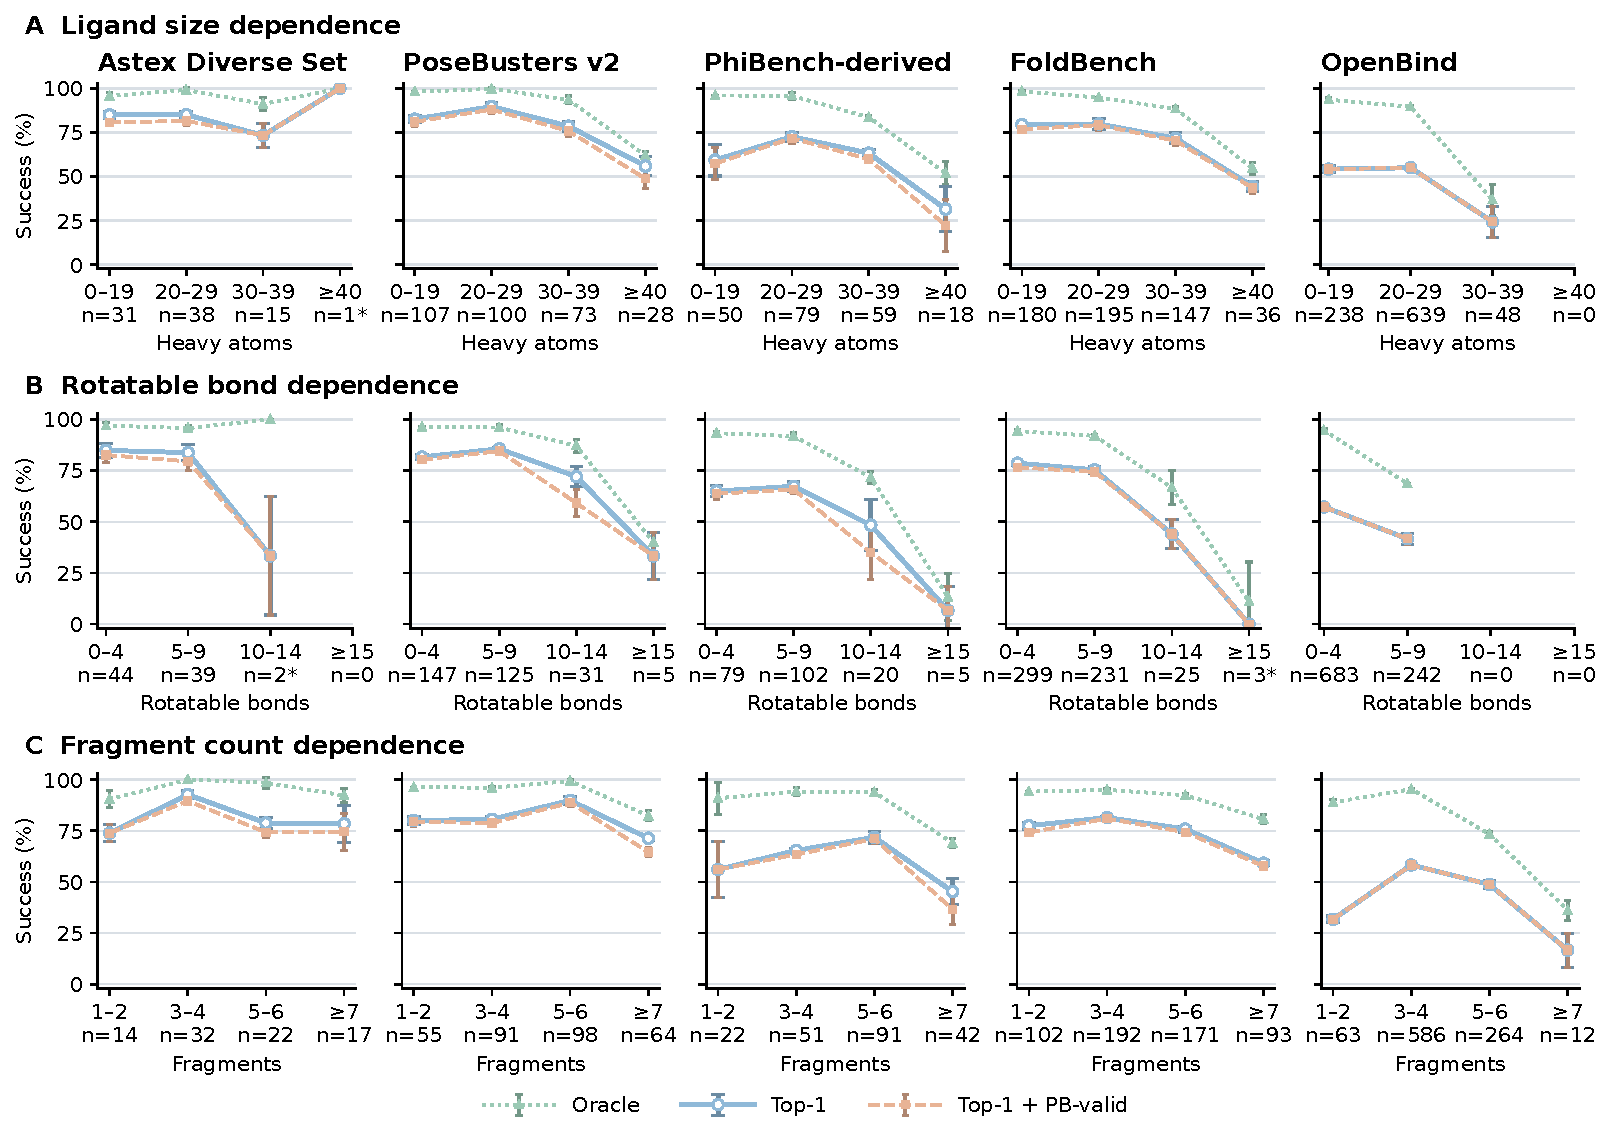
\includegraphics[width=\linewidth,height=0.76\textheight,keepaspectratio]{ligand_complexity.pdf}
    \caption{\textbf{Docking performance across ligand-complexity strata.} \method results use refined candidates and chirality-filtered selection. The five benchmarks are grouped by (A) ligand heavy-atom count, (B) strict rotatable-bond count, and (C) saved rigid-fragment count. Top-1 denotes RMSD \(<2\,\angstrom\); Top-1 + PB-valid requires the same selected pose to pass PoseBusters; Oracle searches all 100 refined candidates using RMSD only. Points show mean \(\pm\) sample SD across three repeats. Labels give unique-complex counts, and asterisks mark bins with fewer than five complexes.}
    \label{fig:si-complexity-performance}
\end{figure}

\begin{figure}[p]
    \centering
    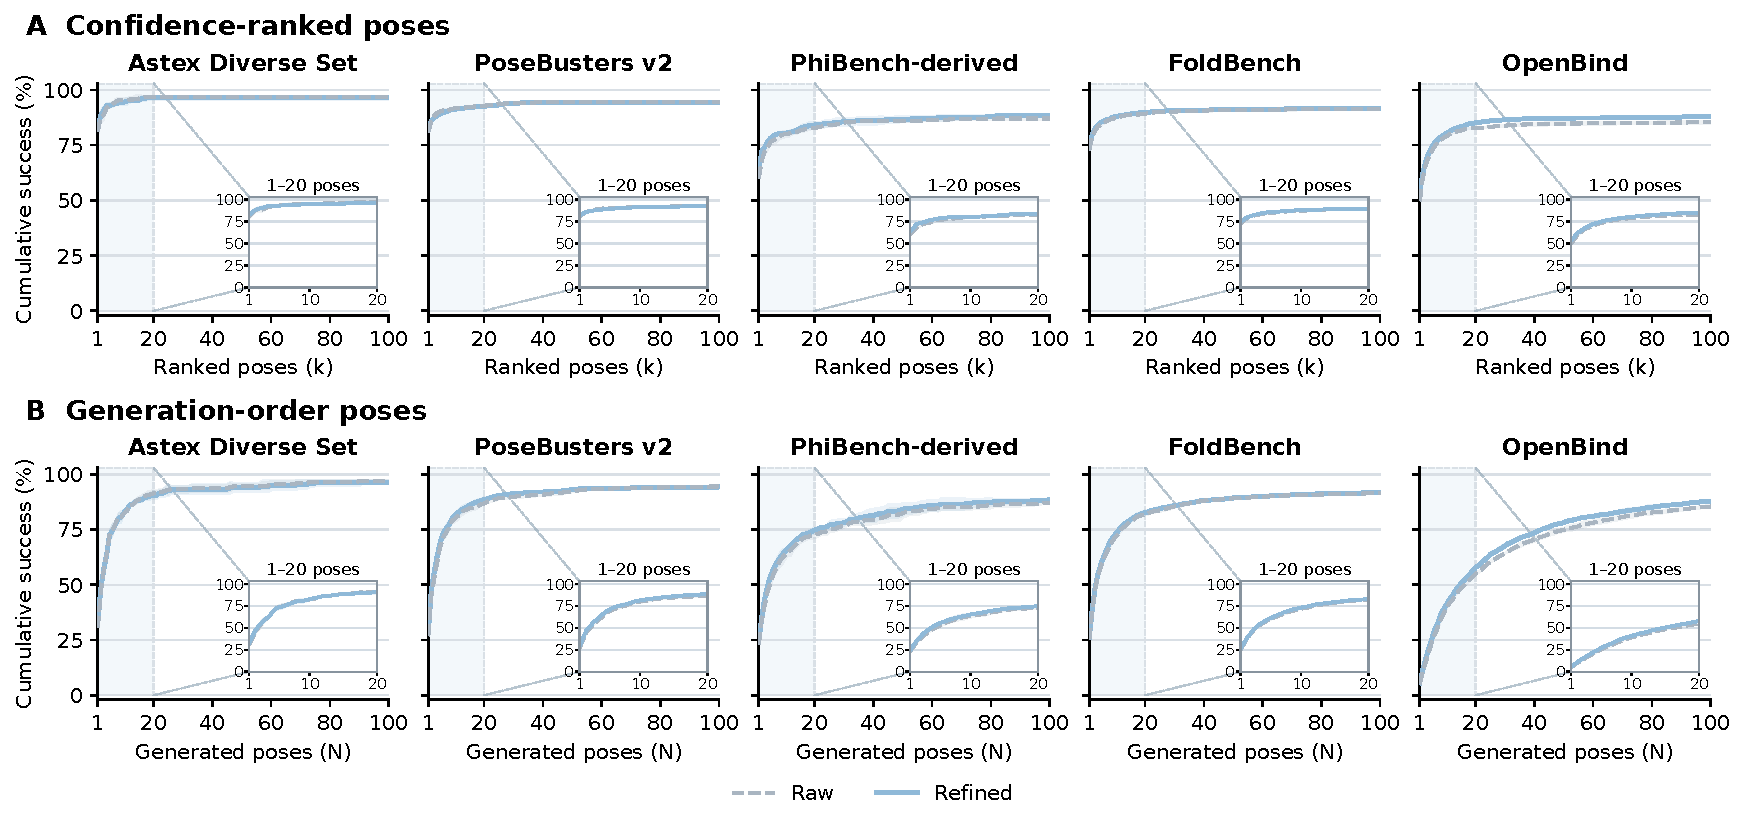
\includegraphics[width=\linewidth,height=0.68\textheight,keepaspectratio]{cumulative_success.pdf}
    \caption{\textbf{Cumulative pose success under confidence ranking and generation order.} \method results are shown for (A) the first \(k\) candidates after unfiltered confidence ranking of the complete bank and (B) the first \(N\) candidates in saved generation order without confidence sorting. Solid and dashed lines denote refined and raw banks; bands show \(\pm1\) sample SD across three repeats. Insets expand candidates 1--20. Both orderings reach the full-bank RMSD-only oracle at 100 poses; PoseBusters validity is not included.}
    \label{fig:si-pose-order}
\end{figure}

\begin{figure}[p]
    \centering
    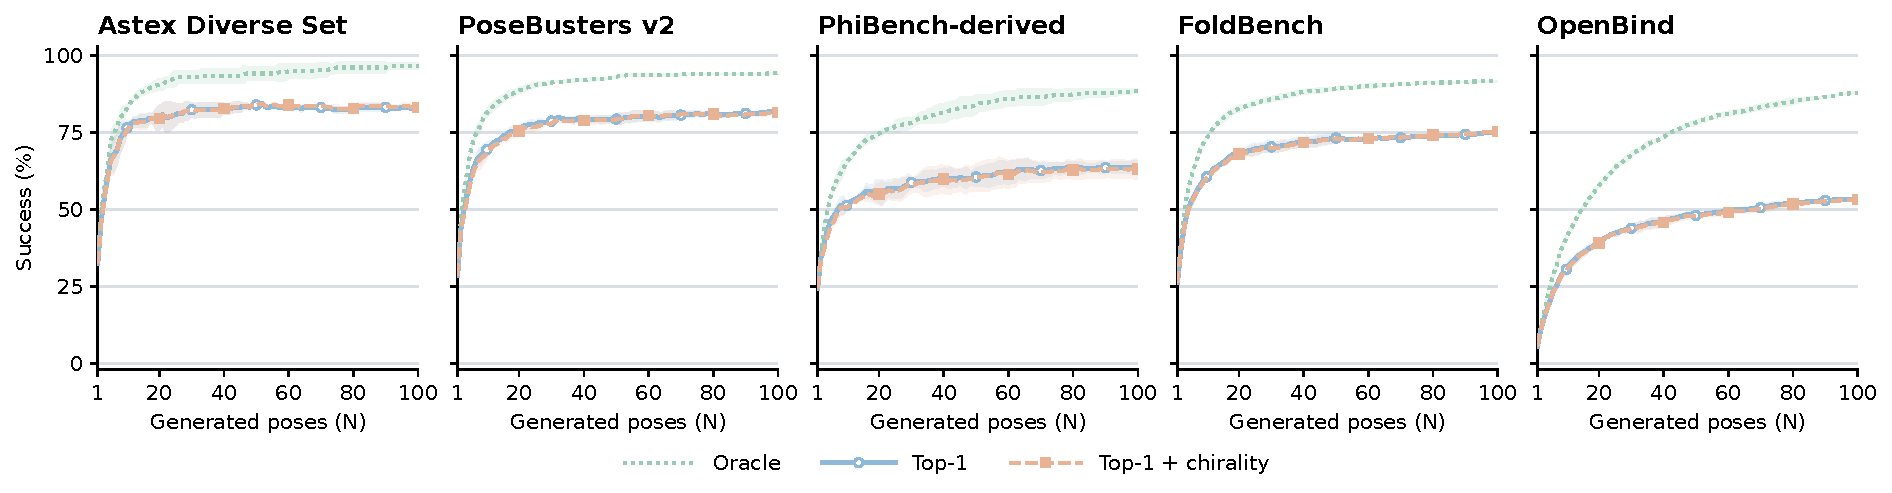
\includegraphics[width=\linewidth,height=0.48\textheight,keepaspectratio]{pose_budget.pdf}
    \caption{\textbf{Selected-pose success as a function of available candidate count.} The first \(N\) refined candidates are retained from each \method 100-pose bank. Top-1 reselects the minimum predicted-RMSD pose, Top-1 + chirality applies the input-chirality mask with the production fallback, and Oracle tests whether the prefix contains any RMSD-successful pose. Lines and bands show mean \(\pm1\) sample SD across three repeats. The curves reuse saved prefixes and are not independently executed smaller campaigns or runtime measurements.}
    \label{fig:si-candidate-prefix}
\end{figure}

\clearpage

\subsection{Resource measurements}

On a single RTX PRO 6000 Blackwell Max-Q GPU, the complete primary protocol for Astex repeat 0 required 8.8\,s per complex for ligand preparation and 100-pose, ten-step generation (single 85-complex process including model loading), a mean of 81.7\,s (median 85.8\,s) for refinement and 9.5\,s (median 9.6\,s) for confidence scoring of the raw and refined banks, or about 100\,s per complex in total. These measurements reran refinement and scoring on the saved raw banks in a separate output location and did not replace any reported outcome; the same candidate was ranked first in 84 of 85 refined banks, the remaining difference reflecting cross-device numerical variation.

The docking model has 5,719,970 parameters; the confidence model has 9,403,274.
Runtime is measured in wall-clock seconds per complex; memory is CUDA allocated memory in GiB (\(2^{30}\) bytes).

Runtime and memory measurements are shown in Figs.~\ref{fig:si-runtime} and \ref{fig:si-generation-memory}. Profiling used mixed RTX A5000, RTX 6000 Ada and RTX PRO 6000 devices. Recorded times include the original refinement and confidence scoring but exclude subsequent refinement and rescoring passes; the single-device stage costs above, rather than these profiles, describe the primary protocol, and the profiles do not support a controlled hardware comparison.

\begin{figure}[!htbp]
    \centering
    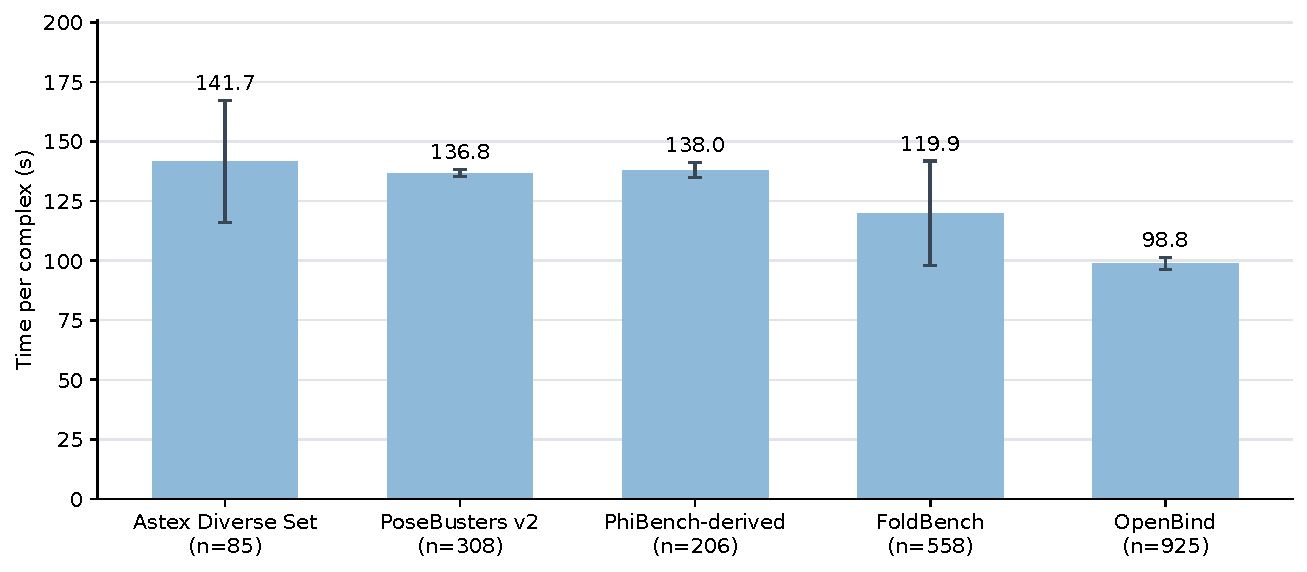
\includegraphics[width=\linewidth,height=0.42\textheight,keepaspectratio]{historical_runtime.pdf}
    \caption{\textbf{Initial candidate-acquisition pipeline runtime.} Mean wall time per complex for the unguided 100-pose, 10-step evaluation. Runtime covers setup, generation, original refinement and confidence scoring, and I/O. It excludes official PoseBusters evaluation and subsequent refinement and rescoring passes, so it is not the end-to-end runtime of the primary results. Whiskers show sample SD across three fixed-weight inference repeats. Mixed devices and cohort-specific process profiles preclude a controlled speed comparison.}
    \label{fig:si-runtime}
\end{figure}

\begin{figure}[p]
    \centering
    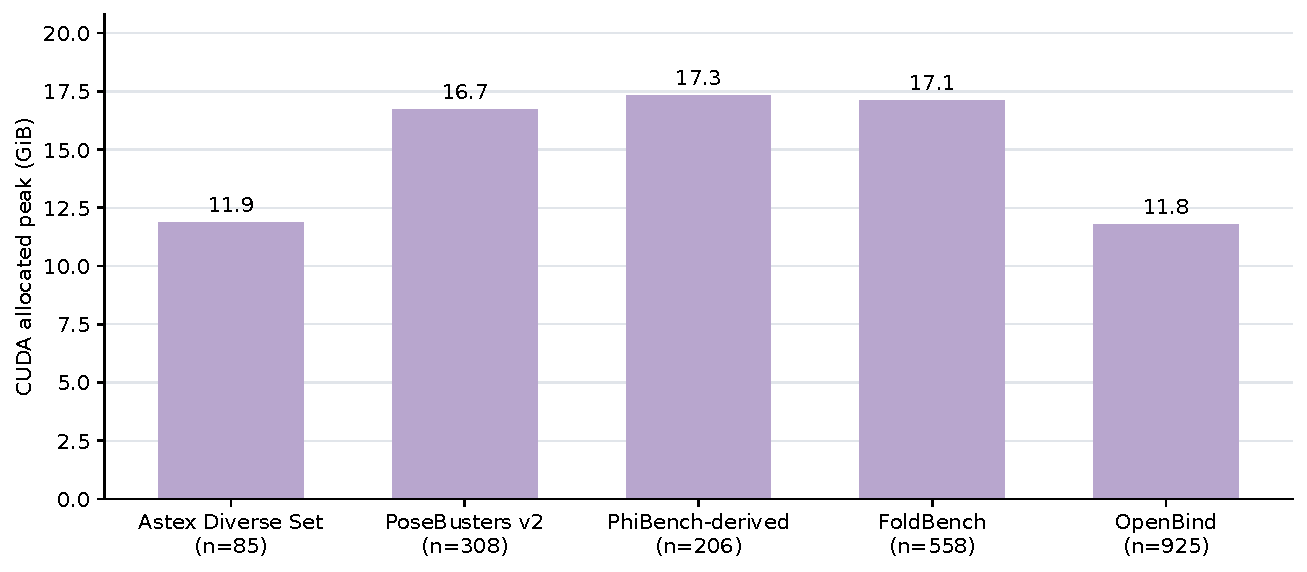
\includegraphics[width=\linewidth,height=0.42\textheight,keepaspectratio]{generation_memory.pdf}
    \caption{\textbf{Initial pose-generation process memory.} Maximum CUDA allocated-memory peak across three repeats of the unguided 100-pose, 10-step evaluation. This is the original generation/evaluation process allocator peak, not reserved memory or a whole-pipeline peak. Astex Diverse Set and PoseBusters v2 used candidate-only generation processes, whereas PhiBench-derived, FoldBench and OpenBind processes included initial confidence scoring. Separate post-generation refinement and rescoring processes are excluded. Mixed devices and these different process profiles preclude a controlled comparison of sampling-only memory.}
    \label{fig:si-generation-memory}
\end{figure}

\clearpage

\subsection{Training-set relatedness}

Training-set relatedness varied across cohorts (Figs.~\ref{fig:si-relatedness-overview}--\ref{fig:si-relatedness-sequence}). All OpenBind complexes occupied the highest sequence-identity bin. FoldBench had the greatest same-training-sample overlap: 63.4\% shared an exact ligand match and at least 70\% sequence identity, whereas this conjunction was absent in docking validation. PDB-accession sharing is distinct from joint ligand--sequence overlap because an accession can contain different chains or ligands; accession correspondence was unavailable for OpenBind. Neither ligand nor sequence relatedness showed a consistent monotonic association with success.
In the overlap legend, same-sample means an observed exact ligand match and binding-chain identity of at least 70\% in the same training sample; separate matches satisfy the two criteria in different samples without such a joint match. Ligand-only and sequence-only satisfy one criterion, and neither observed indicates absence of both observed matches. The 70\% identity threshold is a descriptive overlap rule, distinct from PLINDER pocket-community membership. In the ligand-similarity bins, \(T\) denotes Tanimoto similarity, not the selected-success rate \(T\) used in failure decomposition.

\begin{figure}[!htbp]
    \centering
    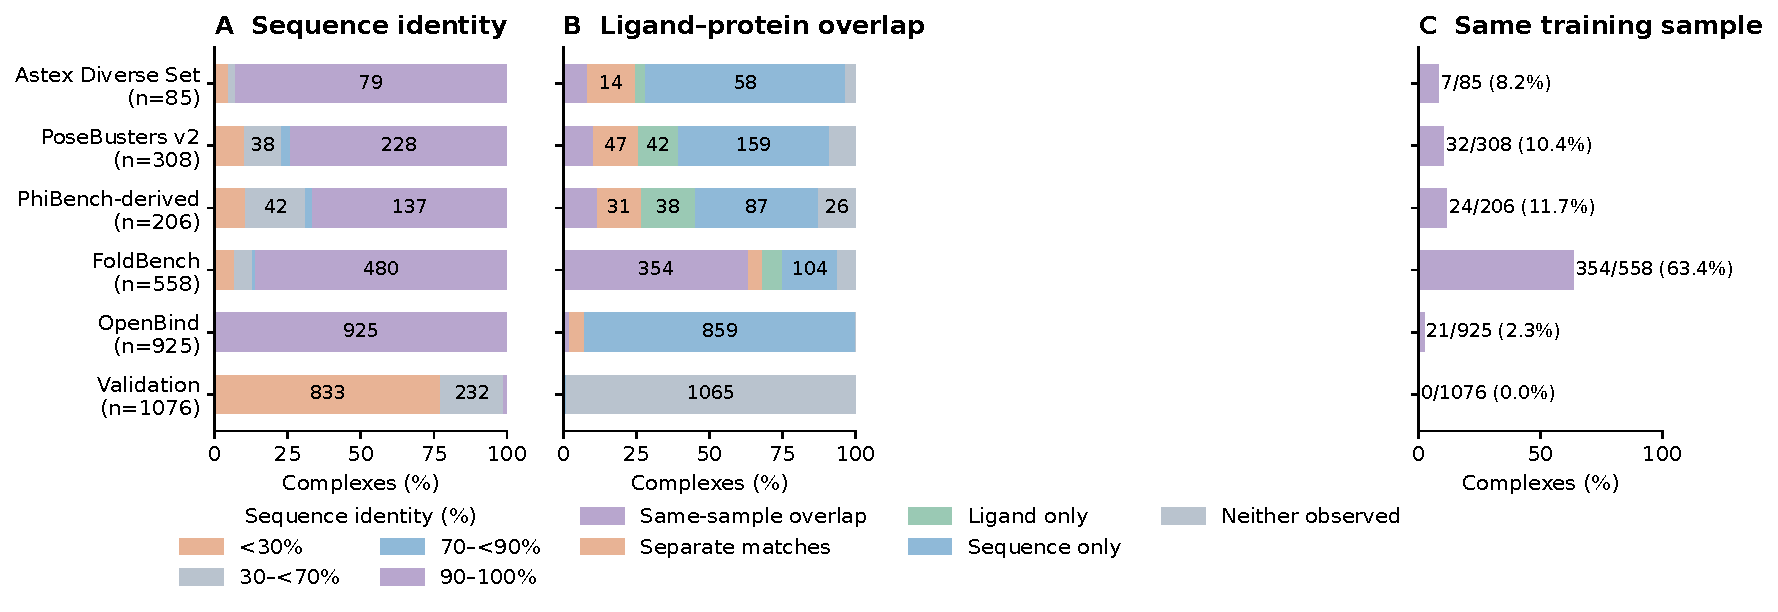
\includegraphics[width=\linewidth,height=0.62\textheight,keepaspectratio]{training_relatedness.pdf}
    \caption{\textbf{Sequence and ligand relatedness to the docking-training set.} The five external cohorts and 1,076-complex docking-validation set are compared with 47,277 executed docking-training samples. (A) Maximum query-normalized binding-chain sequence identity. (B) Joint ligand and sequence overlap classified by whether the matches occur in the same training sample. (C) The same-sample overlap fraction with counts. Ligand-binding chains use protein--ligand heavy-atom contacts within \(6\,\angstrom\).}
    \label{fig:si-relatedness-overview}
\end{figure}

\begin{figure}[p]
    \centering
    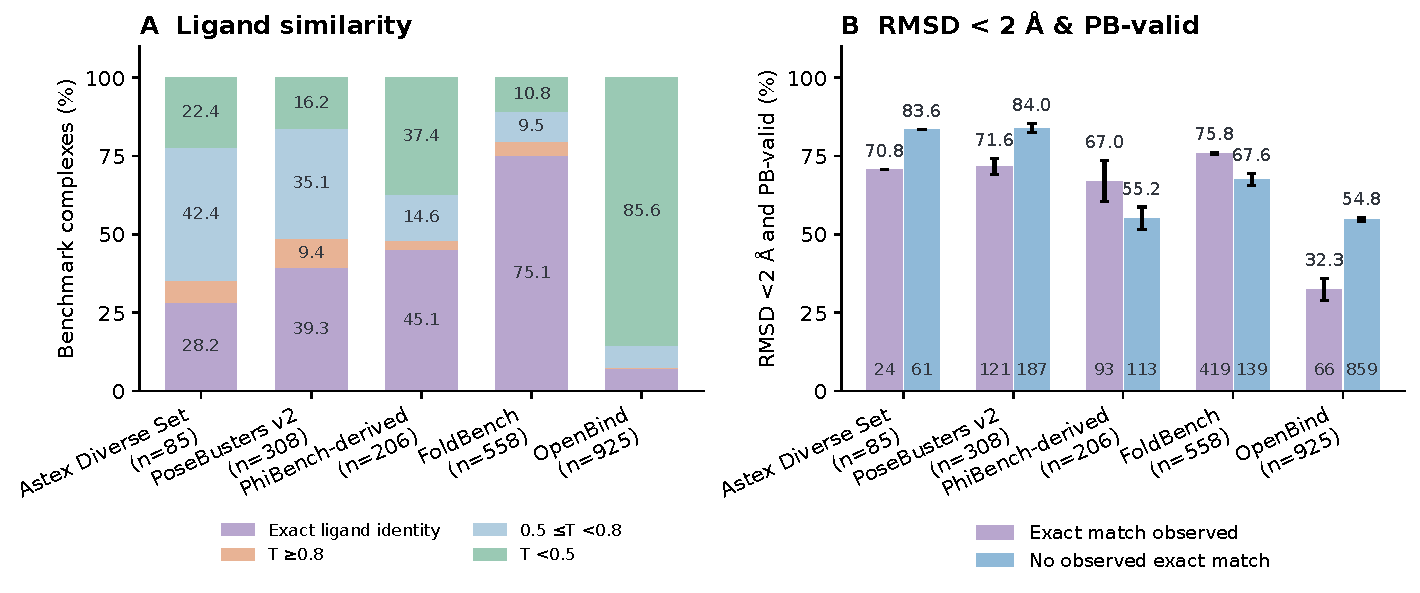
\includegraphics[width=\linewidth,height=0.58\textheight,keepaspectratio]{ligand_similarity.pdf}
    \caption{\textbf{Training-ligand relatedness and stratified docking performance.} (A) Exact heavy-isomeric ligand identity and nearest training-ligand Morgan-fingerprint Tanimoto similarity relative to the 47,277 executed docking-training samples. T denotes nearest-neighbour Tanimoto similarity. (B) \method RMSD--PoseBusters success with and without an observed exact ligand match; numbers at the base of the bars are group sizes. Bars show mean \(\pm\) sample SD across three repeats; group differences are descriptive and confounded by cohort composition.}
    \label{fig:si-relatedness-ligand}
\end{figure}

\begin{figure}[p]
    \centering
    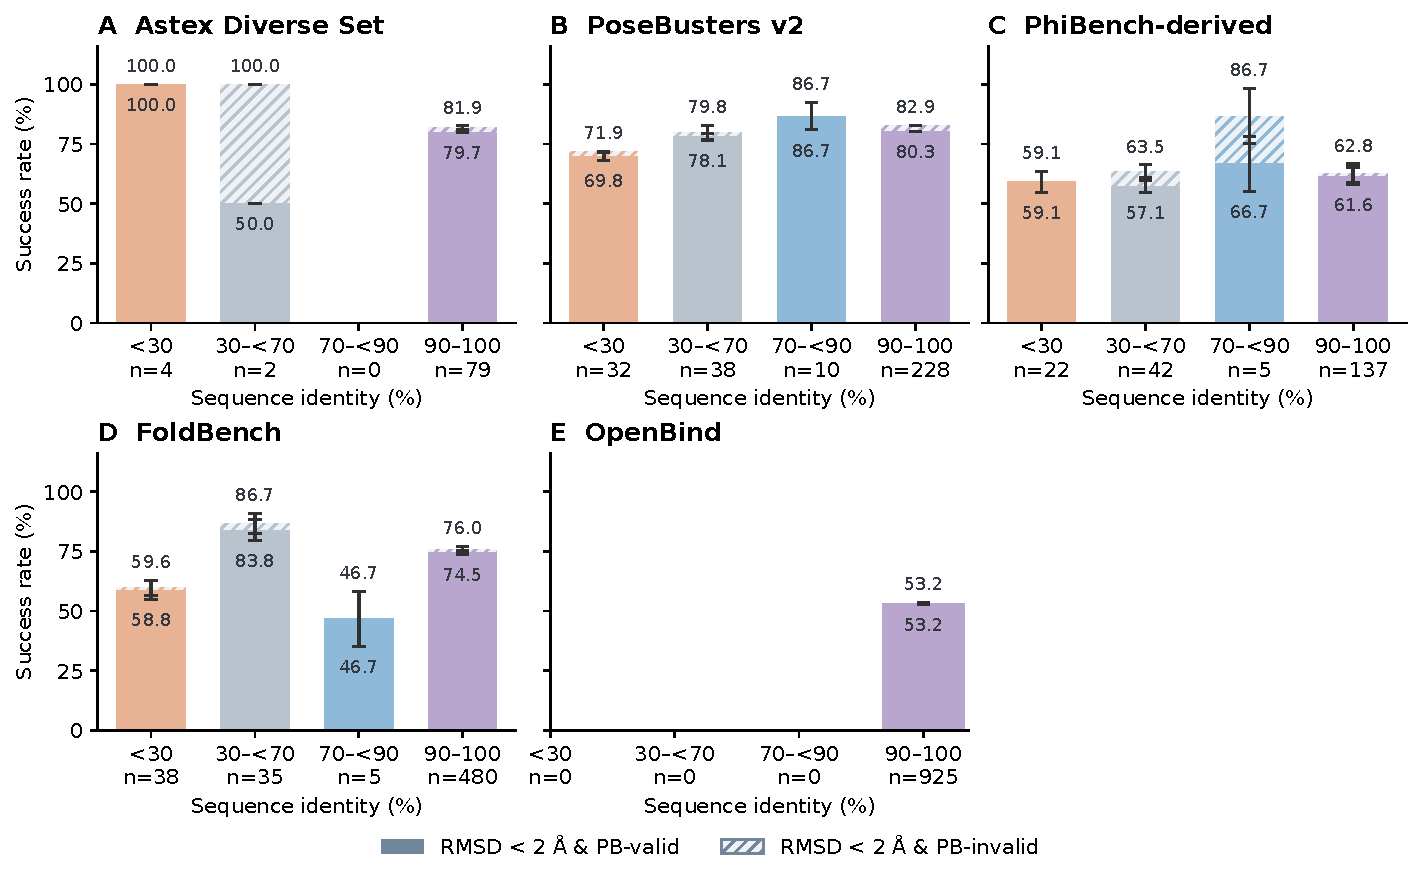
\includegraphics[width=\linewidth,height=0.68\textheight,keepaspectratio]{sequence_similarity.pdf}
    \caption{\textbf{Docking performance by training-set sequence identity.} Strata use maximum query-normalized binding-chain identity to the docking-training set. Solid bars show RMSD--PoseBusters success, coloured by identity stratum (the dark legend patch denotes solid fill); hatching extends to RMSD-only success. Bars and whiskers show three-repeat means and sample SD; labels give stratum sizes, including empty and sparse groups.}
    \label{fig:si-relatedness-sequence}
\end{figure}

\clearpage

\subsection{Paired improvements and failure decomposition}

Figs.~\ref{fig:si-paired-effects}--\ref{fig:si-complexity-failures} separate the paired effect of post-processing, the density of useful candidates, and the stage at which each complex fails.

\begin{figure}[p]
    \centering
    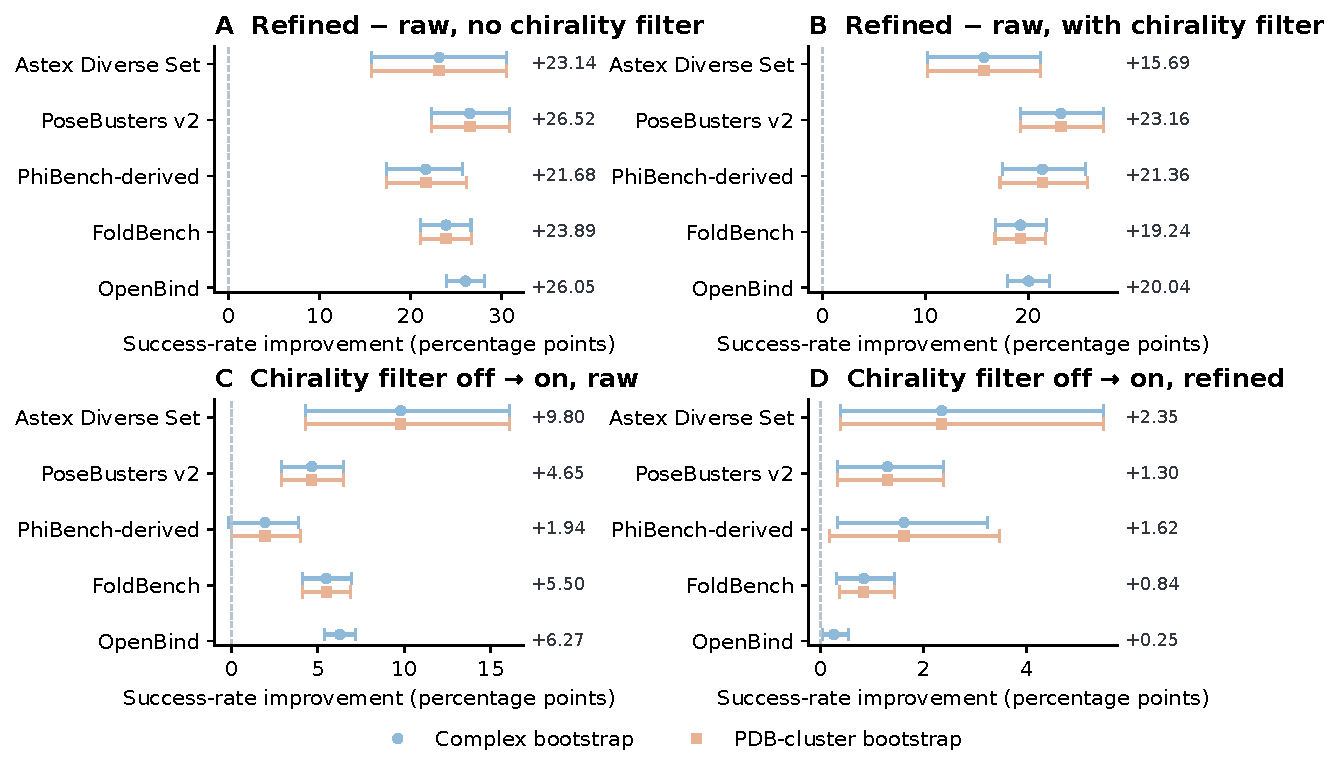
\includegraphics[width=\linewidth,height=0.68\textheight,keepaspectratio]{paired_uncertainty.pdf}
    \caption{\textbf{Paired changes in docking success with refinement and chirality filtering.} \method results compare refined versus raw candidates with and without the chirality filter and filter off versus on at each stage. The endpoint is RMSD \(<2\,\angstrom\) and PoseBusters success. Per-complex paired differences are averaged across seeds before 2,000-draw percentile bootstrapping. Whiskers show complex and exact-PDB-cluster 95\% intervals; OpenBind lacks a cluster interval.}
    \label{fig:si-paired-effects}
\end{figure}

\begin{figure}[p]
    \centering
    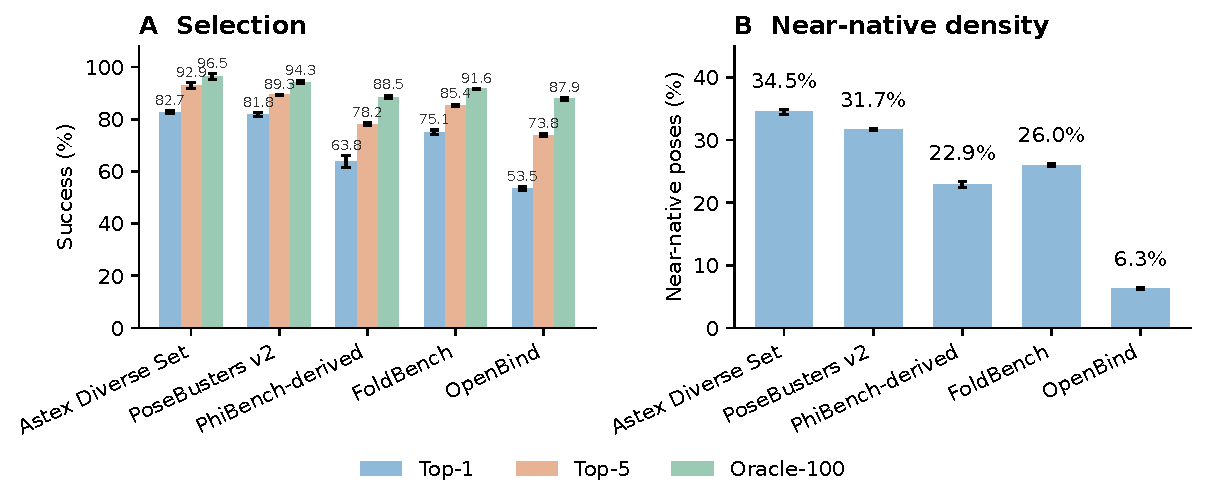
\includegraphics[width=\linewidth,height=0.56\textheight,keepaspectratio]{candidate_ranking.pdf}
    \caption{\textbf{Confidence selection and near-native candidate density.} (A) Unfiltered confidence top-1, top-5, and oracle-100 RMSD success for refined unguided banks; the primary chirality-filtered top-1 values are given in Fig.~\ref{fig:si-stringent-slices}. (B) Fraction of individual refined candidates with RMSD \(<2\,\angstrom\). Bars show mean \(\pm\) sample SD across three repeats. Panel A is measured per complex, whereas panel B is measured per candidate.}
    \label{fig:si-selection-density}
\end{figure}

\begin{figure}[p]
    \centering
    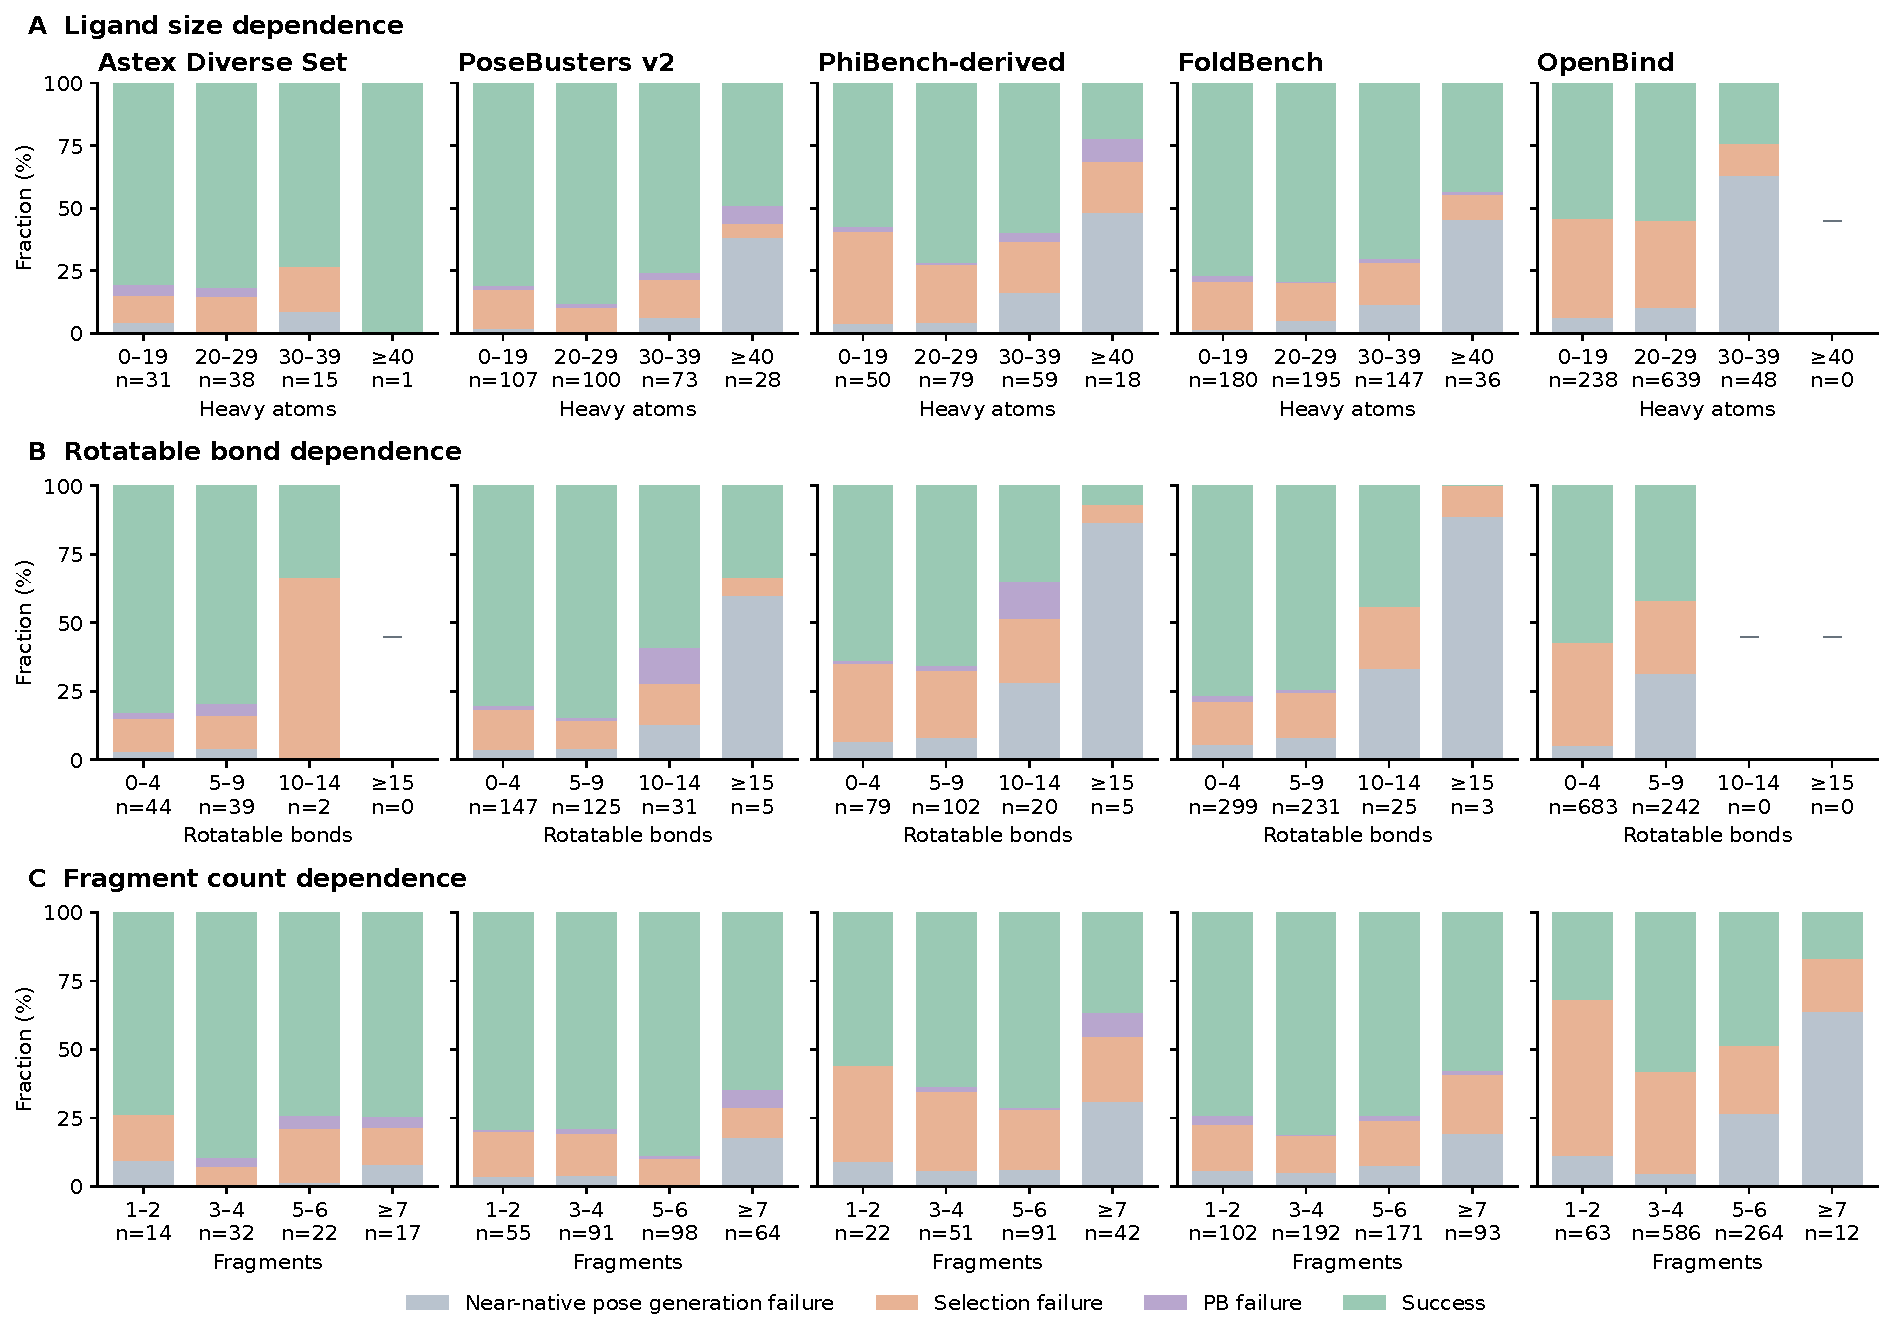
\includegraphics[width=\linewidth,height=0.76\textheight,keepaspectratio]{complexity_failures.pdf}
    \caption{\textbf{Descriptive failure decomposition across ligand-complexity strata.} \method, refined, chirality-filtered outcomes are partitioned into no RMSD-successful candidate, an available successful candidate not selected, selected RMSD success with PoseBusters failure, or RMSD--PoseBusters success. The fractions are the algebraic decomposition \(100-O\), \(O-T\), \(T-J\), and \(J\) of oracle coverage \(O\), selected RMSD success \(T\), and RMSD--PoseBusters success \(J\). The \(100-O\) category denotes absence of an RMSD-successful candidate after refinement. The \(O-T\) category combines chirality exclusion and ranking loss, which main Fig.~5C separates. The legend label ``near-native pose generation failure'' denotes this \(100-O\) category; dashes mark empty strata, and strata with fewer than five complexes are too sparse for interpretation.}
    \label{fig:si-complexity-failures}
\end{figure}

\clearpage

\subsection{Confidence reliability and restricted evaluations}

Fig.~\ref{fig:si-confidence-reliability} complements the within-bank rank diagnostics in the main text with empirical reliability curves.
The stringent slices in Fig.~\ref{fig:si-stringent-slices} are small, predefined evaluation subsets defined by the simultaneous ligand and sequence criteria and are therefore descriptive rather than population-level estimates.
Probability bins have boundaries 0.1, 0.2, \(\ldots\), 0.9; predicted-RMSD bins have boundaries 1, 2, 3, 4, 6 and 10 Å. Bin summaries pool candidates across repeats, with boundary values assigned to the higher bin. Near-native-count groups are 0, 1--5, 6--20, 21--50 and 51--100. Bins are fixed display strata. Identity \(<30\%\) and Tanimoto \(<0.5\), together with no observed exact ligand match, define the low-relatedness slice.

\begin{figure}[p]
    \centering
    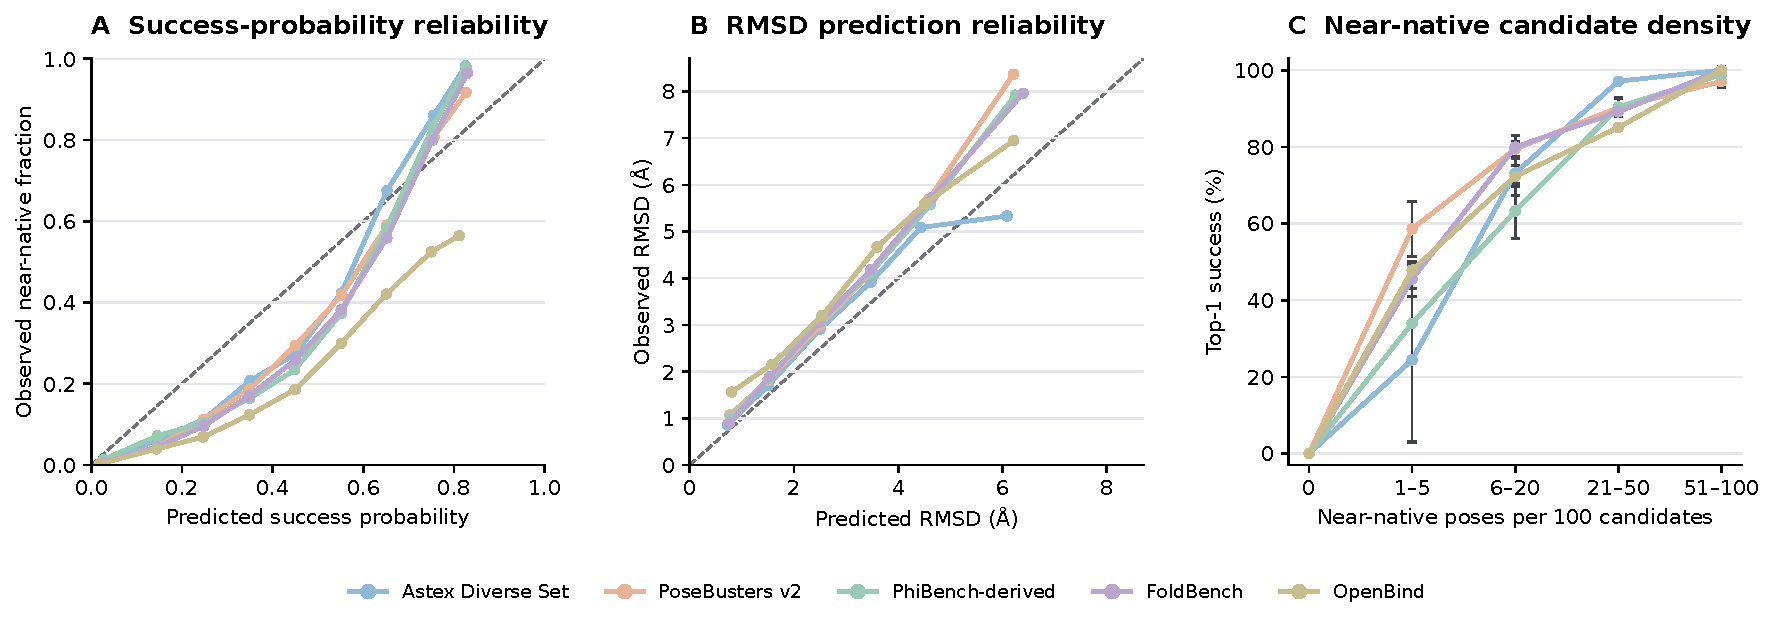
\includegraphics[width=\linewidth,height=0.62\textheight,keepaspectratio]{confidence_reliability.pdf}
    \caption{\textbf{Reliability of saved confidence predictions and candidate-density dependence.} \method refined candidates are pooled across three repeats. (A) Empirical near-native fraction versus the saved success-head probability. (B) Mean observed versus predicted RMSD in fixed predicted-RMSD bins. No recalibration is fitted. (C) Primary chirality-filtered top-1 RMSD success versus the number of near-native candidates in the 100-pose bank; whiskers show sample SD across three repeats. Candidate observations within complexes are correlated, and the production selector uses predicted RMSD rather than the auxiliary probability head.}
    \label{fig:si-confidence-reliability}
\end{figure}

\begin{figure}[p]
    \centering
    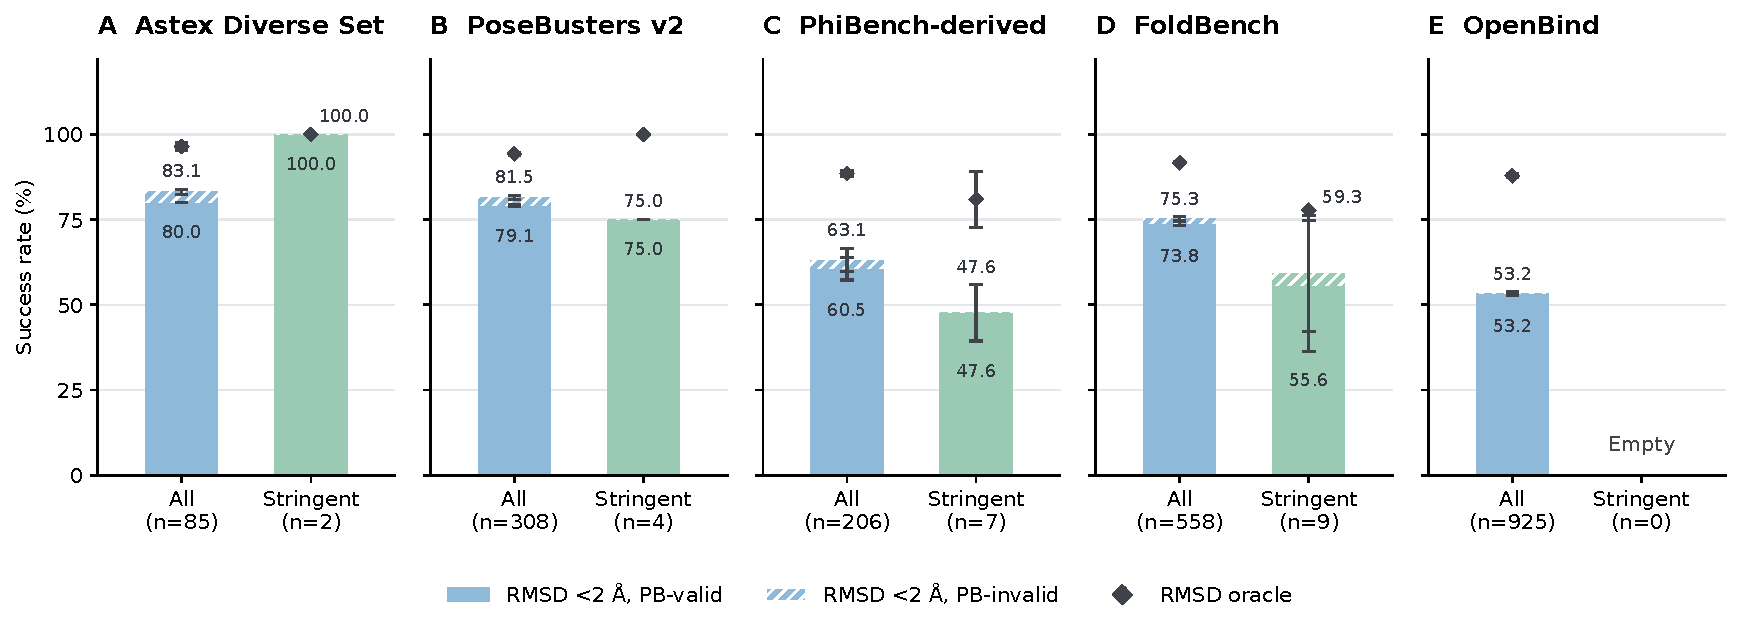
\includegraphics[width=\linewidth,height=0.58\textheight,keepaspectratio]{stringent_subset.pdf}
    \caption{\textbf{Performance under simultaneous sequence and ligand restrictions.} The fixed subset requires maximum training-relative binding-chain identity \(<30\%\), Morgan Tanimoto \(<0.5\), and no observed exact training-ligand match. Selected RMSD and RMSD--PoseBusters success and full-bank RMSD oracle are shown for EFF-Dock. Blue bars show all complexes and green bars the stringent subset. Remaining counts are 2, 4, 7, 9 and 0 for Astex Diverse Set, PoseBusters v2, PhiBench-derived, FoldBench and OpenBind, respectively; the slices are descriptive.}
    \label{fig:si-stringent-slices}
\end{figure}

\clearpage

\subsection{Paired baseline uncertainty and trajectory visualization}

Fig.~\ref{fig:si-baseline-differences} reports paired uncertainty for the locally executed baseline comparisons, and Fig.~\ref{fig:si-generation-trajectory} shows the saved one-pose trajectory used for the workflow illustration.

\begin{figure}[p]
    \centering
    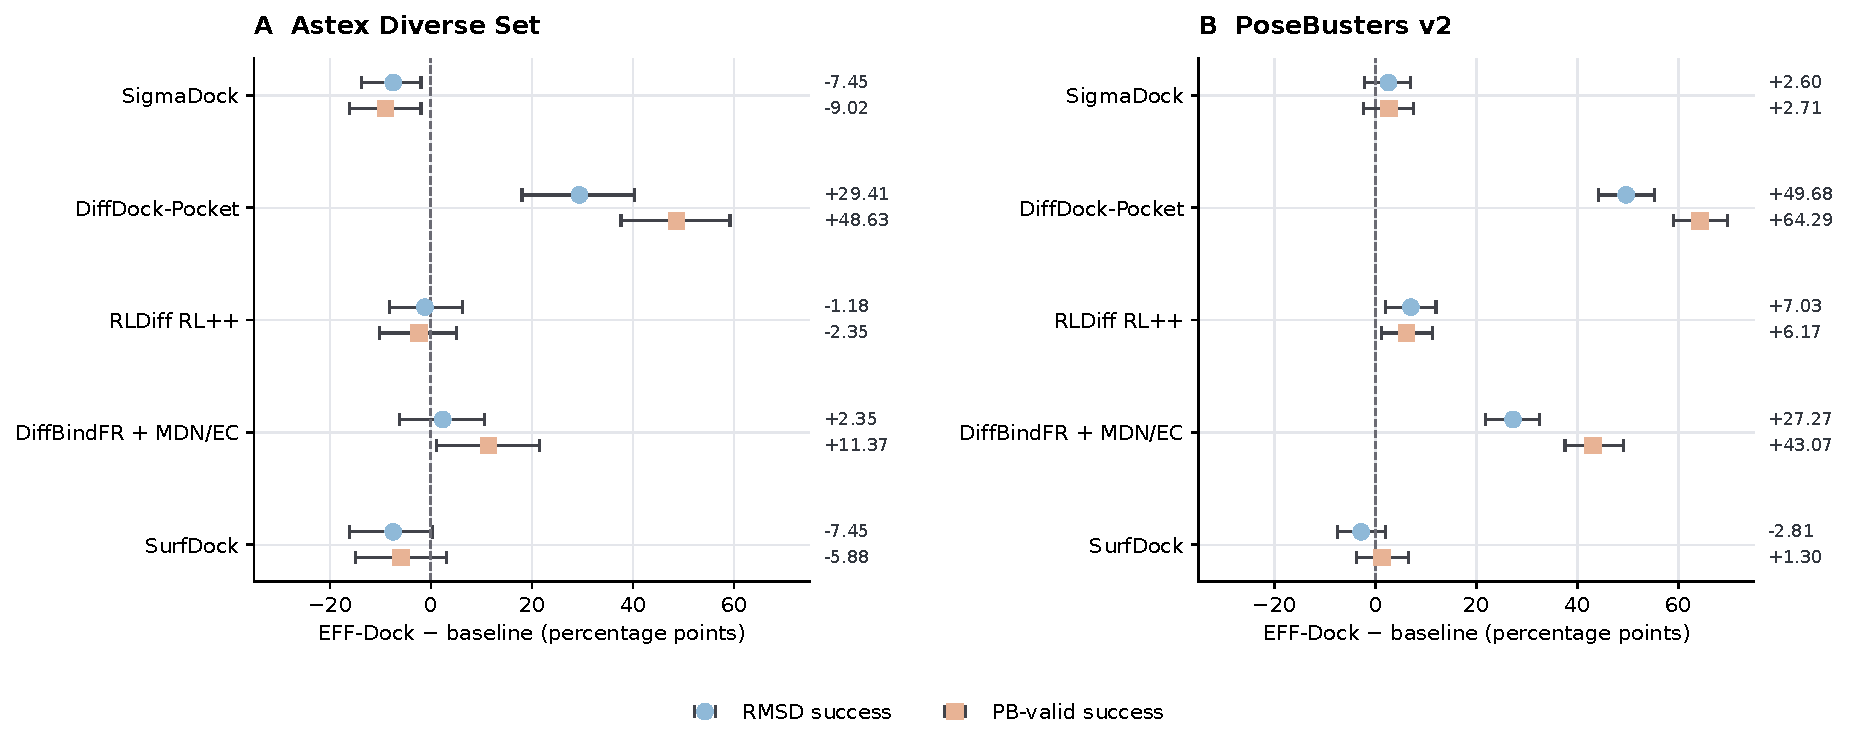
\includegraphics[width=\linewidth,height=0.62\textheight,keepaspectratio]{baseline_uncertainty.pdf}
    \caption{\textbf{Paired uncertainty relative to locally executed baselines.} \method minus baseline percentage-point differences are shown for RMSD success and same-selected-pose RMSD--PoseBusters success (legend: PB-valid success) on (A) Astex Diverse Set and (B) PoseBusters v2. Intervals are 2,000-draw percentile 95\% paired bootstrap intervals over exact PDB-accession groups; every retained complex has a distinct accession in these cohorts. Literature-only rows are excluded. Positive values favor EFF-Dock, but differing budgets and native selectors prevent an equal-compute superiority claim.}
    \label{fig:si-baseline-differences}
\end{figure}

\begin{figure}[p]
    \centering
    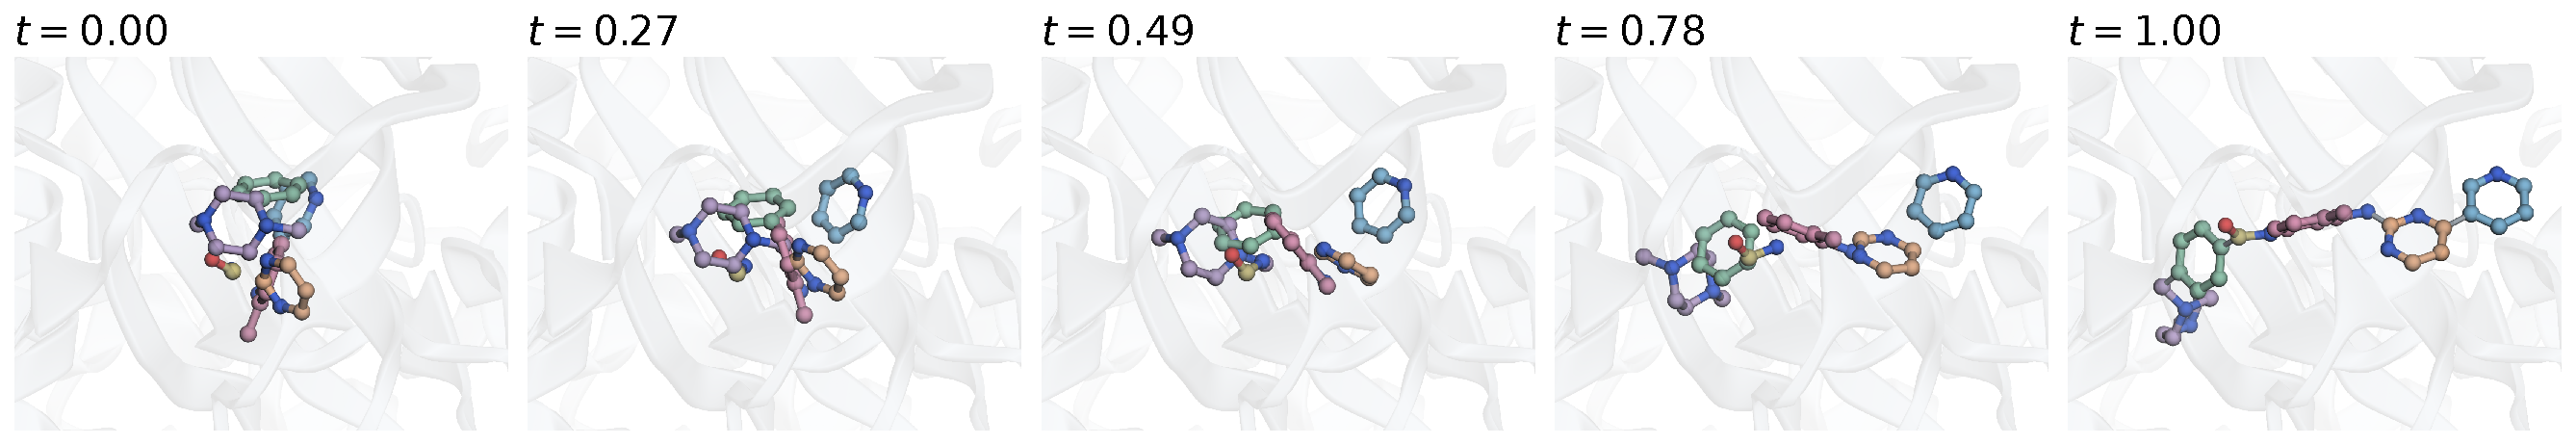
\includegraphics[width=\linewidth,height=0.34\textheight,keepaspectratio]{fragment_trajectory.pdf}
    \caption{\textbf{Fragment motion along a saved ODE trajectory.} Astex 1T46--STI at five saved flow times in a fixed receptor frame. Colors track six rigid fragments; omission of early interfragment bonds is a display convention. Dimensionless flow time describes generation, separate from refinement. This prespecified seed-42, unguided one-pose illustration starts from the supplied conformer and is separate from the 100-pose benchmark banks, which use conformers generated from SMILES.}
    \label{fig:si-generation-trajectory}
\end{figure}

\clearpage

\subsection{Physical validity and representative structures}

Physical-validity failures are reported in Fig.~\ref{fig:pb-failure-profiles}. Raw and refined selection may identify different candidates; matched-index transitions in this figure are limited to the selection-biased subset evaluated at both stages. For Astex and PoseBusters v2, Section~\ref{si:all_candidate_pb} follows every candidate through refinement.

\begin{figure}[!htbp]
    \centering
    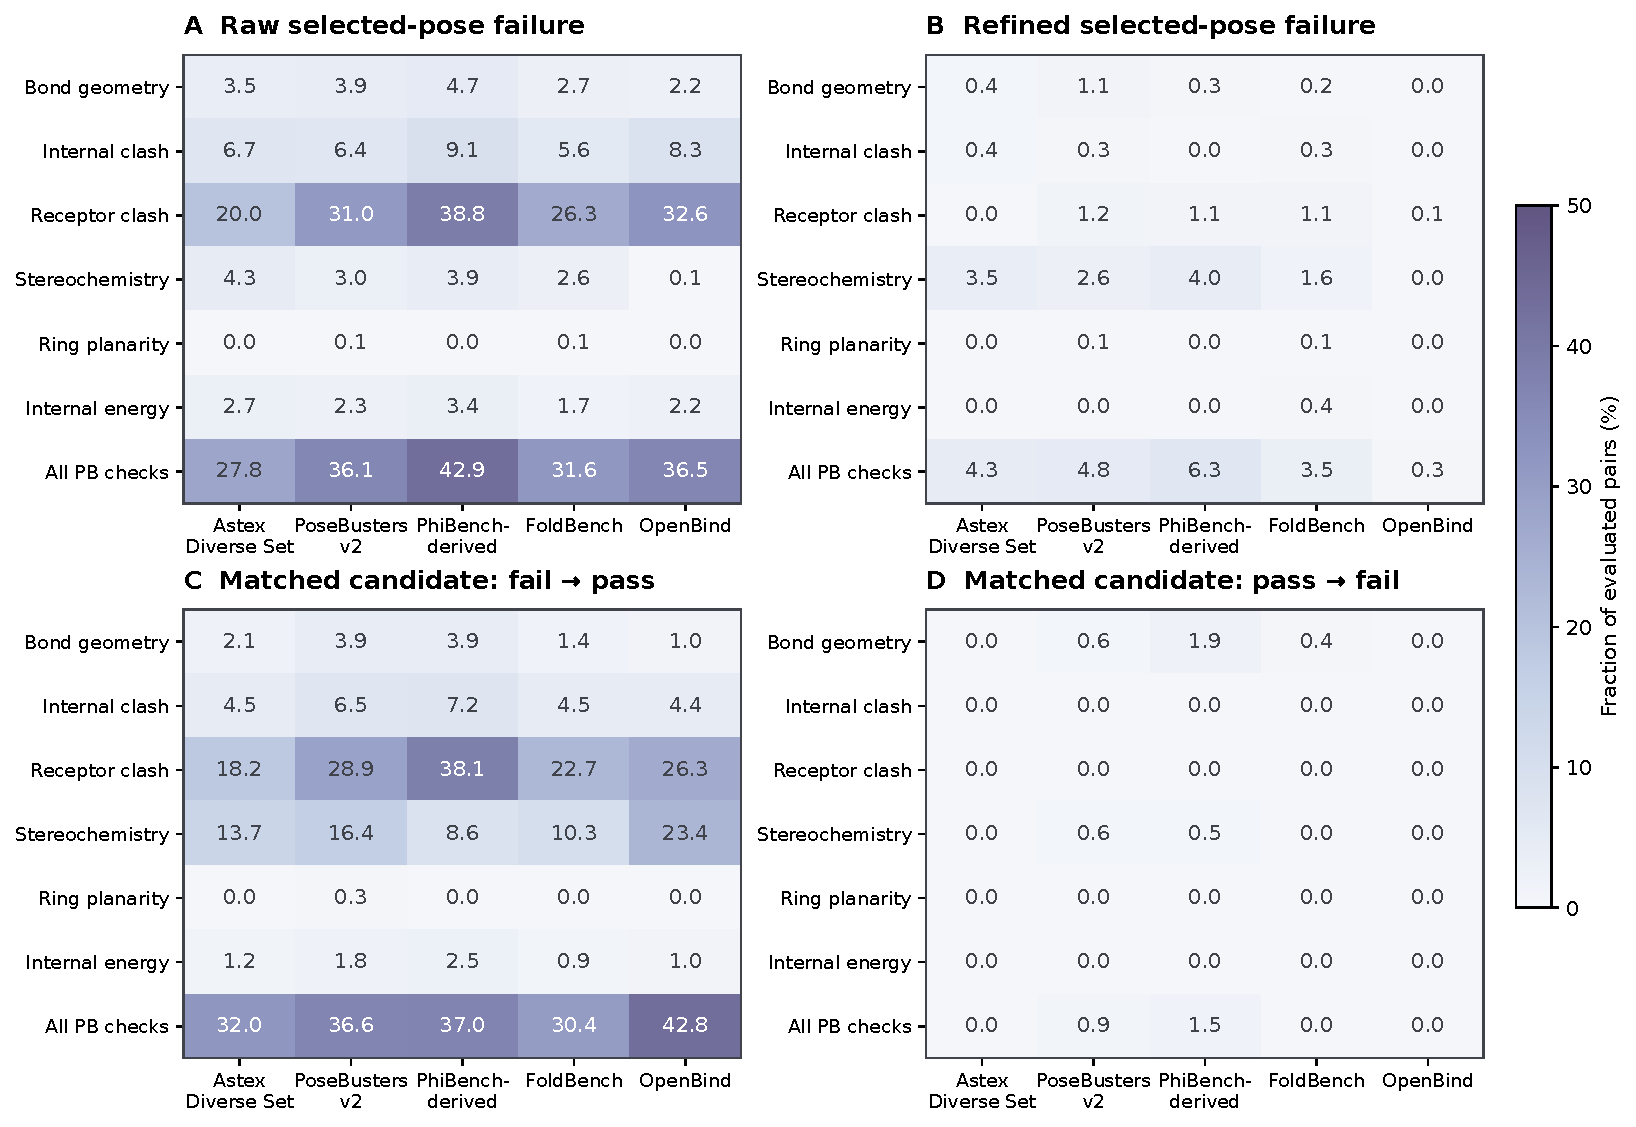
\includegraphics[width=\linewidth,height=0.76\textheight,keepaspectratio]{physical_validity.pdf}
    \caption{\textbf{Physical-validity failures before and after refinement.} (A,B) Heatmaps report failure percentages among the primary selected raw and refined poses; the selected candidate may differ between stages. (C,D) Fail-to-pass and pass-to-fail percentages use candidate indices with saved official PoseBusters evaluations at both stages. Rows summarize bond geometry, internal clash, receptor clash, stereochemistry, ring planarity, internal energy, and all 27 non-RMSD checks. Categories overlap, and the matched subset is selection biased; its fail-to-pass rates therefore differ from the all-candidate transitions in Sec.~\ref{si:all_candidate_pb}. The colour scale gives percentages for all four panels.}
    \label{fig:pb-failure-profiles}
\end{figure}

Fig.~\ref{fig:representative-cases} illustrates selected-pose success, refinement rescue and selection failure in each cohort. These cases are selected by a deterministic rule rather than random sampling. Each rescue shows the largest same-candidate RMSD decrease satisfying raw RMSD \(\ge2\,\angstrom\), refined RMSD \(<2\,\angstrom\), and selected-pose PoseBusters validity; it should not be interpreted as a typical effect.

\begin{figure}[!htbp]
    \centering
    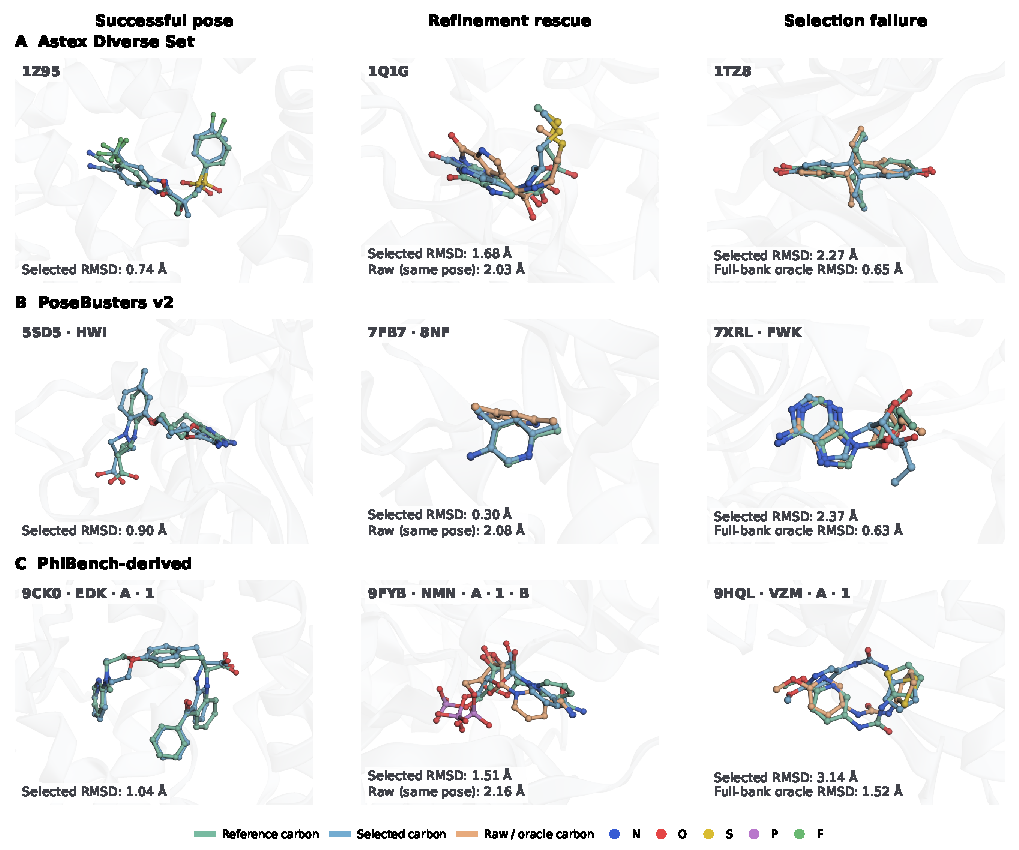
\includegraphics[width=\linewidth,height=0.78\textheight,keepaspectratio]{structure_examples.pdf}
    \caption{\textbf{Dataset-specific examples of success, refinement rescue, and selection failure.} (A--C) Astex Diverse Set, PoseBusters v2 and PhiBench-derived; (D,E) FoldBench and OpenBind appear on the continuation page. Rescue panels show the largest same-candidate RMSD decrease meeting the stated success and validity criteria in each dataset. Successful and selection-failure cases are deterministic lower-median examples from the remaining qualifying records. Rescue panels therefore show extremes rather than typical effects. Coordinates remain in the receptor frame without independent ligand alignment. A failed primary selection is compared with the minimum-RMSD pose from the full saved bank; this comparator is not required to pass the chirality screen or PoseBusters and does not by itself isolate a confidence-ranking failure.}
    \label{fig:representative-cases}
\end{figure}

\clearpage
\begin{figure}[!htbp]
    \centering
    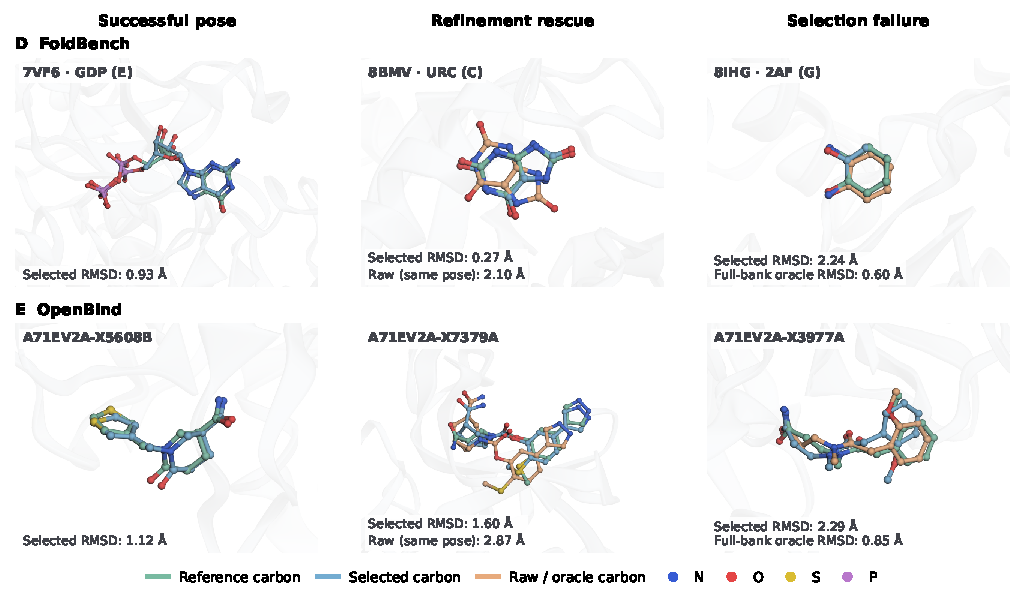
\includegraphics[width=\linewidth,height=0.78\textheight,keepaspectratio]{structure_examples_continued.pdf}
    \par\smallskip
    {\small\textbf{Supplementary Fig.~\ref{fig:representative-cases} (continued).} (D,E) FoldBench and OpenBind examples, with the same structure, color and candidate-selection conventions as panels A--C.}
\end{figure}
\clearpage

\subsection{Eligibility-aware failure decomposition}

Main Fig.~5C partitions outcomes using the same effective eligible set as the primary selector, including its unfiltered fallback; Fig.~\ref{fig:selection-bottlenecks} reports the corresponding regret. For all five cohorts this partition defines candidate-bank success by RMSD alone. For Astex and PoseBusters v2, Section~\ref{si:all_candidate_pb} adds official PoseBusters labels for every candidate and repeats the partition with joint RMSD--PoseBusters success.

\subsection{All-candidate PoseBusters evaluation}
\label{si:all_candidate_pb}

Every raw and refined candidate in the primary Astex and PoseBusters v2 banks was evaluated with PoseBusters 0.6.5 in \texttt{redock} mode against the same reference ligand and receptor used for the selected-pose endpoint (85 and 308 complexes, three repeats, 100 candidates per bank and stage; 235,800 poses). Before any summary, the recomputed checks for each selected and default-ranked candidate were required to equal the saved selected-pose checks; all banks passed this test. A candidate is jointly successful when its symmetry-aware RMSD is below \(2\,\angstrom\) and it passes all 27 non-RMSD checks. The joint oracle records whether any jointly successful candidate exists in a bank, and the eligible joint oracle restricts this to the effective chirality-eligible set. PoseBusters labels do not enter the primary selector; they are used only for retrospective analyses, including the explicitly labelled PB-filtered selector.

The joint partition assigns each complex to exactly one state: no RMSD-successful candidate; RMSD-successful candidates but none passing PoseBusters; jointly successful candidates but none eligible; an eligible jointly successful candidate that was not selected (joint ranking failure); or a selected jointly successful pose. Rates use all complexes as the denominator; conditional selection rates use complexes with an eligible jointly successful candidate. Complex-level bootstrap intervals (10,000 resamples, repeats kept paired) describe uncertainty over complexes, not over training runs. Same-index raw-to-refined transitions compare each candidate with its own refined coordinates.

Table~\ref{tab:si_allcand_validity} summarizes candidate-level validity and oracles, and Table~\ref{tab:si_allcand_partition} gives the joint partition. Refinement raised the fraction of candidates passing all checks from about one quarter to 88\%, and the validity of RMSD-successful candidates from 37--43\% to 94\%. Following each candidate through refinement, 61.2\% (Astex) and 64.3\% (PoseBusters v2) of candidates changed from failing to passing PoseBusters and 0.4\% and 0.1\% from passing to failing; 2.6\% and 2.8\% gained RMSD success and 1.1\% and 1.1\% lost it. For refined banks, complex-level 95\% bootstrap intervals were 89.0--98.4\% (Astex) and 90.3--95.7\% (PoseBusters v2) for the joint oracle, and 72.2--87.1\% and 75.0--83.1\% for selected RMSD--PoseBusters success.

A descriptive selector that applied the same chirality screen and predicted RMSD but first restricted candidates to those passing PoseBusters, falling back to the primary eligible set when none passed, would have reached the success shown in the last column of Table~\ref{tab:si_allcand_partition}. Because PoseBusters \texttt{redock} mode reads the reference ligand for chemical-identity checks, this analysis is retrospective; it is not part of the evaluated pipeline and did not inform any reported setting.

\begin{table}[htbp]
\centering\footnotesize\setlength{\tabcolsep}{4pt}
\caption{Candidate-level validity and bank oracles from official PoseBusters checks on every candidate. Values are percent mean \(\pm\) sample SD over three inference repeats. Candidate valid: fraction of all candidates passing all 27 checks; near-native valid: the same among RMSD-successful candidates; RMSD oracle: any candidate with RMSD \(<2\,\angstrom\); joint oracle: any candidate that also passes all checks; selected: primary selected-pose RMSD--PoseBusters success.}
\label{tab:si_allcand_validity}
\begin{tabular}{llrrrrr}
\toprule
Cohort & Bank & Candidate valid & Near-native valid & RMSD oracle & Joint oracle & Selected \\
\midrule
Astex & Raw & 27.4\(\pm\)0.2 & 42.7\(\pm\)0.8 & 96.9\(\pm\)0.7 & 87.5\(\pm\)1.8 & 64.3\(\pm\)0.7 \\
Astex & Refined & 88.3\(\pm\)0.1 & 93.8\(\pm\)0.2 & 96.5\(\pm\)1.2 & 94.1\(\pm\)1.2 & 80.0\(\pm\)0.0 \\
PoseBusters v2 & Raw & 23.8\(\pm\)0.1 & 37.0\(\pm\)0.4 & 94.6\(\pm\)0.2 & 78.2\(\pm\)1.3 & 56.0\(\pm\)1.0 \\
PoseBusters v2 & Refined & 88.1\(\pm\)0.1 & 93.7\(\pm\)0.3 & 94.3\(\pm\)0.5 & 93.1\(\pm\)0.5 & 79.1\(\pm\)0.2 \\
\bottomrule
\end{tabular}
\end{table}

\begin{table}[htbp]
\centering\footnotesize\setlength{\tabcolsep}{4pt}
\caption{Joint outcome partition with all-candidate PoseBusters labels (percent of all complexes, three-repeat means). States are mutually exclusive: no RMSD-successful candidate (No RMSD); RMSD-successful candidates but none valid (No joint); jointly successful candidates but none chirality-eligible (Chirality); an eligible jointly successful candidate not selected (Ranking); selected success. Conditional: selected success among complexes with an eligible jointly successful candidate. The fraction lacking any jointly successful candidate is the sum of No RMSD and No joint. PB-filtered: retrospective selector described in the text.}
\label{tab:si_allcand_partition}
\begin{tabular}{llrrrrrrr}
\toprule
Cohort & Bank & No RMSD & No joint & Chirality & Ranking & Success & Conditional & PB-filtered \\
\midrule
Astex & Raw & 3.1 & 9.4 & 1.6 & 21.6 & 64.3 & 74.9 & 75.3 \\
Astex & Refined & 3.5 & 2.4 & 0.0 & 14.1 & 80.0 & 85.0 & 80.8 \\
PoseBusters v2 & Raw & 5.4 & 16.3 & 0.6 & 21.6 & 56.0 & 72.1 & 69.7 \\
PoseBusters v2 & Refined & 5.7 & 1.2 & 0.2 & 13.7 & 79.1 & 85.2 & 81.0 \\
\bottomrule
\end{tabular}
\end{table}


\begin{figure}[!htbp]
    \centering
    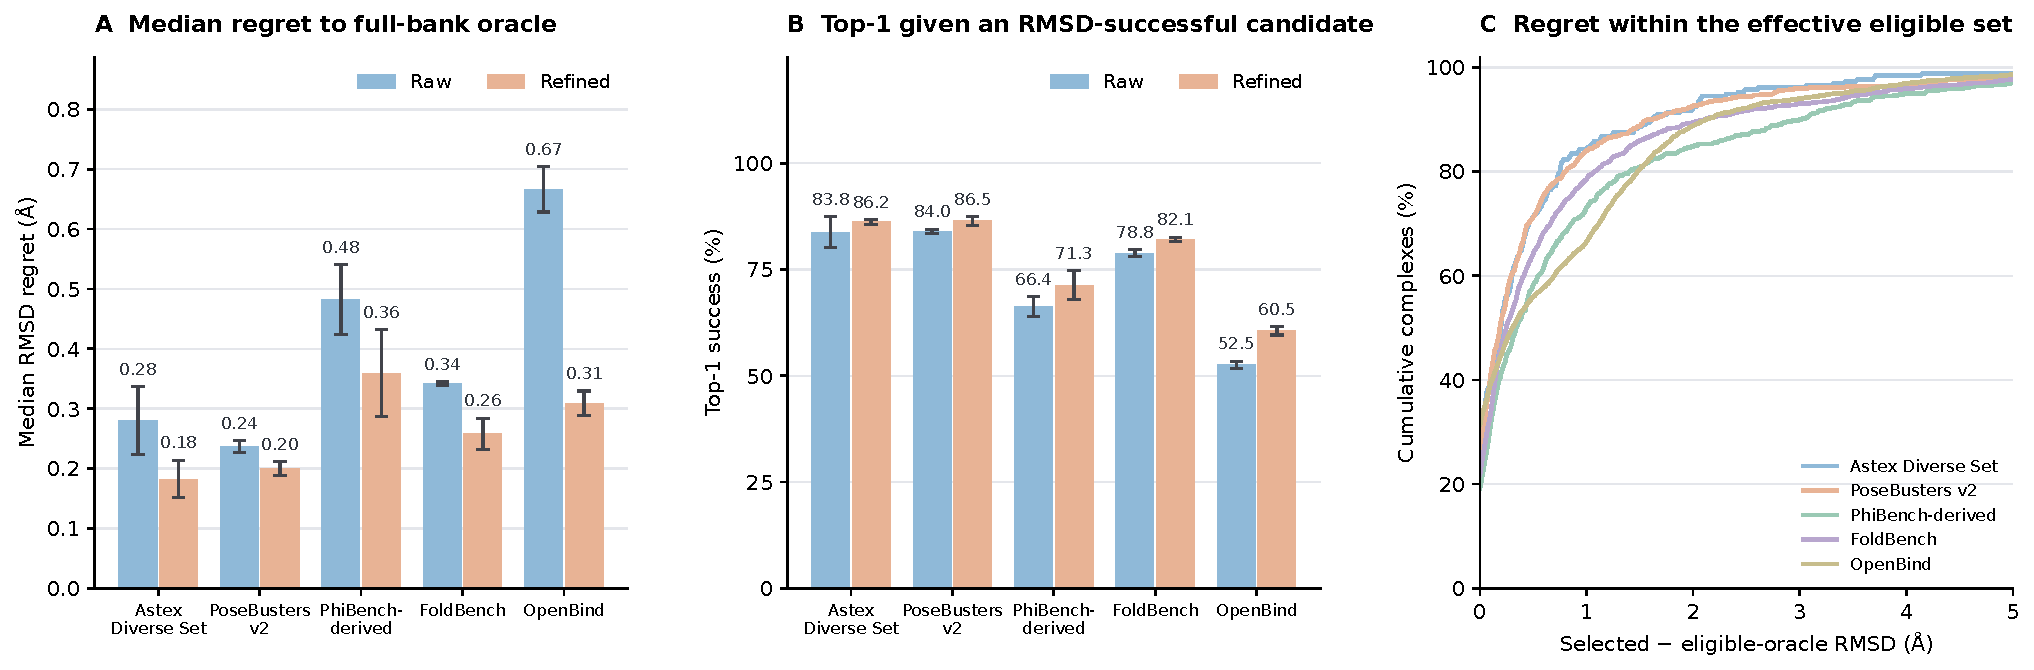
\includegraphics[width=\linewidth,keepaspectratio]{selection_regret.pdf}
    \caption{\textbf{Selection regret and conditional top-1 success.} \method results use the primary chirality-filtered confidence selector. (A) Median selected-minus-full-bank-oracle RMSD regret for raw and refined banks. (B) Selected top-1 RMSD success among complexes whose full bank contains an RMSD-successful candidate. Losses in A and B can include chirality-eligibility exclusions. (C) Cumulative refined selected-pose RMSD regret relative to the minimum RMSD within the same effective eligible set, including the unfiltered fallback when no candidate passes the mask. The corresponding outcome partition is shown in main Fig.~5C. Reference RMSD is used only for retrospective analysis. Bars show three-repeat means and sample SD.}
    \label{fig:selection-bottlenecks}
\end{figure}

\subsection{Generation-input sensitivity and guidance controls}

The sensitivity protocol in Online Methods crosses five crop radii with three center-jitter levels at prior scale \(2\,\angstrom\), and three prior scales with the same jitter levels at a \(10\,\angstrom\) crop. Three grid cells are shared. Four candidate-budget/guidance cells include the reused primary baseline, giving \(5\times3+3\times3-3+(4-1)=24\) unique conditions in total. The same three inference seeds are used for each complex. This analysis refines and rescores saved candidate banks from those prespecified generation conditions; it does not generate additional candidates. Raw and refined banks are scored with the actual source prior scale, which also enters the docking features recomputed for confidence. Neither refinement nor confidence scoring receives the perturbed center or generation crop. Refinement retains the original center and its \(18\,\angstrom\) receptor shell; confidence scoring retains the original center and its \(10\,\angstrom\) crop. These experiments therefore do not quantify end-to-end performance under a wrongly supplied pocket.

Paired conditions use the same seeds, fragment inventories and prior-draw construction. The jitter stream is independent of the pose prior; within each complex and repeat, jitter levels scale the same perturbation vector. Translation draws were identical; backend quaternion roundoff produced initial-rotation differences of at most \(2.81\times10^{-7}\) radians, without bitwise prior identity across backends. The 40- and 100-pose budgets are generated separately and are not nested banks.

Guidance controls add the capped energy drift in Eq.~\eqref{eq:si_guidance_drift}. Guided raw-bank mean RMSD--PoseBusters success was higher in both cohorts at each budget; refined-bank differences were smaller and had mixed signs (Fig.~\ref{fig:si-guidance-budget}). The primary protocol remains unguided.

\begin{figure}[!htbp]
    \centering
    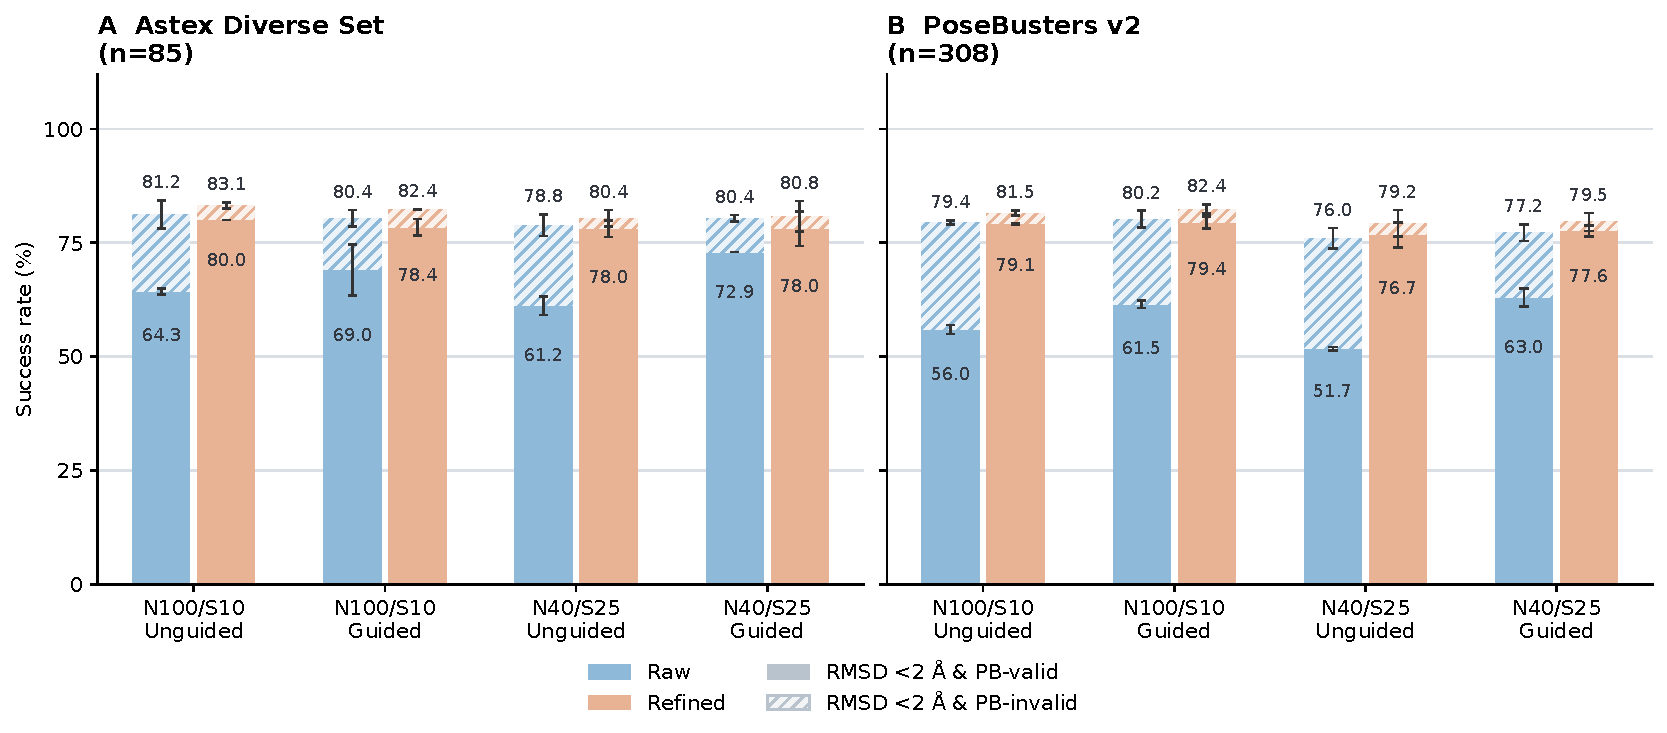
\includegraphics[width=\linewidth,height=0.64\textheight,keepaspectratio]{guidance_budget.pdf}
    \caption{\textbf{Guidance and candidate allocation at a fixed learned pose-step count.} (A) Astex Diverse Set (85 complexes) and (B) PoseBusters v2 (308 complexes). N denotes poses and S integration steps. Each 100-pose/ten-step (N100/S10) or 40-pose/25-step (N40/S25) condition uses 1,000 learned pose-steps, with unguided generation or normalized energy guidance of strength \(\eta=2\). Raw and refined banks use the input-chirality-filtered minimum-predicted-RMSD selector, with an unfiltered fallback. Solid segments show RMSD and PoseBusters success; hatched extensions show RMSD-successful but PB-invalid outcomes. Bars and whiskers show the mean and sample SD over three inference seeds. Guided and unguided initial draws are paired within each budget; the two budgets are separately executed. Equal pose-step counts are not equal-runtime comparisons.}
    \label{fig:si-guidance-budget}
\end{figure}


\begin{figure}[!htbp]
\centering
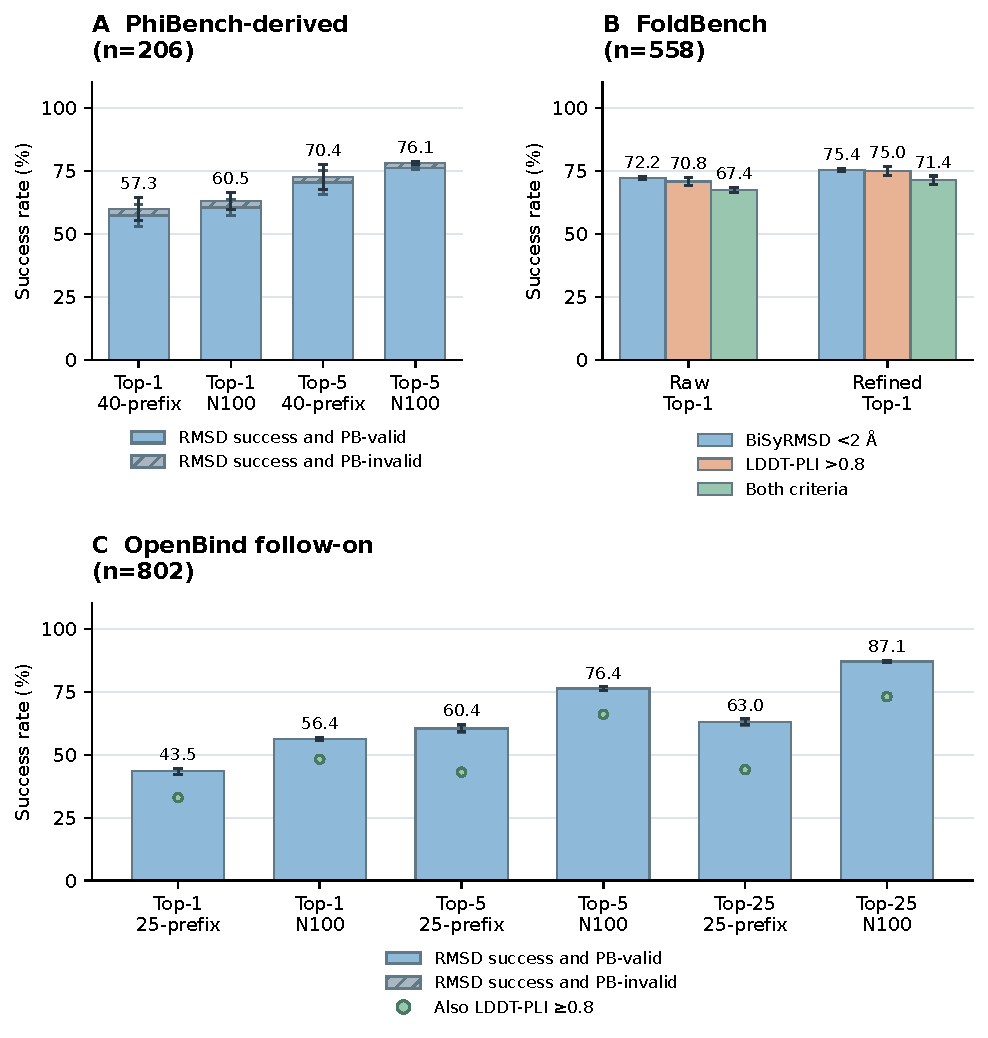
\includegraphics[width=\linewidth,height=0.70\textheight,keepaspectratio]{saved_endpoint_analysis.pdf}
\caption{\textbf{Benchmark-specific evaluation of saved candidates.} Supplementary endpoint analyses of saved EFF-Dock candidates; all panels show success rates in percent. (A) Top-1 and Top-5 fixed-receptor symmetry-corrected RMSD success (\(<2\,\angstrom\)), with and without all 27 non-RMSD PoseBusters checks, in the locally selected PhiBench-derived cohort. This is not asserted to reproduce the native PhysDock PAL-RMSD, cohort or 18-check conjunction. (B) Raw and refined Top-1 BiSyRMSD (\(<2\,\angstrom\)), LDDT-PLI (\(>0.8\)), and their same-pose conjunction on all 558 FoldBench interfaces using OpenStructure 2.8.0. The supplied holo receptor makes this a redocking evaluation rather than the source cofolding task. (C) Top-1/5/25 on the official 802 OpenBind follow-on IDs, using OpenStructure 2.11.1 BiSyRMSD \(\le2\,\angstrom\), PoseBusters 0.6.5, and the additional same-pose LDDT-PLI \(\ge0.8\) criterion. A and C use refined banks and the frozen chirality-filtered confidence selector, including its no-eligible-candidate fallback. Hatching denotes RMSD-successful but PB-invalid cases. 40-prefix and 25-prefix restrict the original saved N100 banks before selection; they do not represent fresh smaller-budget generation or equal compute. Numbers in A and C give RMSD--PoseBusters success; numbers in B give the corresponding criterion. Bars and error lines show means and sample standard deviations across three fixed-weight inference repeats. Rates retain the entire cohort denominator; endpoint-specific determinate denominators and unresolved counts are provided in the source data. Native preparation differences remain.}
\label{fig:si-native-endpoints}
\end{figure}

\clearpage
\subsection{Readout ablation}
\label{si:readout_ablation}

Fig.~\ref{fig:readout-ablation} reports the matched readout ablation described in Online Methods. Both arms were trained from scratch with identical data, configuration, seed, schedule and GPU type and evaluated at the terminal EMA checkpoint, as fixed before training. The direct arm reads fragment-node features with the same head structure and emits one polar translational and one axial angular vector per fragment, projected onto the observable subspace. Internal-validation rollout success was 11.1\% and 10.8\% (paired difference +0.3 percentage points; 95\% interval \(-0.8\) to +1.4). In unrefined Astex banks, oracle@100 was 89.4\% and 91.8\% (\(-2.4\); \(-5.9\) to 0.0) and oracle@10 51.8\% and 50.6\% (+1.2; \(-4.7\) to +7.1); in PoseBusters v2 banks, oracle@100 was 88.3\% and 87.0\% (+1.3; \(-1.0\) to +3.9) and oracle@10 53.2\% and 52.3\% (+1.0; \(-3.2\) to +5.2). Intervals are complex-level paired bootstrap intervals and do not include training-seed variation. Both reduced-budget models remain below the released model, whose raw-bank oracle@100 was 96.9\% on Astex and 94.6\% on PoseBusters v2, so these results compare readouts rather than estimating production performance.

\begin{figure}[!htbp]
    \centering
    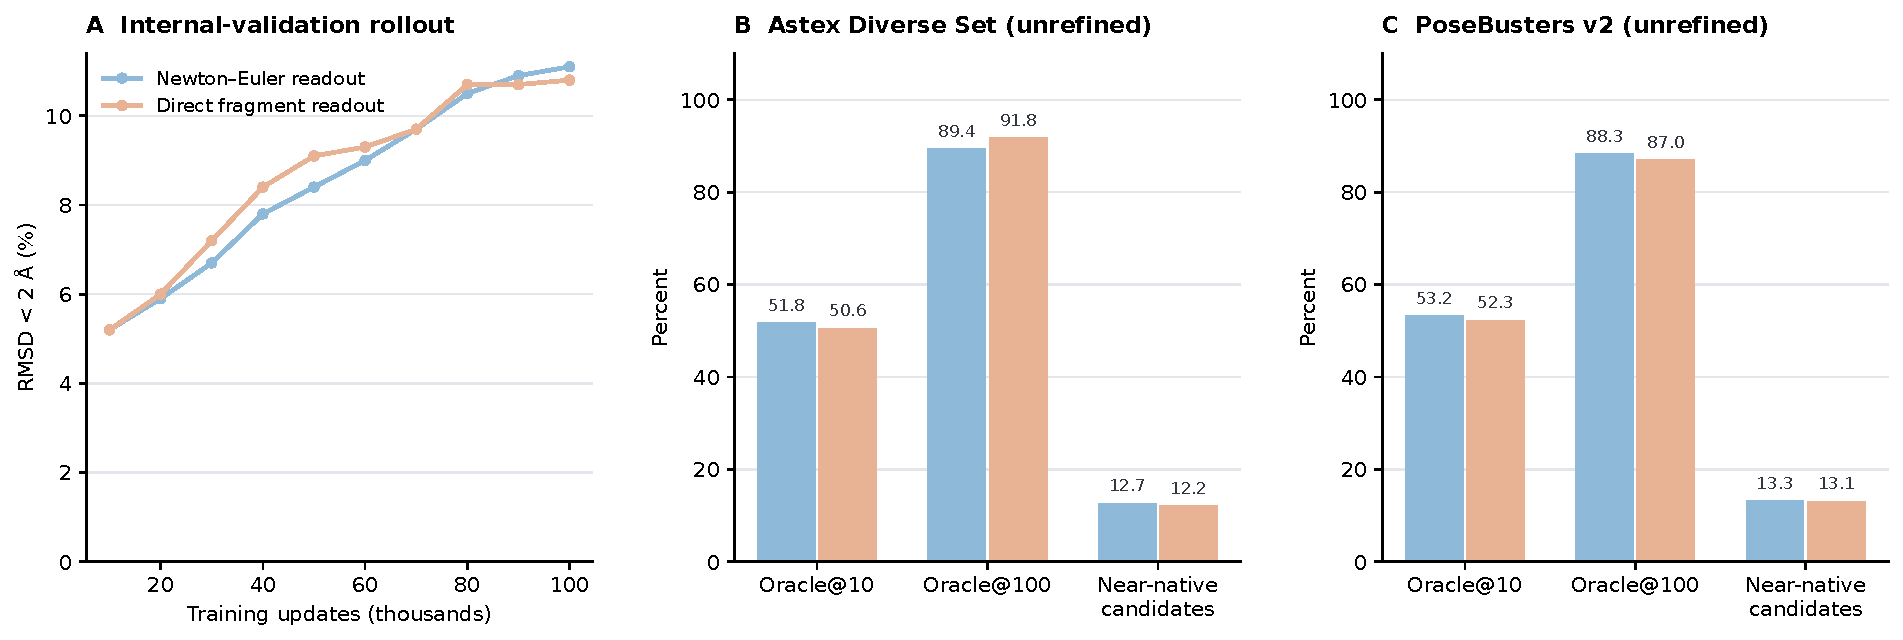
\includegraphics[width=\linewidth,keepaspectratio]{readout_ablation.pdf}
    \caption{\textbf{Matched readout ablation.} Two docking models trained from scratch for 100,000 updates with a global batch of 16 complexes differ only in the output head: the Newton--Euler least-squares readout of atom vectors or a direct fragment readout. (A) Internal-validation rollout success (single sample, 20 steps, 1,076 complexes) every 10,000 updates using the EMA weights. (B,C) Unrefined 100-pose, ten-step banks on Astex Diverse Set and PoseBusters v2 at the terminal checkpoint: RMSD \(<2\,\angstrom\) oracle coverage among the first 10 and all 100 generated candidates and the mean fraction of near-native candidates. One training seed per arm; no refinement or confidence ranking.}
    \label{fig:readout-ablation}
\end{figure}

\bibliographystyle{unsrt}
\bibliography{references}

\end{document}
